\documentclass[12pt,oneside]{book}
\usepackage[a4paper,width=150mm,top=25mm,bottom=25mm]{geometry}
\usepackage[utf8]{inputenc}
\usepackage{amsmath}
\usepackage{physics}
\usepackage{array}
\usepackage{graphicx}
\usepackage{emptypage}
\usepackage{listings}
\usepackage{xcolor}
\usepackage{rotating}
\usepackage{geometry}
\usepackage{ragged2e}
\usepackage{setspace}



%New colors defined below
\definecolor{codegreen}{rgb}{0,0.6,0}
\definecolor{codegray}{rgb}{0.5,0.5,0.5}
\definecolor{codepurple}{rgb}{0.78,0,0.82}
\definecolor{backcolour}{rgb}{0.94,0.95,0.95}

%Code listing style named "mystyle"
\lstdefinestyle{mystyle}{
xleftmargin=25pt,
  backgroundcolor=\color{white},
  commentstyle=\color{codegreen},
  keywordstyle=\color{blue},
  numberstyle=\tiny\color{codegray},
  stringstyle=\color{orange},
  basicstyle=\ttfamily\small,
  breakatwhitespace=false,         
  breaklines=true,                 
  captionpos=b,                    
  keepspaces=true,                 
  numbers=left,
  numbersep=5pt,                  
  showspaces=false,                
  showstringspaces=false,
  showtabs=false,                  
  tabsize=2
}

%"mystyle" code listing set
\lstset{style=mystyle}
\usepackage{caption}
\usepackage{subcaption}
\usepackage{hyperref}
\hypersetup{
colorlinks,
citecolor=black,
linkcolor=black,
urlcolor=black,
}

\graphicspath{ {Figures/} }


\begin{document}
\frontmatter
\begin{titlepage}
\begin{center}
\begin{singlespace}

\vspace*{0.7cm}
\Large
Universty of Tripoli\\
Faculty of Engineering\\
Department of Electrical and Electronic Engineering \\

\includegraphics[width=0.5\textwidth ]{Figures/UOT_Logo.png}            

\Huge
\textbf{Modeling, Control, and Experimental Validation of a Ball and Plate System}

\vspace{0.5cm}
\Large
A project submitted in partial fulfilment of the requirements for the
degree of Bachelor of Science in Electrical and Electronic Engineering

\vspace{1.2cm}
Prepared by:\\
\textbf{Mohammed S. Baayou}

\vspace{0.8cm}
Supervised by:\\
Dr. Ali S. ElMelhi
                   
\vspace{1cm}
\large
\textbf{Spring 2023}


\end{singlespace}            
\end{center}
\end{titlepage}
\newgeometry{left=5cm, right=5cm, top=5cm}
\chapter*{Dedication}
{\Large To my father, may Allah have mercy on him, and to my mother, may Allah protect her}

\chapter*{Acknowledgements}
\begin{center}
\begin{onehalfspacing}

\vspace*{0.7cm}
       
{\large 
First of all, thanks to Allah for giving me the ability, strength and aptitude to complete this project.
\vspace*{0.7cm}

I would like to extend my thanks and gratitude to my supervisor \textbf{Dr.Ali Elmelhi}, for his advises, suggestions, patience and encouragement throughout this project.
\vspace*{0.7cm}

I am deeply and forever obliged to thank my great family for their love, caring, support and encouragement throughout my entire life.
\vspace*{0.7cm}

Finally, I would like to thank to all the good friends that I have for their support and help, with special appreciation for \textbf{Mahmoud Karah} and \textbf{Salman Ajweeli}. \\
}
\end{onehalfspacing}
\end{center}

\begin{doublespacing}
\chapter*{Abstract}
{ \large This study presents an exploration of a real-time ball-on-plate system, encompassing the implementation, modeling, analysis, and control aspects. The primary objectives are to build a physical system, develop a dynamic model, design a PID controller, and compare simulation results with experimental outcomes. The initial phase involves the mechanical and electonical parts of the ball-on-plate system, discussing resistive touchscreen technology for ball position detection,filtering and sending.The modeling stage delves into the development of a dynamic model for the ball-on-plate system. The main parameters that affect the behavior of the system are determined using Euler's langrangian equation. The model is then simplified and linearized.The study analyzes the model, leading to the design and implementation of a PID controller. The manual tuning process is documented, and the resulting controller parameters are established. Challenges encountered during this phase, including unsimilarity between simulation and real-world responses, are discussed.
A comparative analysis between simulated and experimental outcomes provides valuable insights into the system's performance and the effectiveness of the designed PID controller.  }
\end{doublespacing}

\restoregeometry
\chapter*{Outline and objectives}
{\large 
\begin{onehalfspacing}
    
\section*{Outline}
The Outline of this Project is structured as follows: 
\begin{itemize}
    \item \textbf{Chapter 1} is an introduction contains abrief history of control theory the motivation to select our system, an literature review of previous works and overall project objectives.  
    \item \textbf{Chapter 2} describes the mechanical and electrical setup of the BPS selected and are used in this project.
    \item \textbf{Chapter 3} presents the mathematical modeling work, the linearization and simplifcation process, open loop validation and geometrical analysis to the linkage and servomotor in overall system.
    \item \textbf{Chapter 4} presents the design process of linear controllers including the theory of these controllers. 
    \item In \textbf{Chapter 5}, simulations and experimental results of each approach that have been raised in are presented then discussed. 
    \item Conclusions and Future Work of the project are presented in \textbf{Chapter 6}.
    \end{itemize}
\end{onehalfspacing}
\vspace{2cm}
\section*{Objectives}
The main objective of the project is to develop a dynamical model for 2-DOF Ball and plate system, study and develop a full mathematical model of the overall system, design PID controller, and finally implement and fabricate a lightweight BPS based on available parts in Libya and build it to test the PID controller actual performance}


\tableofcontents
\listoftables
\listoffigures
\mainmatter
\chapter{Introduction}
\graphicspath{ {Figures/chapter01} }
\section{Background and overview}
Control theory is a multidisciplinary field that plays a pivotal role in engineering and technology, providing a systematic framework for understanding, analyzing, and designing systems to achieve desired behaviors. At its core, control theory aims to regulate the output of a system, ensuring it conforms to a specified reference or trajectory. This field has far-reaching applications, ranging from industrial processes and aerospace systems to biological and economic systems.

The origins of control theory can be traced back to the early 19th century, with the advent of steam engines and the industrial revolution. Engineers faced challenges in maintaining the stability and efficiency of these complex mechanical systems. James Clerk Maxwell, a Scottish physicist, made early contributions with his Paper On governor—a mechanical device designed to regulate the speed of steam engines \cite{maxwell1868governors}. This marked the beginning of a systematic approach to controlling systems.

In the early 20th century, Norbert Wiener, a mathematician, and engineer, introduced the concept of cybernetics—a term derived from the Greek word for "steersman." Wiener's work focused on feedback systems and communication in both biological and mechanical systems. His seminal work, "Cybernetics: Or Control and Communication in the Animal and the Machine" (1948) \cite{wiener2019cybernetics}, provided a theoretical foundation for control theory.

Simultaneously, Aleksandr Lyapunov, a Russian mathematician, developed the theory of stability, which became a cornerstone in the analysis of dynamic systems. Lyapunov's stability theory laid the groundwork for understanding when a system would remain stable over time, a critical aspect of control system design \cite{lyapunov1992general}. 

The mid-20th century witnessed a surge in the formalization of control theory. Engineers and mathematicians began developing mathematical models and techniques to analyze and design control systems. Notable contributors during this period include Rudolf Kalman, who introduced the Kalman filter for state estimation \cite{kalman1960contributions}, and Richard Bellman, who pioneered dynamic programming as a method for solving optimization problems in control systems \cite{bellman1966dynamic}. The advent of computers in the 1950s and 1960s revolutionized control theory by enabling the implementation of complex algorithms for real-time control. This era also saw the rise of the field of optimal control.

In the latter half of the 20th century, control theory continued to evolve with the introduction of robust control techniques, adaptive control strategies, and the application of control theory to non-linear systems. The field expanded its reach into aerospace engineering, telecommunications, and other emerging technologies.

Today, control theory remains a dynamic and evolving field, with the ongoing researches into advanced control methodologies, researchers are in dire need of a real system on which to test advanced control methods and thesis.
The implementation of control systems in unstable physical systems is a critical aspect of engineering, as it addresses the need to stabilize systems that are prone to catastrophic failures. Textbooks on control systems often feature example problems involving such unstable systems, providing students with opportunities to study their behavior and explore various methods for designing and implementing control algorithms.

Two well-known examples of unstable systems used experimentally are the inverted pendulum and ball balancing systems on beams that shown in figure 1.1 or ball and plate. These systems serve as valuable educational tools, allowing students to understand the challenges associated with instability and the importance of control in maintaining stability. The study of these systems provides a foundation for exploring different control strategies and algorithms.

The ball and plate system (BPS) represents a extended and generalized version of the traditional ball and beam. In this system, a ball can freely roll on a rigid platform, and the inclination of the platform can be independently manipulated in two directions. 
\begin{figure}
    \centering
    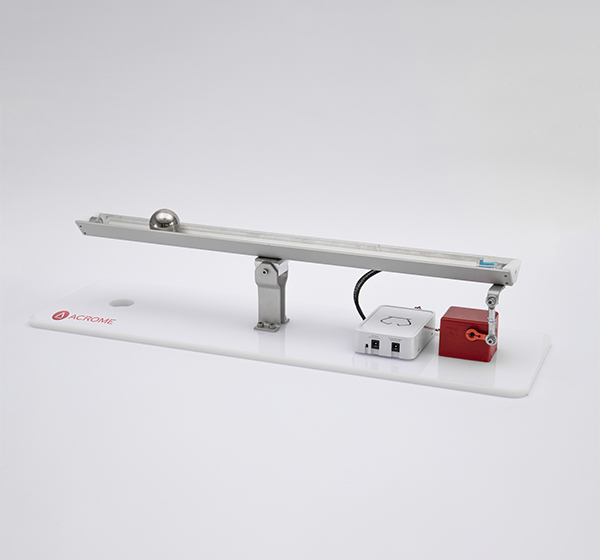
\includegraphics[width=0.7\linewidth]{ball-and-beam-new.jpg}
    \caption{Ball and Beam system}
    \label{fig:enter-label}
\end{figure}
The rigid plate, often equipped with a resistive touch panel or a camera, measures the position of the ball with respect to the center or a predetermined point on the plate. This system, by its nature, is inherently unstable, as even a minor disturbance can cause the ball to deviate significantly from its stationary position. Moreover, it lacks the ability to naturally return to equilibrium without external force intervention, which necessitating control methods for stability.

Everything we mentioned previously, in addition to the fact that the system is easily transportable, affordable, safe, has few malfunctions, scalable and controllable makes the BPS an ideal practical test environment for evaluating control methods in real-world scenarios. The main goal of the system is to keep the ball balanced on the plate within set boundaries or specific points. When the ball goes beyond these limits, a controller steps in, adjusting the plate's tilt in two directions to bring the ball back to its intended position.

To work effectively with the BPS, creating a precise nonlinear model is crucial for implementing model-based controllers. The Lagrange-Euler method is commonly used to derive the system's nonlinear equations by considering the kinetic and potential energies. Kinetic energy accounts for both linear and angular motions, while potential energies are calculated for all rigid bodies in the system. This method ensures a thorough understanding of the system's dynamics, facilitating the design and optimization of controllers tailored to its specific behavior.
 In our thesis we will work to design three different controllers to control the system theoretically and we will implement a PID controller to control the system experimentally then we will make a performance response comparison between these controllers.
 
\section{Literature review}
In general the previous works on ball-on-plate system can be classified based on several categories, Based on the type of the sensor used, based on actuation and linkage prototype or based on the controllers used to stabalize the system.

In \cite{awtar2002mechatronic}, \cite{ham2015development} Awtar and Ham introduced a prototype with a resistive touch screen and servo-motors for plate deflection. Another method in\cite{madhumitha2021design}, \cite{zhao2014multiple}, \cite{han2012tracking} and \cite{bdoor2016design} used a top-positioned camera for ball location extraction, while Debono \cite{debono2015application} employed a camera and computer algorithm for faster acquisition.
Dual pneumatic rotary cylinders in \cite{yuan2010modelling} provided a low-cost solution with good control accuracy, though with increased design complexity. Designs using metallic balls were common, but Das and Roy \cite{das2017improved} introduced a hollow plastic ball, automatically decoupling input parameters.

In the realm of control strategies for ball-on-plate systems, various approaches have been explored. Different controllers offer unique advantages and challenges in achieving system stability. Proportional-Integral-Derivative (PID) controllers, being a common choice, have been implemented in several studies \cite{adiprasetya2016implementation}, \cite{stander2017low}, \cite{betancourt2019fuzzy}, \cite{kassem2015commparison} and \cite{fabregas2017virtual}. Optimal control techniques have also been investigated. In \cite{jafari2012linear}, Hooshang Jafari. explored LQG control strategies, considering the kalman filter estimator in the system. Model Predictive Control (MPC) has been another area of interest, as showcased by Krzysztof Zarzycki and Maciej Ławryńczuk in \cite{zarzycki2021fast}, where MPC was employed for a comprehensive comparison with PID LQR controllers.




\chapter{System Setup and implementation}
\graphicspath{ {Figures/chapter02} }


This chapter describes the details of a mechanical BPS including a description of its mechanical parts, electrical and software that is used to control the system.

\section{Mechanical structure}
In order to balance a ball on a flat platform, there were several options and several designs that served this purpose, and each design had advantages and disadvantages that must be chosen between. Based on degree of freedom of the plate, Figure 2.1 demonstrate a different types of designs. to reduce the number of actuators and reduce the level of complexity in the platform, we chose the 2-DOF design since 2 is so enough to control the both axis of the plate.
To achieve this design six main parts was needed, the base, the joint, rods, servo holder, the plate and the ball.
\begin{figure}[h]
    \centering
    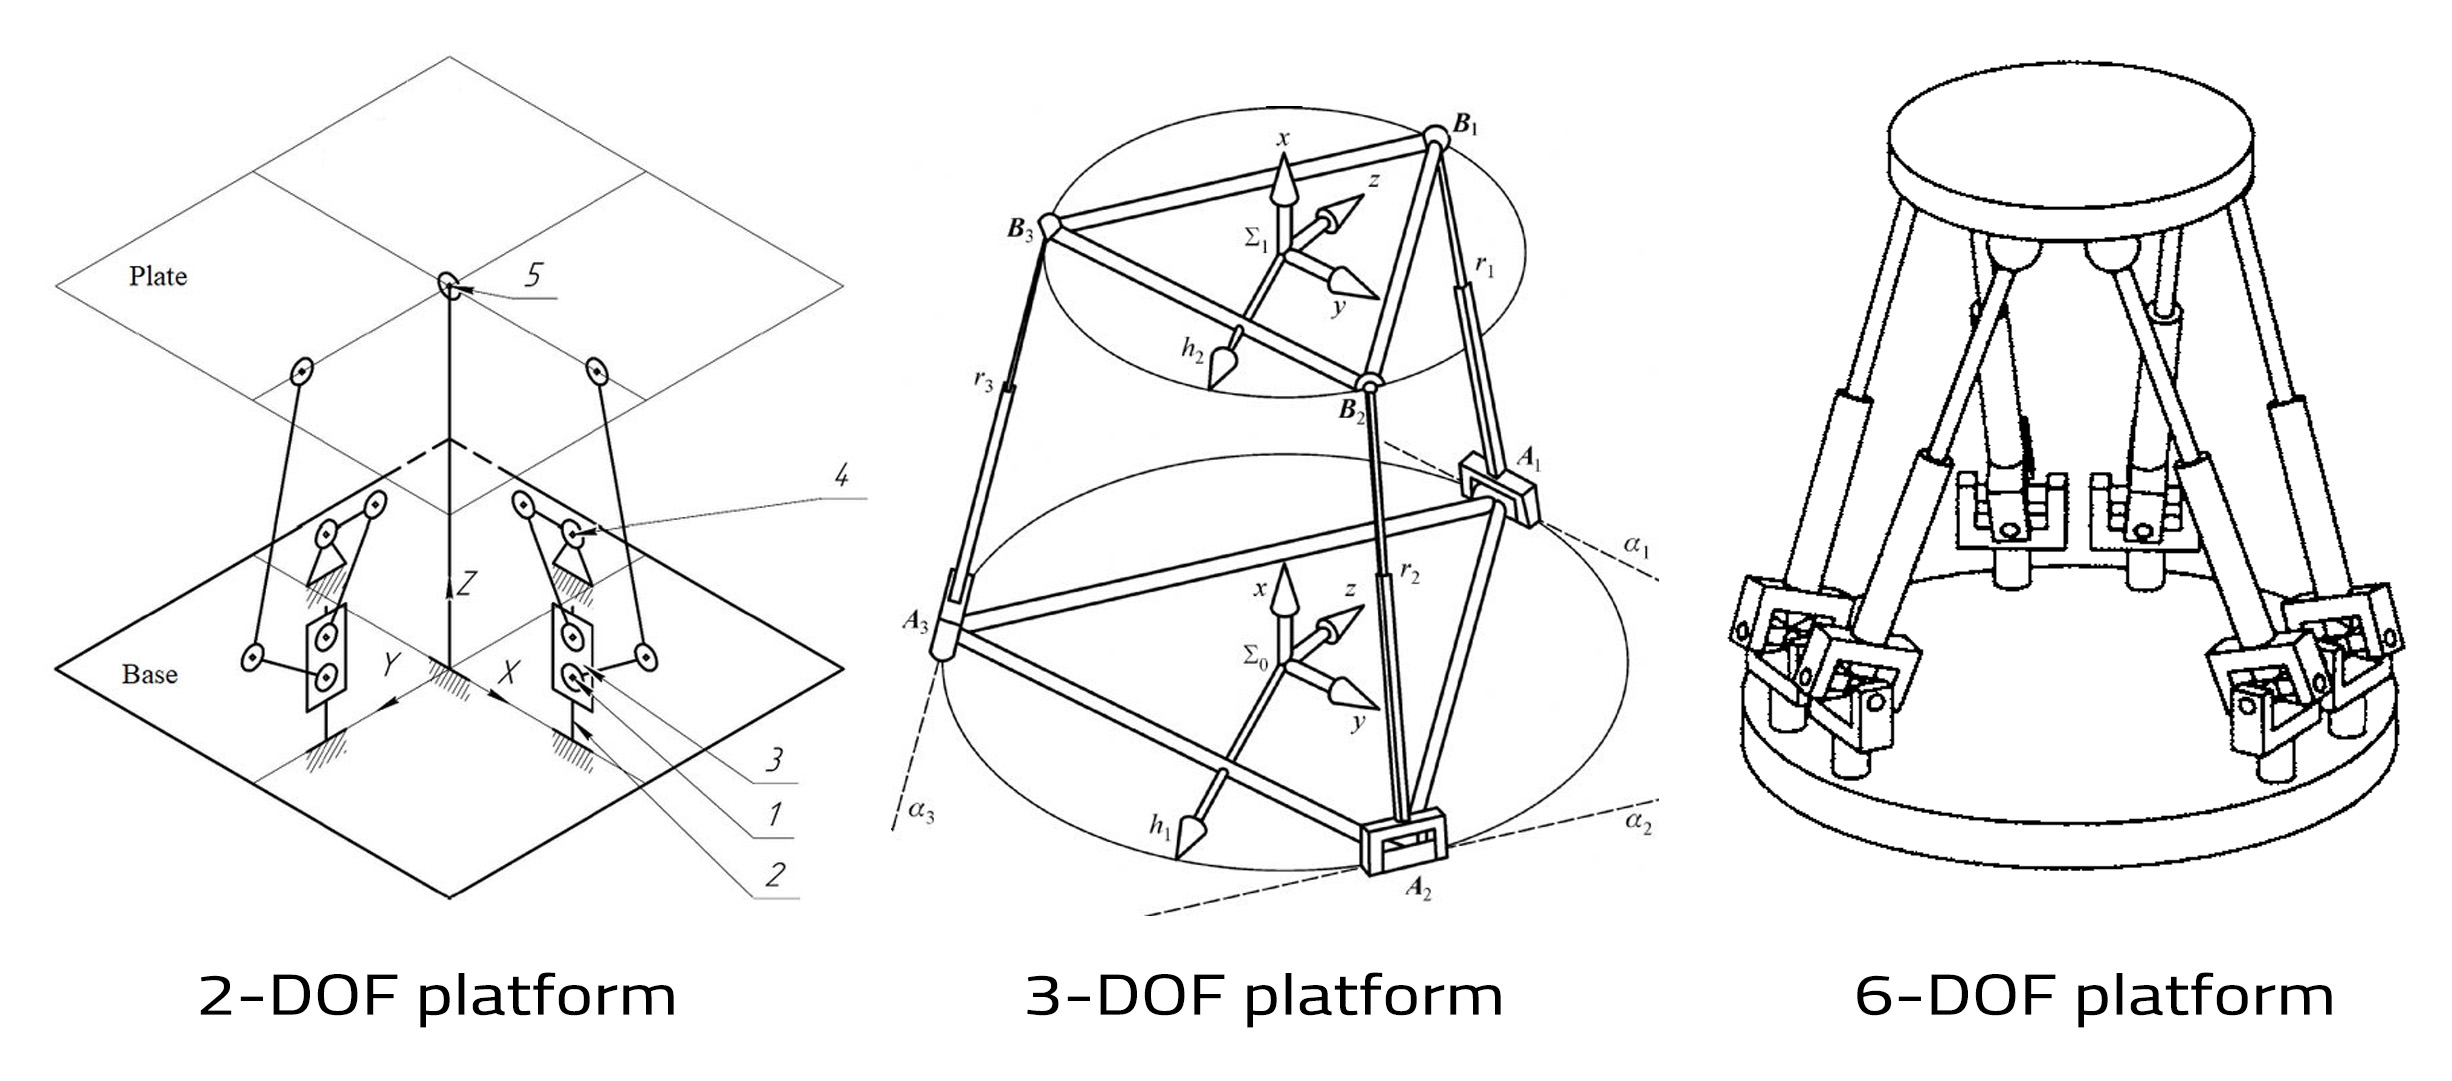
\includegraphics[width=1\linewidth]{DOF_Types_Platform.jpg}
    \caption{A variety of Ball and Plate System platform types based on the degree of freedom}
\end{figure}

\begin{itemize}
  \item \textbf{Base:} For the base a black rectangular piece of wood was selected with dimensions of 45 x 19.5 x 2 cm, this base serves as a main base on which the rest of the mechanical and electronic parts stand.
  
  \item \textbf{Joint:} the pivotal connection allowing the plate to move around two axes is crucial.Two types of joints were considered shown in figure 2.2: the universal joint and the ball joint. The ball joint was chosen for its superior flexibility, enabling smooth and responsive movements of the plate. This decision contributes to the overall adaptability and performance of the ball-on-plate system.
  
  \begin{figure}[h]
    \centering
    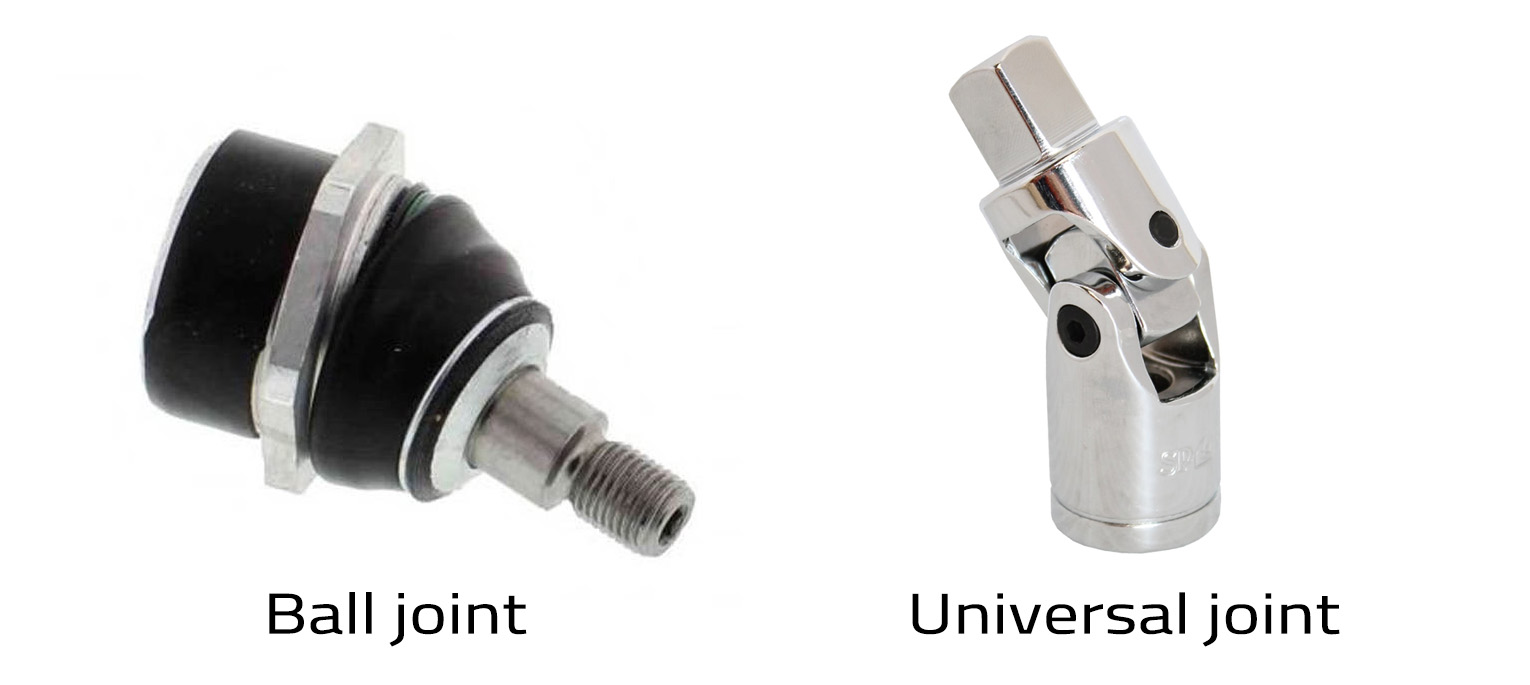
\includegraphics[width=0.9\linewidth]{joints.jpg}
    \caption{Two types of joints considered in the design - universal joint and ball joint}
    \label{fig:enter-label}
\end{figure}

  \item \textbf{Rods:} A linkage part between the servomotor and the plate that converts tho rotational movement into a linear motion, 20 degree at most of inclination is considered, so the angle relation with the dimension is analyzed and calculated in chapter 3
  
  \item \textbf{Servo Holder:} A simple aluminum structure that holds the servos in place, facilitating controlled movements and reduce the servomotor vibration, shown in figure 2.3.
  
\begin{figure}[h]
    \centering
    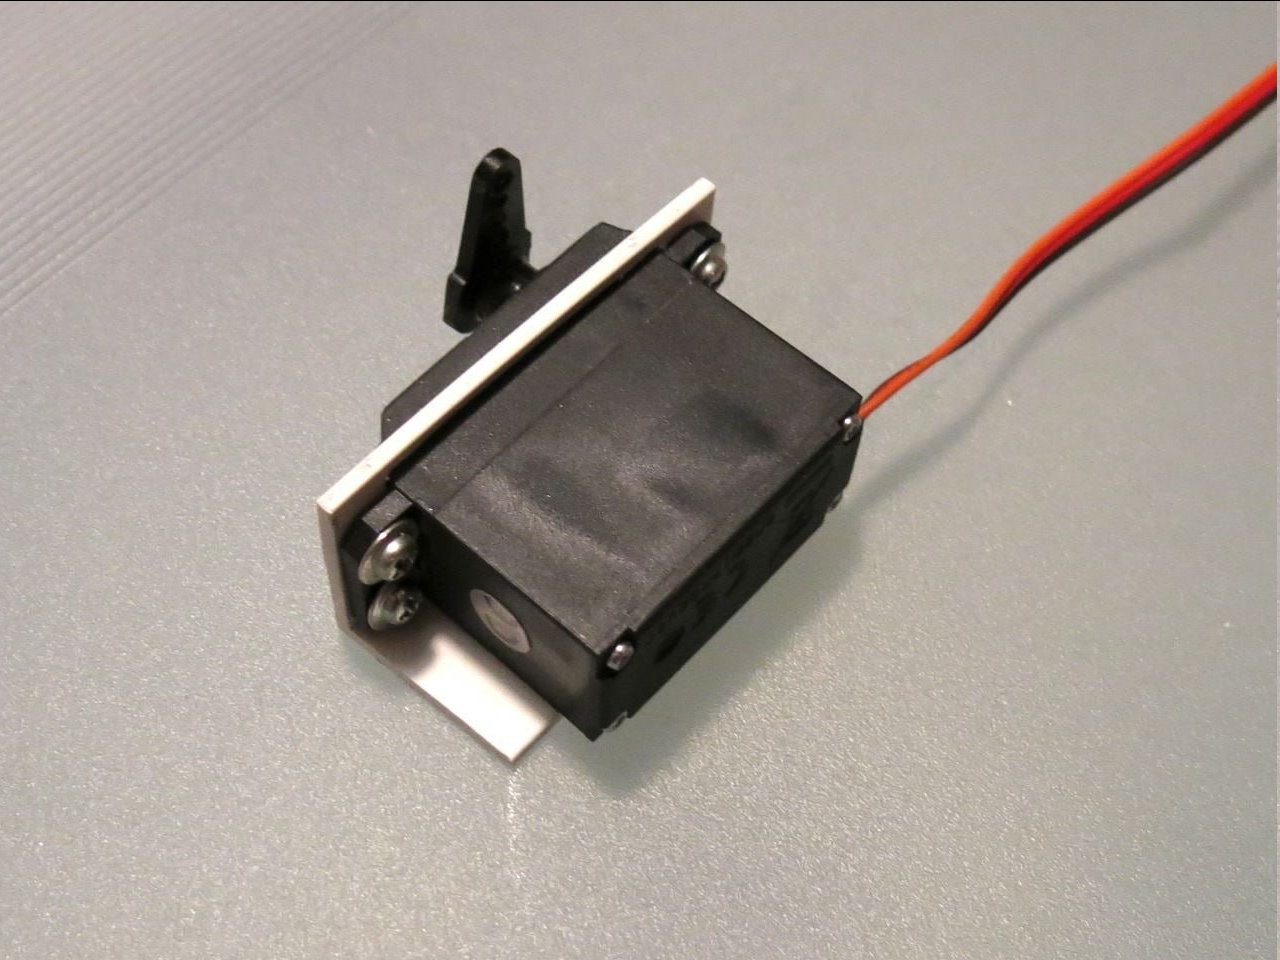
\includegraphics[width=0.55\linewidth]{Servomot_holder.png}
    \caption{The holder structure for the servomotor, ensuring controlled movements and reduced vibration}
    \label{fig:enter-label}
\end{figure}
  \item \textbf{Plate:} Transparent plastic flat platform where the ball rests.
  \item \textbf{Ball:} The object most be spherical symmetrical solid to be balanced on the plate , The ball’s mass should be not lower than 70 g. If the force is too small, two different effects can be observed: no touch is detected and the sensor returns Not a Number (NaN) signal or the ball is temporarily detected in a different place
\end{itemize}

\section{Electrical parts}
The circuit used and all the electrical parts are shown in figure 2.4
\begin{figure}[h]
    \centering
    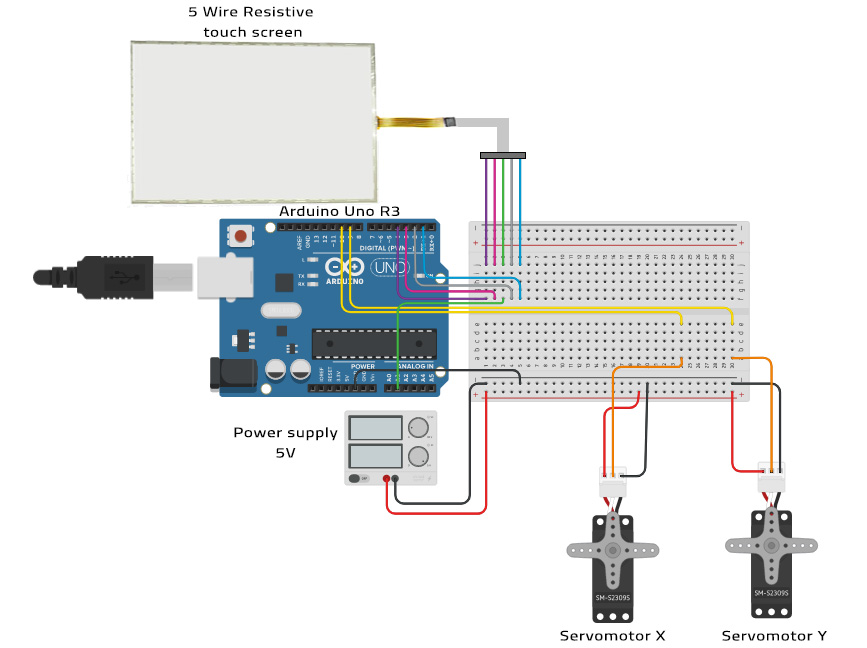
\includegraphics[width=1\linewidth]{Arduino_schematic.jpg}
    \caption{ Basic schematic illustrating the electrical components and circuitry of the System}
    \label{fig:enter-label}
\end{figure}
\subsection{Actuators}
For our 2-DOF plant, where the plate tilts around its center, two actuators are required to control tilt along the X and Y axes. Accuracy is crucial for achieving zero steady-state error. The Servo motor and stepper motor shown in figure 2.5 are the most suitable choices.\\
\begin{figure}[h]
    \centering
    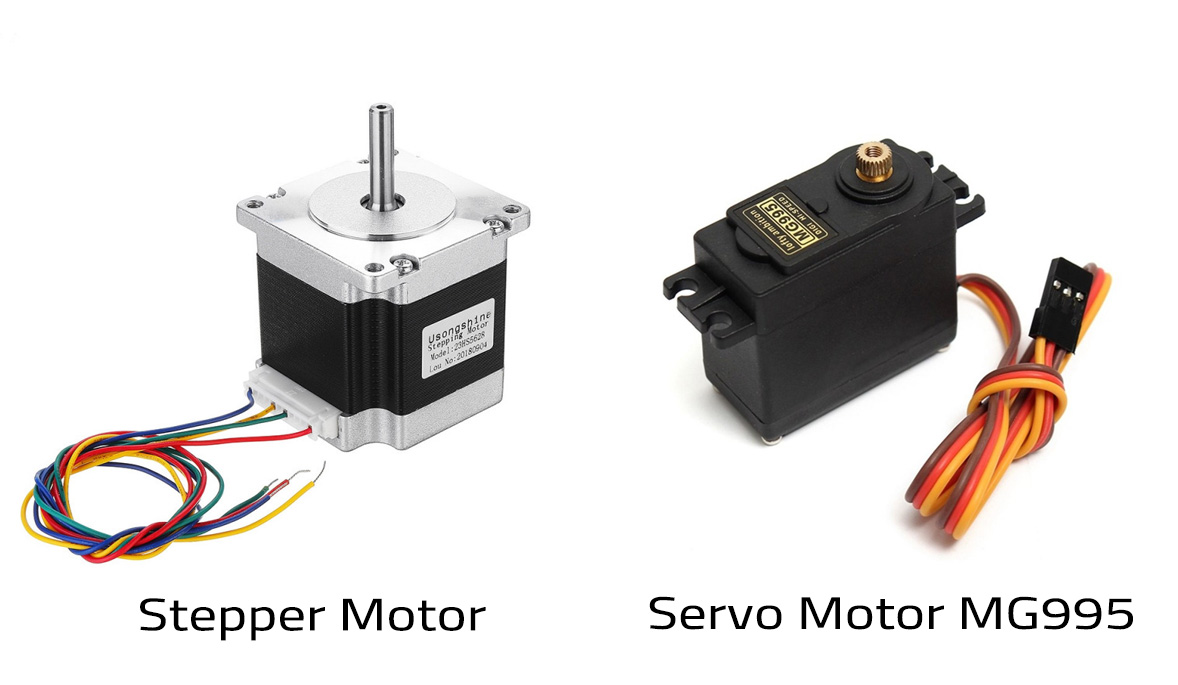
\includegraphics[width=0.75\linewidth]{Actuators_types.jpg}
    \caption{Types of actuators explored for the 2-DOF system - Stepper Motor and Servo Motor}
    \label{fig:enter-label}
\end{figure}

\textbf{Stepper Motor:}
\begin{itemize}
    \item Comes without an encoder or drive, requiring separate purchase, installation, and control.
    \item Relatively more expansive 
    \item Encoder feedback is used to eliminate missed steps.
    \item Torque decreases with speed, and steppers consume continuous current unless controlled not to.
\end{itemize}

\textbf{Servo Motor:}
\begin{itemize}
    \item DC motor with a gearbox for speed reduction and higher torque.
    \item Internal circuitry includes an encoder/potentiometer and controller.
    \item Powered by two cables and commanded via Pulse-width modulation(PWM).
    \item Consumes current only when needed, running cooler.
\end{itemize}

Servomotors are used as the actuators. The choice has been motivated by the fact that servos do not require the use of an additional control loop for engine rotation. Additionally, their relatively low cost is also an essential advantage. The servomotors are equipped with a proportional controller. The Pulse Width Modulation (PWM) signal is used to control them, the pulse cycle is equal to 20 ms and pulse width is in the 1000–2000 \(\mu\)s range. Their rotational range is \(60\deg\), the maximum speed is 0.5 s/\(60\deg\).
\subsection{Sensor}
In the BPS, achieving accurate ball location detection is fundamental for effective control. For this purpose, we explored various sensor options. While alternatives like cameras, infrared sensors, and capacitive systems are available, we went for resistive touch screens due to their versatility and cost-effectiveness. In particular, we have chosen the 17'' 5-wire resistive touch screen pad (Width of the panel was 355 mm, its height was 290 mm)

A five-wire resistive touchscreen, much like its four-wire counterpart, comprises two transparent resistive plates separated by insulating spacers. In this configuration, the top plate features a metalized contact, serving as the voltage sensing node. The bottom plate's four corners generate voltage gradients in both the x and y directions (refer to Figure 2.6).
\begin{figure}[h]
    \centering
    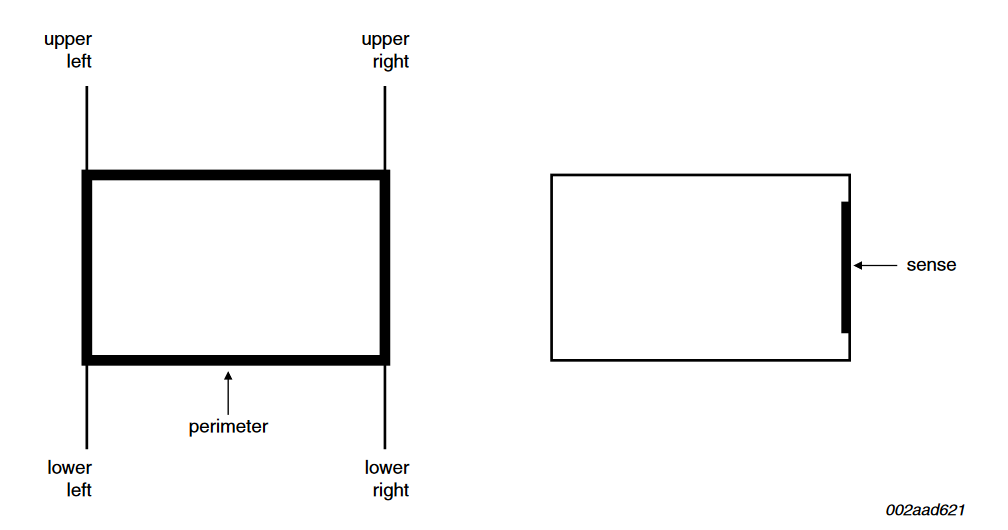
\includegraphics[width=1\linewidth]{structure_5_wire.png}
    \caption{Structure of 5-wire resistive touch screen}
    \label{fig:enter-label}
\end{figure}
The way the touchscreen works is by setting up specific ways for measuring both sideways (x-direction) and up-down (y-direction). When you press the screen with enough force, the top part bends and touches the bottom part. Figuring out the resistance in a 5-wire touchscreen can be a bit complex, but the addition of circuits along the edges of the touchscreen makes it simpler to think of it like a tool that divides voltage at the spot where it's touched. This, of course, depends on using the right setup called biasing.

Biasing the upper left and right corners to Vss and biasing the lower corners to Vdd enables measurement of the y-coordinate. Conversely, biasing the left side to Vss and the right side to Vdd facilitates measurement of the x-coordinate. Simultaneously biasing all four corners to Vss serves to detect when the screen is touched, triggering an interrupt (see Figure 2.7).
\begin{figure}[h]
    \centering
    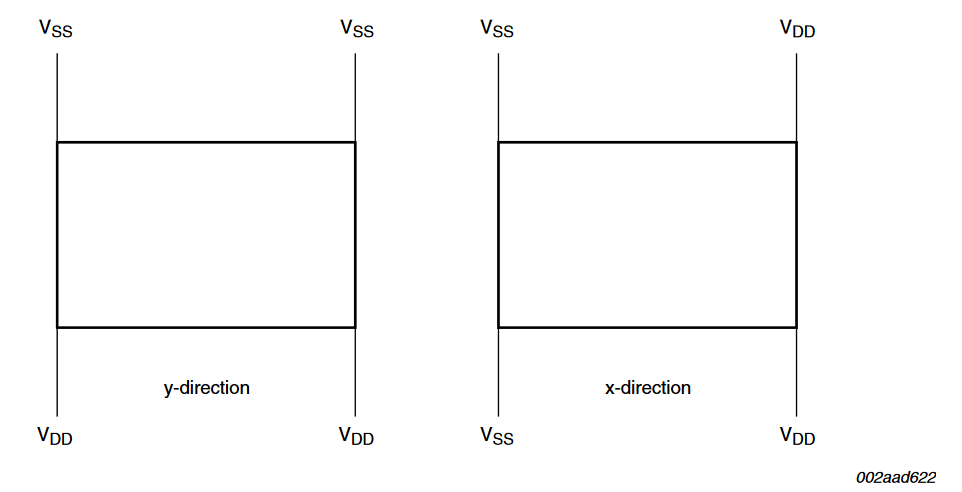
\includegraphics[width=1\linewidth]{Touchscreen_reaading.png}
    \caption{ Biasing setup for reading x and y directions of a 5-wire resistive touch screen}
    \label{fig:enter-label}
\end{figure}
In the touch condition, the sense signal from the screen connects to a port pin programmed as an input with a high resistance pullup. All corners of the touchscreen are driven to a logic zero. When touched, a voltage divider is established between the internal pullup of the port pin and the resistance of the touch screen. Notably, the resistance of the touch screen is significantly lower than the pullup connected to the sense signal. Consequently, when a touch occurs, the voltage at the sense signal pin approaches zero, initiating an interrupt.the biasing and measurement requirements for each of the four wires of the touchscreen are summarized in Table 2.1 .
\begin{table}[h]
\centering
\caption{Touchscreen interface requirements}
\label{tab:touchscreen_requirements}
\begin{tabular}{|p{2.5cm}|c|c|c|c|p{2cm}|}
\hline
\textbf{Function} & \textbf{Upper left} & \textbf{Lower left} & \textbf{Upper right} & \textbf{Lower right} & \textbf{Sense} \\ \hline
Hardware touch detection & Vss & Vss & Vss & Vss & Logic zero interrupt \\ \hline
Read x-position & Vss & Vss & V\tiny{DD} & V\tiny{DD} & Voltage measurement \\ \hline
Read y-position & Vss & V\tiny{DD} & Vss & V\tiny{DD} & Voltage measurement \\ \hline
\end{tabular}
\end{table}

The touch panel, while effective, has some disadvantages. It's highly sensitive to disturbances, requiring sufficient pressure into the plate, If the force of the touch is too small, two issues can arise: either no touch is detected, resulting in a NaN signal, or the touch is temporarily detected in a different location than its actual position. While these problems are rare when the ball is stationary, constant rolling can introduce measurement errors. Additionally, tilting the plate can reduce the gravity force component perpendicular to the plate, making the pressure force on the screen insufficient.

To mitigate these issues, several filters are employed:
\begin{enumerate}
    \item A filter detects when the sensor stops detecting the ball, and the touch panel returns invalid position values (zero, NaN or etc). When identified, the filter ignores these values, using the last meaningful number as the current position.
    \item lowpass filter that identifies high magnitude spikes when the sensor detects an incorrect ball position. If the current position change exceeds a certain threshold, it is ignored.
    \item An arithmetic filter collects n measurements of the ball position and calculates it as the sum of the measurements divided by n.(An average and median filters was considered to select in between).
\end{enumerate}

\subsection{Microcontroller}
In this work, two approaches to control the system was implemented, in the first approach Arduino Uno R3 was used as a microcontroller,Through it, the sensor data is retrieved and filtered, then through the same Arduino the PID signal is calculated and given to the servomotor as an output. in the second approach, the Arduino only played the role of data acquisition from the sensor to send it to the PC through a serial communication. The computer, using Simulink, processes the data, filters it, controls it, and sends the control signal to the Arduino again, which in turn sends it to the servo motor.
\begin{figure}[h]
    \centering
    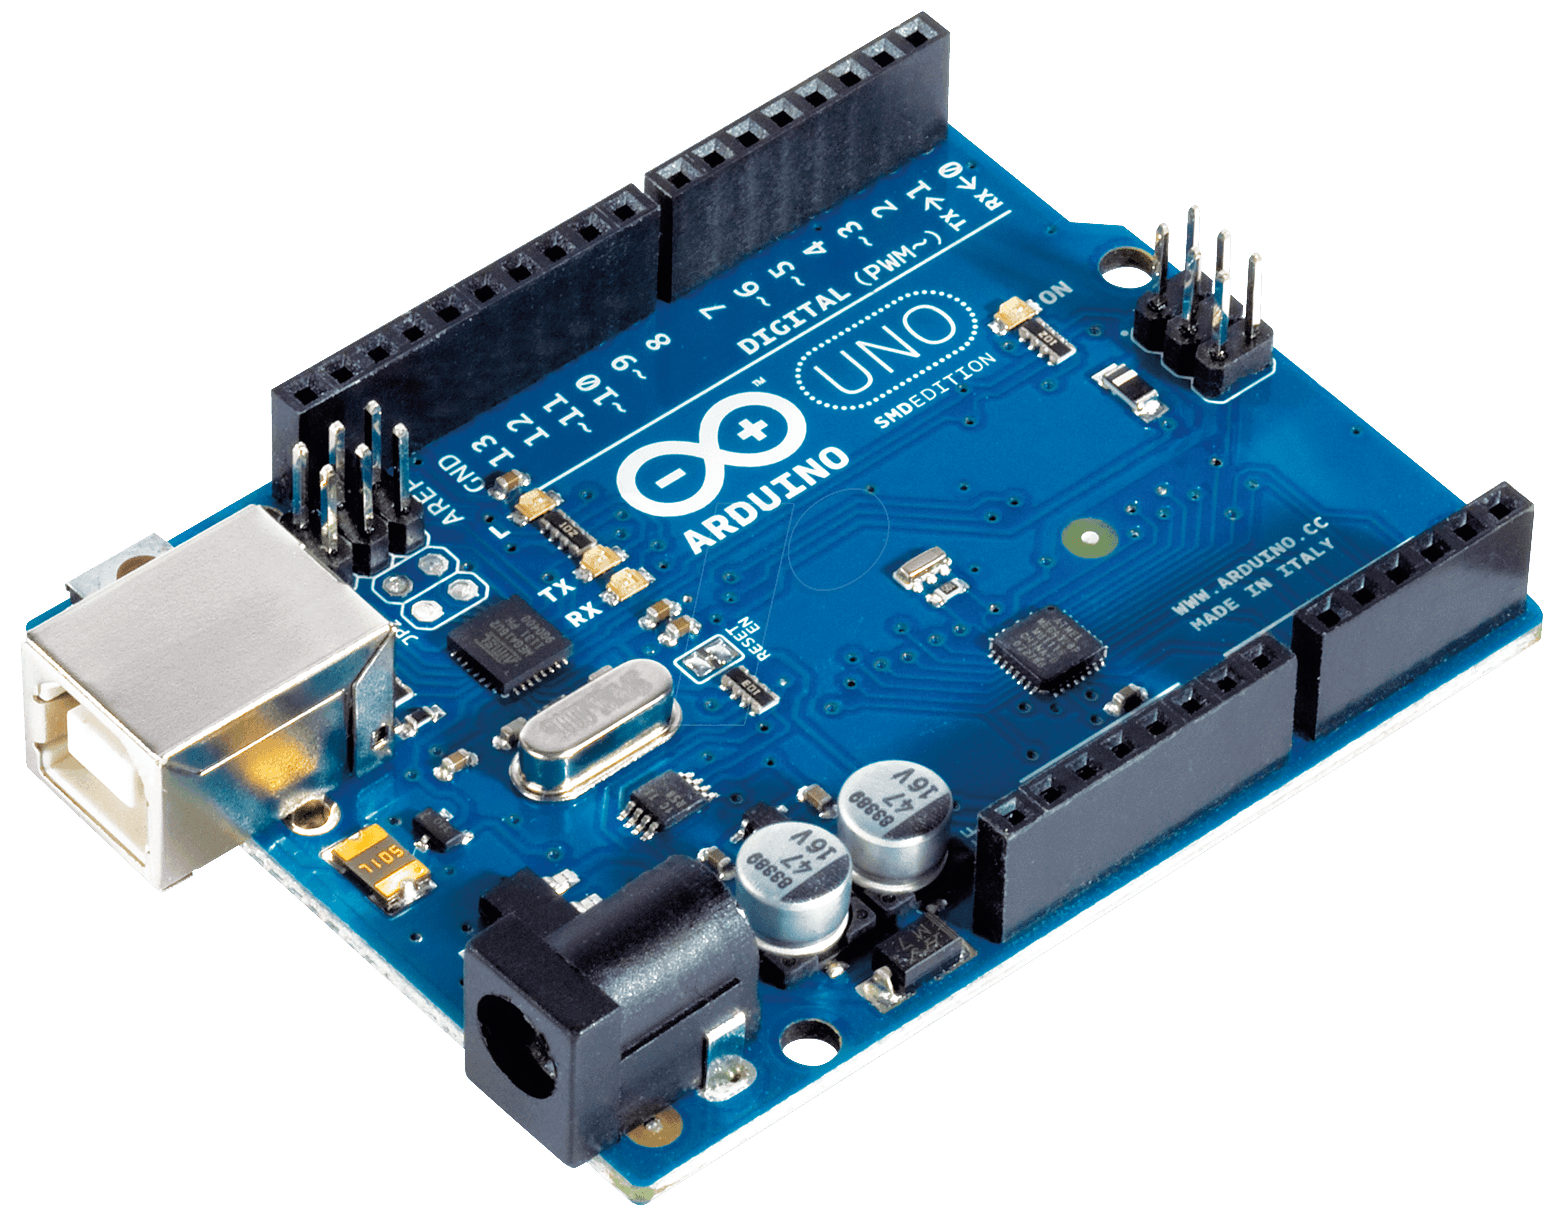
\includegraphics[width=0.75\linewidth]{ArduinoUnoR3.png}
    \caption{microcontroller: Arduino Uno R3}
    \label{fig:enter-label}
\end{figure}
Arduino Uno is a microcontroller board based on 8-bit the ATmega 328P. It has 14 digital input/output terminals, where six of them can be used as a pulse width modulation (PWM) outputs. It has six analog inputs, a 16 MHz quartz crystal,a USB connection, a power jack, and a reset button

\section{Software}
This section provides a concise overview of the software design methodology. For the full code implementation, please refer to the appendix A
The Arduino software consists of three primary components. The first component handles the acquisition of coordinate positions from the sensor. The second component deals with serial communication, enabling the exchange of data between the Arduino and the PC. Finally, the third component is devoted to the control section, managing the operational control of the system.


\subsection{Acquisition of coordinate positions}
The implementation of the algorithm for acquiring coordinate positions involves utilizing a 5-wire resistive touch screen, as illustrated in the figure 2.9.
\begin{figure}[h]
    \centering
    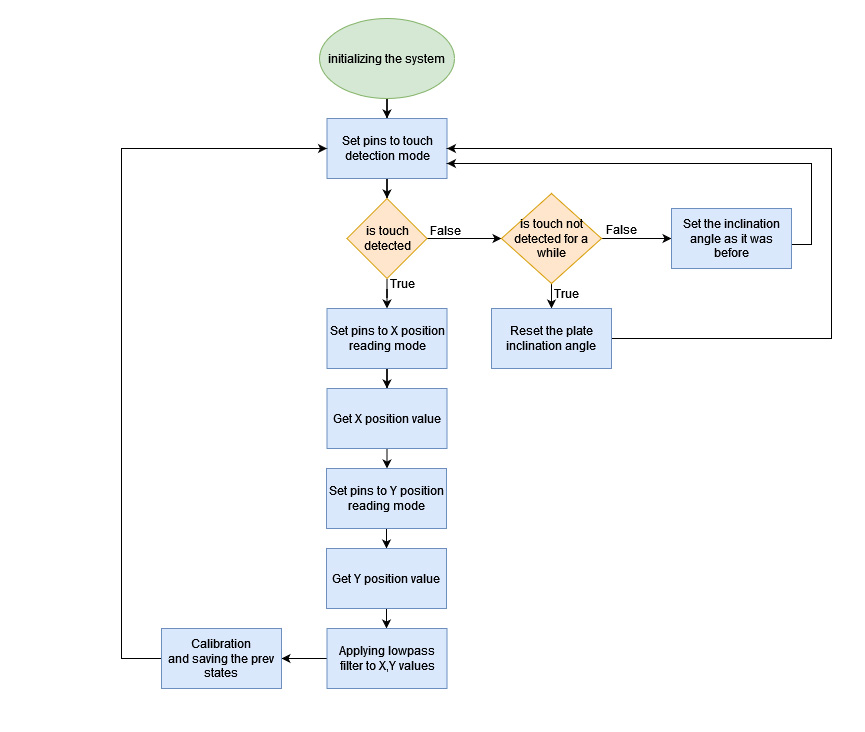
\includegraphics[width=1\linewidth]{touch_screen_algorithm_flowchart.jpg}
    \caption{Flowchart outlining the algorithm for acquiring coordinate positions from the resistive touch screen}
    \label{fig:enter-label}
\end{figure}
The flowchart illustrates the data retrieval process from the sensor, which progresses through several stages. Initially, we set the sensor to a "Stand By Mode". Upon detecting a touch on the screen, if the touch happens we instruct the sensor to capture the signal along both the X-axis and Y-axis. Subsequently, we filter the obtained readings via a lowpass filter. The figure 2.10 below demonstrates the signal's shape before and after passing through the Low-pass filter. Following the filtering, we convert the coordinates of the readings into centimeters.

\begin{figure}[h!]
    \centering
    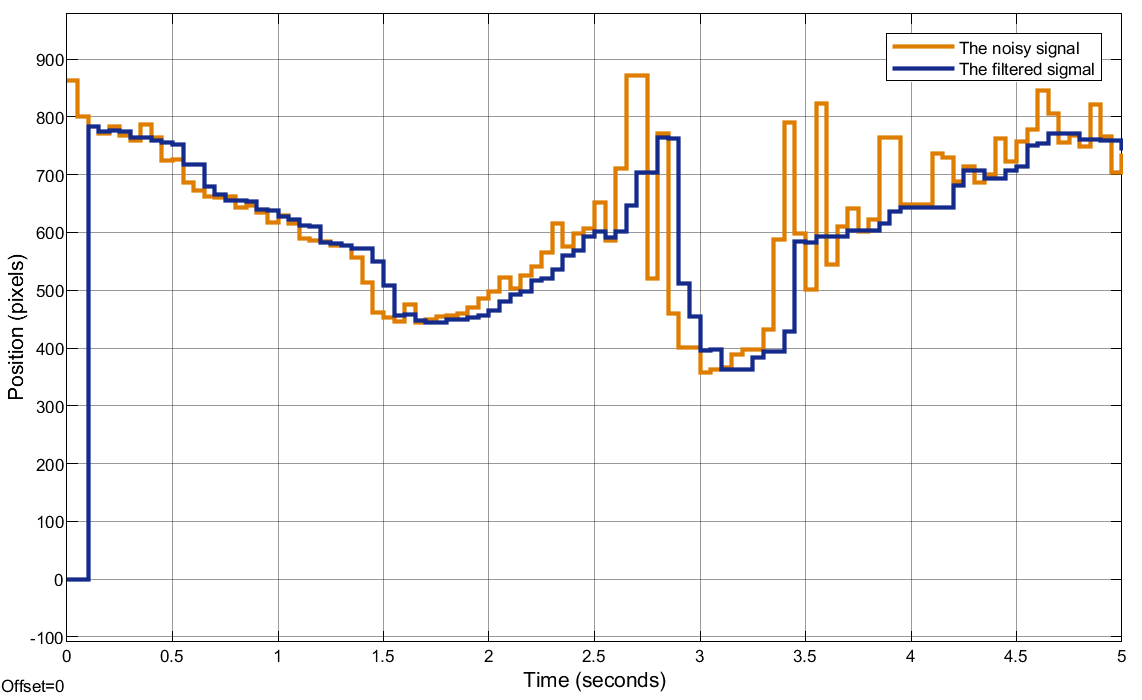
\includegraphics[width=1\linewidth]{Filter_vs_noisy_signals.png}
    \caption{Signal comparison before and after applying a low-pass filter to the resistive touch screen readings}
    \label{fig:enter-label}
\end{figure}

\subsection{Data transmission via serial communication}
Once we figure out where the ball is on plate through the Arduino, we want to share that information with the PC (Simulink). We use something called the "serial communication protocol" to send this data from the Arduino to the computer through a USB connection. Additionally, we want the computer to send back calculated output about the servomotor angle to the Arduino.

Using Instrument Control Toolbox in Simulink we could send and receive bytes in Arduino and interpret it as floats numbers, in the figure 2.11 we used Serial Configuration, Serial Send, Serial Receive blocks, cast to double block and byte pack which converts single data type to 4 packing bytes using byte alignment 4 with a header and terminator 
\begin{figure}[h!]
    \centering
    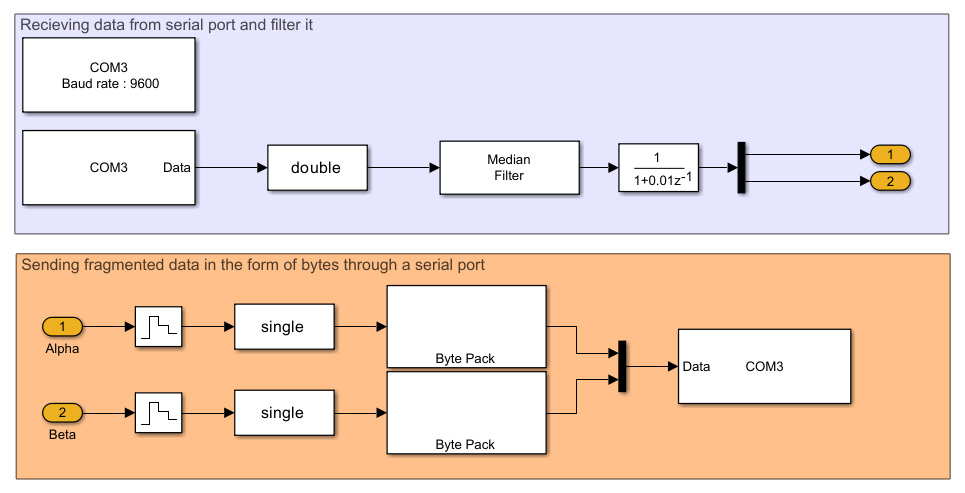
\includegraphics[width=1\textwidth]{Recieving_sending_via_serial_port.jpg}
    \caption{Serial communication setup using Simulink for data transmission between Arduino and PC}
\end{figure}

On the Arduino side, we used a union type to convert a float into an array of bytes (uint8). To receive the bytes from matlab, a function named getFloat()  was defined that converts each four bytes into float, as outlined in the code snippet presented in Figure 2.12.

\begin{figure}[h!]
    \centering
    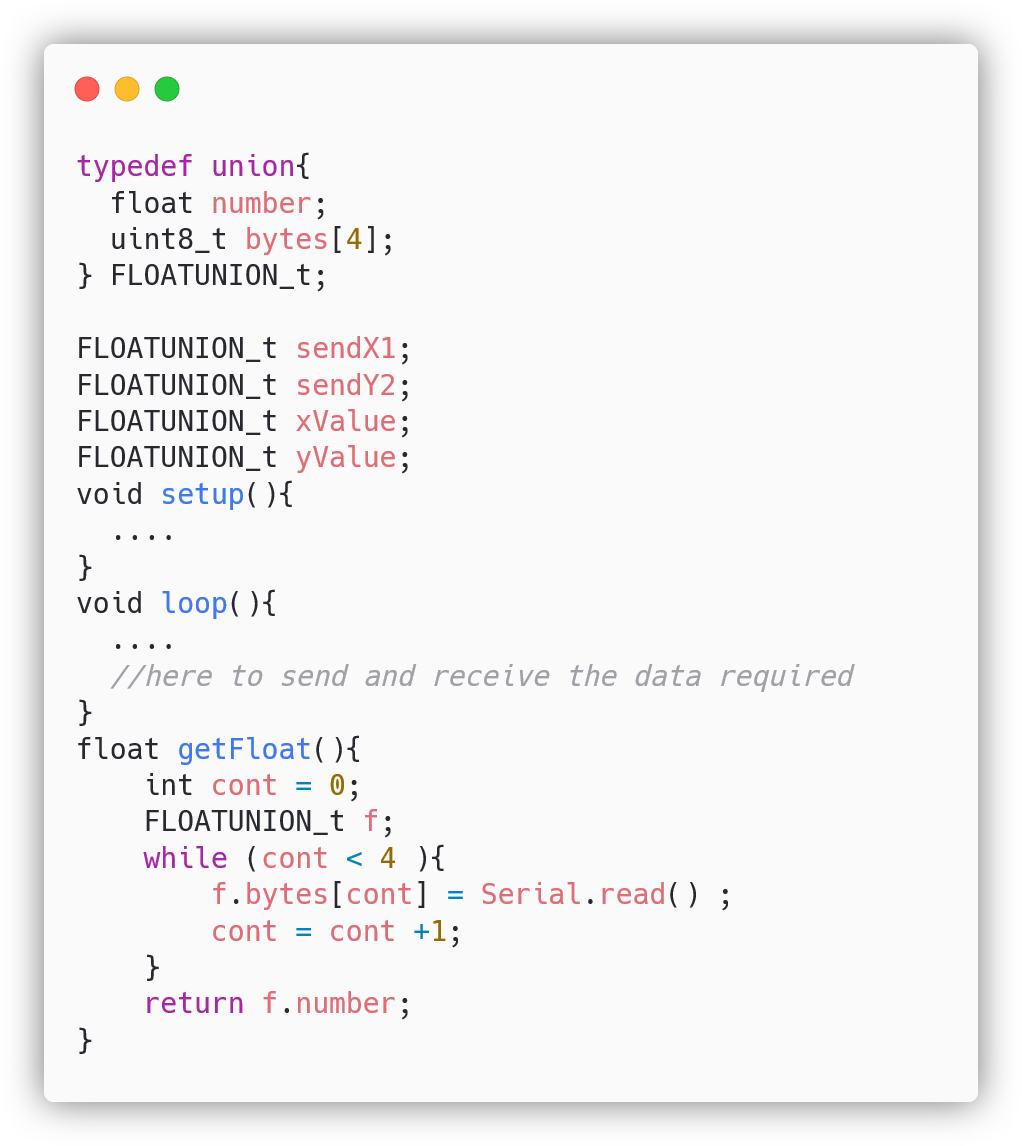
\includegraphics[width=0.8\textwidth]{carbon.png}
    \caption{Code snippet showcasing Arduino-side implementation for receiving and sending data via the serial port}
\end{figure}

\subsection{the operational control of the system}
To calculate the appropriate servomotor angle we used two methods one By by using serial communication and simulink control toolbox to control the system and the other by using the Arduino PID library designed by Brett Beauregard, in the first algorithm, the code running on the workstation communicates with the Arduino by a serial COM, therefore, the speed at which the Arduino respond is defined by the baud-rate, however the latter method is to be working in lower sampling time because there is no delay that occurs during data transfer


\chapter{Mathematical Modeling and Linearization}
\graphicspath{ {Figures/chapter03} }
\section{System Schematics}
The Ball and Plate (BPS) system is unstable, nonlinear, multi-variable, and under-actuated, The BPS model is an extension of the classical Ball and Beam system. It consists of a rectangular flat plate fixed movable at its center by a universal joint. The control target is the plate which could rotate about 2 mutually perpendicular axes
\begin{figure}[h]
\centering
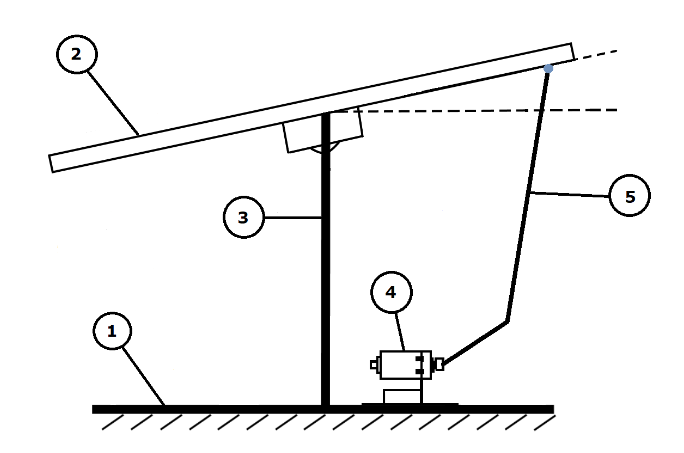
\includegraphics[width=0.5\textwidth]{BPS2DView}
\caption{Side projection of a BPS}
\end{figure}
The mechanical parts of the BPS are illustrated in Fig. 2.1, which contains;
\begin{enumerate}
\item The BPS wooden base carries all the other components of the system.
\item Plate is a plastic holder and a resistive touch screen sensor.
\item The central shaft is used between the structure base and the middle of the plate holder. Its job is to hold the plate from the center point by a connected universal joint.
\item The servo motor holder which fits the main base.
\item Two independent two-linkage mechanism which is used to convert rotation motion from servo motor to linear motion in the plate
\end{enumerate}


\section{Plant modeling}
The mathematical model of any mechanical system can be derived using three
Methods;
\begin{enumerate}
 \item The classical Newton method 
 \item Modern Euler-Lagrange method
 \item Hamiltonian mechanics method
 \end{enumerate}
In our study, we will use the second method to derive the system's equations of motion and we will compare them with simcape to verify their validity
\subsection{Requirements and assumptions}
Before deriving the mathematical model of BPS, it's essential to begin by setting a standing point to take into account during the mathematical analysis. First, the model as shown in Fig. 2.2 will be divided into two models, a ball and plate model and a servo motor model therefore the following assumptions are made
\begin{enumerate}
    \item The ball and the plate are in continuous contact.
    \item All friction forces and rotational moments are neglected.
    \item The ball is completely symmetric and rounded.
    \item The ball is not sliding.
\end{enumerate}
\begin{figure}[h]
\centering
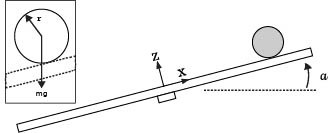
\includegraphics[width=0.7\textwidth]{sss.jpg}
\caption{Schematic representation of the Ball and Plate System (BPS).}
\end{figure}
\subsection{Euler-Lagrange approach}
In this section, the mathematical model of BPS is developed based on the Euler–Lagrange equation \cite{nokhbeh2011modelling}.
The relation between the kinetic and the potential energy
possessed by the mechanical system is described by the following
equation.

\begin{equation}
L(q_i, \dot{q_i}, t) = T( \dot{q_i}, t) - V( q_i, t) 
\end{equation}
where $L $ is the Lagrangian function which represents the
difference between the overall kinetic energy $T$ and the overall potential
energy $V$. Then, the general Euler–Lagrange’s equation is
defined as:
\begin{equation}
\dv{t} \pdv{T}{\dot{q_i}} - \pdv{T}{q_i} + \pdv{V}{q_i} = Q_i    
\end{equation}
Equation (3.2) can express the motion of a wide variety of
mechanical systems where Qi represents the i-th generalized composite force acting on the system and qi is i-th generalized coordinate.\\

The system has 4 degrees of freedom therefore four generalized coordinates; two in ball motion \([x,y]\) and two in the inclination of the plate\([\alpha, \beta]\). Here we assume the generalized coordinates of the system to be $x$ and $y$ ball’s position on the plate and $\alpha$ and $\beta$ the inclination of the plate 
\[ q_i \in \{ x,y,\alpha,\beta\}  \]
The kinetic energy of the system consists of the kinetic energy of the ball and the kinetic energy of the plate
\begin{equation} T  = T_b + T_p  \end{equation}
While the kinetic energy of the ball consists of rotational with respect
to its center of mass and translational parts:
\begin{equation}T_b  = T_{trans} + T_{rot}  \end{equation}
 The translational energy of the ball can be described by: 
\begin{equation} T_{trans} = \frac{1}{2}m_b(v^2) = \frac{1}{2}m_b(\dot{x}^2 +\dot{y}^2)   \end{equation}
 The rotational energy of the ball :
\begin{equation}T_{rot} = \frac{1}{2}J_b\omega^2 = \frac{1}{2}J_b\frac{v^2}{r^2} = \frac{1}{2}\frac{J_b}{r^2}(\dot{x}^2 +\dot{y}^2)  \end{equation}
 

Where $m_b$ is mass of the ball and $J_b$ is moment of inertia of the ball; $\dot x$ and $\dot y$ are ball’s translational velocities along x-axis and y-axis; $\omega_x$ and $\omega_y$ are ball’s
rotational velocities along x-axis and y-axis that 
\begin{equation}
\omega_y = \frac{\dot{y}}{r_b} \quad  , \quad  \omega_x = \frac{\dot{x}}{r_b}  
\end{equation}
By substituting  (3.6) and (3.5) into equations
(3.4) we will have:
\begin{equation}
T_b = \frac{1}{2}m_b(\dot{x}^2 +\dot{y}^2) +
\frac{1}{2}\frac{J_b}{r^2}(\dot{x}^2 +\dot{y}^2) =
\frac{1}{2} \left( m_b + \frac{J_b}{r_{b}^2} \right) (\dot{x}^2 +\dot{y}^2)   
\end{equation}

the kinetic energy of the plate, by considering the ball as a point mass which is placed in ($x, y$) can be expressed as: 
\begin{equation}
T_p = \frac{1}{2} (J_b + J_p) \left( \dot{\alpha}^2 +\dot{\beta}^2 \right) + \frac{1}{2} m_b \left( x\dot{\alpha} + y\dot{\beta} \right)^2 
\end{equation}
From $T_b$ (3.8) and $T_p$ (3.9)  we can calculate the total kinetic energy by substituting into Eqs (3.3):

  \begin{equation}
          T= \frac{1}{2} \left( m_b + \frac{J_b}{r_b^2} \right)(\dot{x}^2 + \dot{y}^2 ) + \frac{1}{2} (J_p + J_b) \left(\dot{\alpha}^2 + \dot{\beta}^2 \right) + \frac{1}{2}m_b \left(  x\dot{\alpha} + y\dot{\beta} \right)^2
  \end{equation} 
  \\
 The potential energy $V$ of the ball according to the plate center can be calculated as:
\begin{equation}
V_b = m_bgh = m_bg(x\sin{\alpha} + y\sin{\beta})  
\end{equation}
Now the Lagrangian function can be expressed using equation (3.1):

    \begin{multline}
    L = \frac{1}{2} \left( m_b + \frac{J_b}{r_b^2} \right)(\dot{x}^2 + \dot{y}^2 ) + \frac{1}{2} (J_p + J_b) \left(\dot{\alpha}^2 + \dot{\beta}^2 \right) \\ + \frac{1}{2}m_b \left(  x\dot{\alpha} + y\dot{\beta} \right)^2  -m_bg(x\sin{\alpha} + y\sin{\beta})  
    \label{aaa}
    \end{multline}

Then we derive the system's equations 

\begin{align}\label{eq:lnnonspbb}
\pdv{T}{\dot{\alpha}} = (J_p + J_b) \dot{\alpha} + m_b \left(x^2\dot{\alpha} + yx\dot{\beta}\right) \\             
\pdv{T}{\dot{\beta}} = (J_p + J_b) \dot{\beta} + m_b \left(xy \dot{\alpha} + y^2\dot{\beta}\right) 
\end{align}


\begin{align}\label{eq:lnnonspbb}
 \pdv{T}{\dot{x}} = \left(m_b + \frac{J_b}{r^2}\right)\dot{x} \\
 \pdv{T}{\dot{y}} = \left(m_b + \frac{J_b}{r^2}\right)\dot{y} 
\end{align}
\begin{align}
\pdv{T}{x} = m_b \left( x\dot{\alpha} + y\dot{\beta} \right)\dot{\alpha} , \qquad 
\pdv{T}{y} = m_b \left( x\dot{\alpha} + y\dot{\beta} \right)\dot{\beta} 
\end{align}
\begin{align}\label{eq:aa3}
 \pdv{T}{\alpha} = 0 ,\quad 
  \pdv{T}{\beta} = 0
\end{align}

\begin{align}\label{eq:lnnonspbb}
 \pdv{V}{\alpha} = m_bgx\cos{\alpha} ,\quad 
 \pdv{V}{\beta} = m_bgy\cos{\beta} ,\quad 
\pdv{V}{x} = m_bgx\sin{\alpha} ,\quad 
 \pdv{V}{y} = m_bgy\sin{\beta} 
\end{align}

From the Lagrange-Euler equation of the ball, we can write:
\begin{equation}
    \dv{}{dt} \pdv{T}{\dot{x}} - \pdv{L}{x} =(m_{b}+\frac{J_{b}}{r_{b}^{2}})\ddot{x}-m_{b}(x\dot{\alpha}+y\dot{\beta})\dot{\alpha}+m_{b}g\sin\alpha=0
\end{equation} 
\begin{equation}
\dv{}{dt} \pdv{T}{\dot{y}} - \pdv{L}{y} =(m_{b}+\frac{J_{b}}{r_{b}^{2}})\ddot{y}-m_{b}(x\dot{\alpha}+y\dot{\beta})\dot{\alpha}+m_{b}g\sin\beta=0
\end{equation}
It is important to note there are no external forces (except gravity) acting on the ball itself
$(Q_x = 0$ and $Q_y = 0)$ and there are forces in the form of torque acting on the plate and changing its inclination $(Q_{beta} = \tau_y $ and $ Q_{alpha} =\tau_x )$. 
\begin{align} \label{eq:asdf}
\dv{}{dt} \pdv{T}{\dot{\alpha}} - \pdv{L}{\alpha} = 
(J_b + J_p)\ddot{\alpha} + m_bx^2\ddot{\alpha} + 2m_bx\dot{x}\dot{\alpha}\\ \nonumber
+m_bxy\ddot{\alpha} +m_b\dot{x}y\dot{\beta} + m_bx\dot{y}\dot{\beta} - m_bg\cos{\alpha}
=\tau_x   
\end{align}

\begin{align} \label{eq:asdf}
\dv{}{dt} \pdv{T}{\dot{\beta}} - \pdv{L}{\beta} = 
(J_b + J_p)\ddot{\beta} + m_by^2\ddot{\beta} + 2m_by\dot{y}\dot{\beta}\\ \nonumber
+m_bxy\ddot{\beta} +m_b\dot{y}x\dot{\alpha} + m_by\dot{x}\dot{\alpha} - m_bg\cos{\beta}
=\tau_x  
\end{align}
So the 4 differential equations of the BPS are respectively (3.20),(3.21),(3.22),(3.23), finally we rewrite these non-linear equations so we got:
\begin{equation}
    0 =\left( m_b + \frac{J_b}{r^2} \right)\ddot{x} - m_b \left( x\dot{\alpha}^2 + y\dot{\alpha}\dot{\beta}\right) + m_bg\sin{\alpha}
\end{equation}
\begin{equation}
    0 = \left( m_b + \frac{J_b}{r^2} \right)\ddot{y} - m_b \left(  x\dot{\beta}^2 + x\dot{\alpha}\dot{\beta}\right) + m_bg\sin{\beta} 
\end{equation}
\begin{align}\label{eq:asdf}
\tau_x &= 
(J_b + J_p + m_bx^2)\ddot{\alpha}  + 2m_bx\dot{x}\dot{\alpha} +m_bxy\ddot{\beta}\\ \nonumber
&+m_b\dot{x}y\dot{\beta} + m_bx\dot{y}\dot{\beta} - m_bgx\cos{\alpha}
\end{align}
\begin{align}\label{eq:asdf}
\tau_y &= 
(J_b + J_p + m_by^2)\ddot{\beta}  + 2m_by\dot{y}\dot{\beta} +m_bxy\ddot{\alpha}\\ \nonumber
&+m_b\dot{x}y\dot{\alpha} + m_bx\dot{y}\dot{\alpha} - m_bgy\cos{\beta}
\end{align}
It can be seen that equations (3.24) and (3.25) describe the ball motion and how the acceleration of the ball depends on its position on the plate and on angles and angular velocities of the plate. Equations (3.26) and (3.27) show plate dynamics and how it depends on external torques, ball position, velocity, angular velocity and acceleration of the plate.

It is necessary to note that dynamics of the stepper motors are neglected, thus the system equations describe only the ball and plate problem. These dynamics will be added in the geometrical analysis subsection later, however  we should know that it's assumed stepper motors don’t lose any step and load doesn’t
affect their performance thus equations (3.26) and (3.27) can be neglected

Then we can transform the model into state space form, defining state variables $X=(x_1,x_2,x_3,x_4,x_5,x_6,x_7,x_8) = (x,\dot{x},\alpha,\dot{\alpha},y,\dot{y},\beta,\dot{\beta})$
and from eqs (3.24), (3.25) we can get the nonlinear BPS's state equations as follows:\\ 
\begin{equation}
\begin{bmatrix}
\dot{x_1}\\
\dot{x_2}\\
\dot{x_3}\\
\dot{x_4}\\
\dot{x_5}\\
\dot{x_6}\\
\dot{x_7}\\
\dot{x_8}\\
\end{bmatrix}
=
\begin{bmatrix}
x_2\\
\frac{m_b}{m_b+\frac{j_b}{r^2}}(x_1x_4^2+x_4x_5x_8-g\sin{x_3})\\
x_4\\
0\\
x_6\\
\frac{m_b}{m_b+\frac{j_b}{r^2}}(x_5x_8^2+x_1x_4x_8-g\sin{x_7})\\
x_8\\
0\\
\end{bmatrix}
+ 
\begin{bmatrix}
0 & 0 \\
0 & 0 \\
0 & 0 \\
1 & 0 \\
0 & 0 \\
0 & 0 \\
0 & 0 \\
0 & 1 \\
\end{bmatrix}
\begin{bmatrix}
u_x  \\
u_y  \\
\end{bmatrix}
\end{equation}



\subsection{Interpretation of terms in system equations}
In the Table no. 3.1 description of the terms in the system equation and there units
\begin{table}[h]
  \centering
  \caption{Interpretation of mathematical model terms}
  \begin{tabular}{ | m{8em} | m{20em}| m{1cm} | } 
  \hline
  parameter & description & unit \\ 
  \hline  \hline
   $m_b$& Mass of the ball & kg \\ 
  \hline
  $r_b$ & Radius of the ball & m \\ 
  \hline
  $J_b$ & Moment of inertia of the ball & kgm2 \\   
  \hline
  $J_p$ & Moment of inertia of the plate & kgm2 \\   
  \hline
  $x,y$ & Coordinates of the ball from the center of the plate & m \\ 
  \hline
  $\dot{x},\dot{y}$ & First time derivatives of coordinates which represents the transitional velocity  & ms-1\\   
  \hline
  $\ddot{x},\ddot{y}$ & Second time derivatives of coordinates which represents the transitional acceleration & ms-2\\   
  \hline
  $\alpha , \beta$ & Plate inclination angles & rad \\   
  \hline 
  $\dot{\alpha},\dot{\beta}$ & First-time derivatives of plate angles which represents the angular velocity & rads-1 \\   
  \hline  
  $\ddot{\alpha},\ddot{\beta}$ & Second-time derivatives of plate angles which represent the angular acceleration & rads-2 \\   
  \hline  
  $\tau$ & Torques acting on the plate & Nm \\   
  \hline
  $g$ & Gravitational acceleration  & M/s2 \\  
  \hline
  $ m_b ( x\dot{\alpha}^2+y\dot{\alpha}\dot{\beta})$ & Centrifugal force  & N \\  
  \hline
  $(J_b+J_p+m_bx^2)\ddot{\alpha} $ & Gravitational acceleration  & Nm \\  
  \hline
  $ 2m_bx\dot{x}\dot{\alpha}$ & Coriolis influence   & Nm \\  
  \hline
  $m_bgx\cos{\alpha}$ & Gravitational influence  & Nm \\  
  \hline
  \end{tabular}

\end{table}

\section{Linearization and simplfication}

To simplify and linearize the model, four main assumptions was made 
\begin{enumerate}
    \item the stepper motors don’t lose any step and load doesn’t affect their performance.
    \item The ball is assumed to be a homogenous and solid sphere
    \item The rate of change of angles is close to zero.
    \item The angles of the plate are assumed to change in range 〈-15; 15〉 or in other words, $|\alpha| < 1$ and $|\beta| < 1$ in radians.
\end{enumerate}
In the interest of model simplification, the first assumption is made that stepper motors exhibit no step loss, and the impact of the load on their performance is discounted. Consequently, angles $|\alpha|$ and $|\beta|$ are deemed direct inputs to the system. Accordingly, equations (3.26) and (3.27) may be excluded and neglected from consideration as we said before.

Secondly to find the $\frac{m_b}{m_b+\frac{j_b}{r^2}}$ term we assumed the ball to be a  solid sphere, to find  $(J_b)$ of this sphere the approximate expression for a moment of inertia of a solid ball $(J_b)$ can be derived by summing the moments of fragile disks about z-axis as can be seen in fig. 3
\begin{figure}[h]
\centering
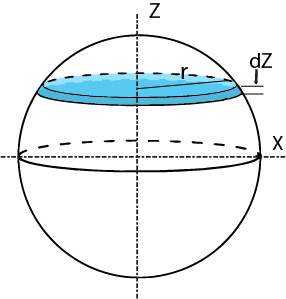
\includegraphics[width=0.4\textwidth]{SolidBallSegments.jpg}
\caption{Illustration of the moment of inertia calculation for solid ball segments}
\end{figure}
The moment of inertia expression for one disk $dJ$ derived by:
\begin{equation}
dJ = \frac{1}{2} r^2 dm = \frac{1}{2}r^2pdV = \frac{1}{2}r^2p\pi r^2dz 
\end{equation}
the mass of the disk $dm$ can be represented as the density of the ball $p$ times the volume of the disk $dV$, the volume can be represented as the disk area multiplied by the height $dz$.
To find the sum of the moment of inertia for all disks we integrate both sides of the equation to become:
\begin{equation}
J = \frac{1}{2}p\pi \int_{-R}^{R} r^4 \,dz \ = \frac{1}{2}p\pi \int_{-R}^{R} (R^2-z^2)^2 \,dz \ = \frac{8}{15} p\pi R^5 \end{equation}

 Where R is the Radius of the sphere and $y = (R^2-z^2)$ is derived from the Pythagorean theorem.
 Substituting the density expression $p = \frac{M}{V} = \frac{M}{\frac{4}{3}\pi R^3}$ gives:
\begin{equation}
J = \frac{8}{15}\left[  \frac{M}{\frac{4}{3}\pi R^3} \right]\pi R^5 
\end{equation}

 \begin{equation}
J = \frac{2}{5}MR^2 
\end{equation}
 So, as has been proven the approximate moment of inertia value for a solid ball is $J_b = \frac{2}{5}MR^2$, therefore by taking the account of all simplfications and substituting (3.32) into the system model we get:
\begin{equation}
\begin{bmatrix}
\dot{x_1}\\
\dot{x_2}\\
\end{bmatrix}
=
\begin{bmatrix}
x_2\\
\frac{5}{7}(-g\sin{x_3})\\
\end{bmatrix}
+ 
\begin{bmatrix}
0 \\
1 \\
\end{bmatrix}
\begin{bmatrix}
u_x  \\
\end{bmatrix}
\end{equation}

\begin{equation}
\begin{bmatrix}
\dot{x_5}\\
\dot{x_6}\\
\end{bmatrix}
=
\begin{bmatrix}
x_6\\
\frac{5}{7}(-g\sin{x_7})\\
\end{bmatrix}
+ 
\begin{bmatrix}
0  \\
1  \\
\end{bmatrix}
\begin{bmatrix}
u_y  \\
\end{bmatrix}
\end{equation}

It is assumed that the ball is rolling without slipping in continuous contact with the plate keeping in mind the rate of change of angles is low and close to zero, and because of that the angular velocity and the acceleration of the the plate rotation will be very low and can be negligible,
\[ \dot{\alpha} \approx 0 \]\[ \dot{\beta} \approx 0  \]

the last assumption to finally linearize the model is that the angle of inclination for the plate is relatively small (up to ± 15) which leads $\longrightarrow  \sin{\alpha} \simeq \alpha, \, \sin{\beta} \simeq \beta$ in rads so the final linearized equation will be
\begin{equation}    
\begin{bmatrix}
\dot{x_1}\\
\dot{x_2}\\
\end{bmatrix}
=
\begin{bmatrix}
x_2\\
0\\
\end{bmatrix}
+ 
\begin{bmatrix}
0 \\
\frac{5}{7}(-g) \\
\end{bmatrix}
\begin{bmatrix}
\alpha \\
\end{bmatrix}
\end{equation}

\begin{equation}
\begin{bmatrix}
\dot{x_5}\\
\dot{x_6}\\
\end{bmatrix}
=
\begin{bmatrix}
x_6\\
0\\
\end{bmatrix}
+ 
\begin{bmatrix}
0  \\
\frac{5}{7}(-g)  \\
\end{bmatrix}
\begin{bmatrix}
\beta  \\
\end{bmatrix}
\end{equation}

Equation No. (3.35) serves as the foundational equation for the subsequent steps in our process. Following these simplifications, the system equations can be expressed in transfer function form:
\begin{equation}\ddot{x} +\frac{5}{7}g \alpha = 0 \end{equation}
\begin{equation}\ddot{y} +\frac{5}{7}g \beta = 0 \end{equation}
Assuming the angles as inputs to BPS, the linearized transfer function can be obtained as:
\begin{equation}     G(s) = \frac{x(s)}{\alpha(s)} = -\frac{5}{7}\frac{g}{s^2} \end{equation}
\begin{equation} G(s) = \frac{y(s)}{\beta(s)} = -\frac{5}{7}\frac{g}{s^2} \end{equation}

To validate our linearization process, we compared the linear model with non-linear simulink and Simscape models through an open-loop step response by the Simulink program, using four different inputs, as presented in Figure 3.4. Since the system is open-loop, the response is unstable, and we can also notice from the figure that the difference between the three models increases as the angle of the plate \(\alpha\) increases. This is due to our assumption that the input angle changes in the range 〈15; 15〉.

\begin{figure}[h]
    \centering
    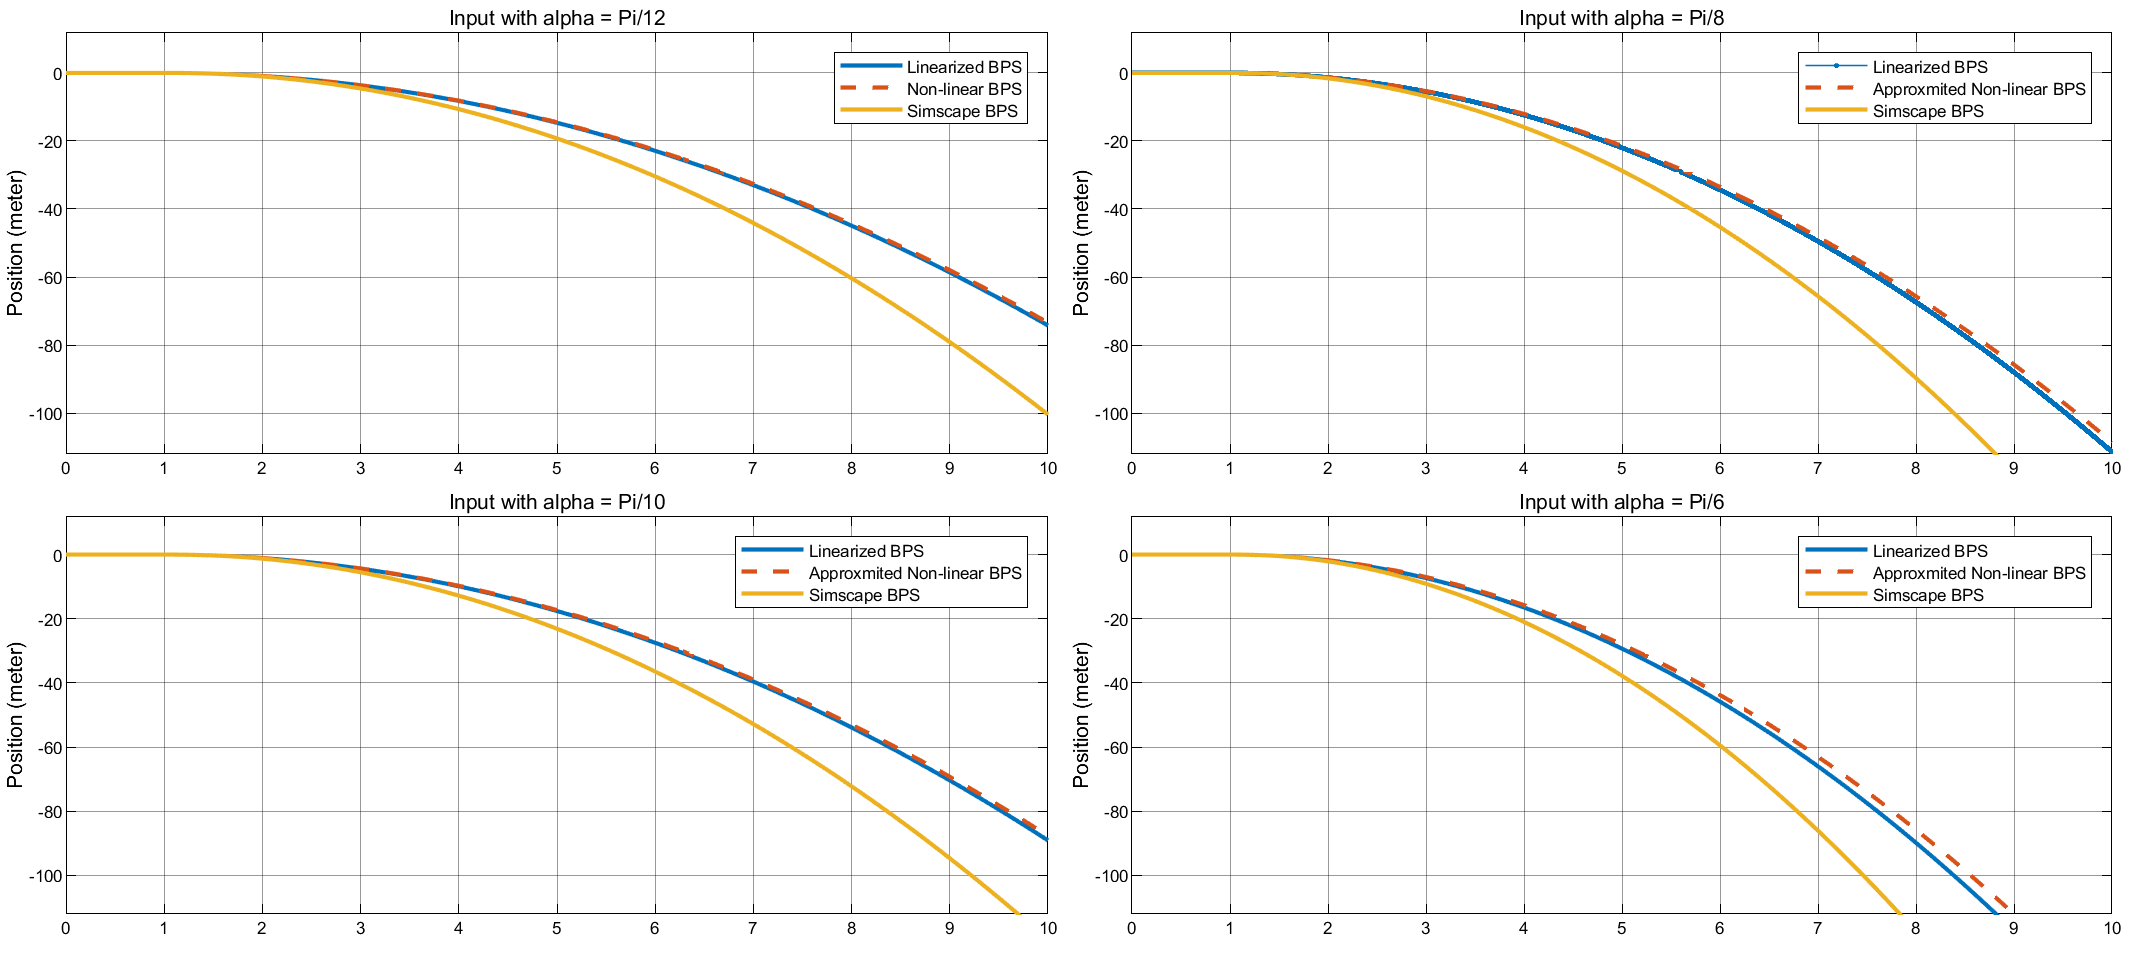
\includegraphics[width=1\textwidth]{Openl_loop_response_of_BPS_for_contant angle}
    \caption{Comparison of open-loop responses for linear, non-linear, and Simscape BPS models}
\end{figure}

\section{Geometrical analysis}
Since our overall system input should be the angle signal provided to the servo motor, not the plate inclination angle itself, we should discover the transfer function of the servo motor and then we should determine the gain or geometrical relationship between the plate inclination angle and servo motor angle
\subsection{Servo motor modeling}
Servomotors, like the MG995 model that we used in our thesis, are widely used for precise linear or angular motion in engineering. In Fig. 3.5, key components of the MG995 are highlighted. The DC motor generates rotational motion from applied voltage, while the gearbox adjusts speed and boosts torque. The electronic control board interprets PWM signals, converts them to angles, and computes control signals by comparing them with the current angle. Unlike professional servos with encoders, inexpensive hobby servos, including china made MG995's, often lack encoders and instead use a potentiometer for position sensing. The potentiometer, rotating with the output shaft, induces a voltage signal variation sent to the control board. This signal goes as a feedback and helps the internal controller calculate the difference between the desired and current positions, serving as the input for the embedded controller \cite{santanacob}.
\begin{figure}[h]
    \centering
    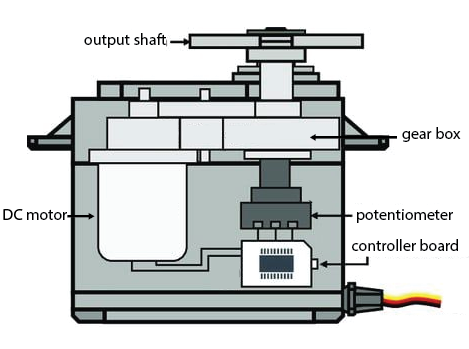
\includegraphics[width=0.5\textwidth]{servomotor_schematic.png}
    \caption{Schematic representation of key components in the MG995 servomotor}
\end{figure}
In the electrical dynamics of Fig. 3.6, key parameters include \(u\) (voltage applied), \(i\) (electrical current), \(R\) (motor resistance), \(L\) (inductance), and \(e\) (back electromotive force). On the mechanical side, \(\tau_m\) denotes motor torque, \(\tau_{jm}\) is motor moment of inertia, \(b_m\) is viscous friction coefficient, \(\tau_f\) is viscous friction torque, \(\theta_m\) is motor shaft rotation angle, N is gearbox gear ratio, \(J_l\) is load moment of inertia, \(\tau_l\) is load torque, and \(\theta_l\) is servo output shaft rotation angle.
\begin{figure}[h]
    \centering
    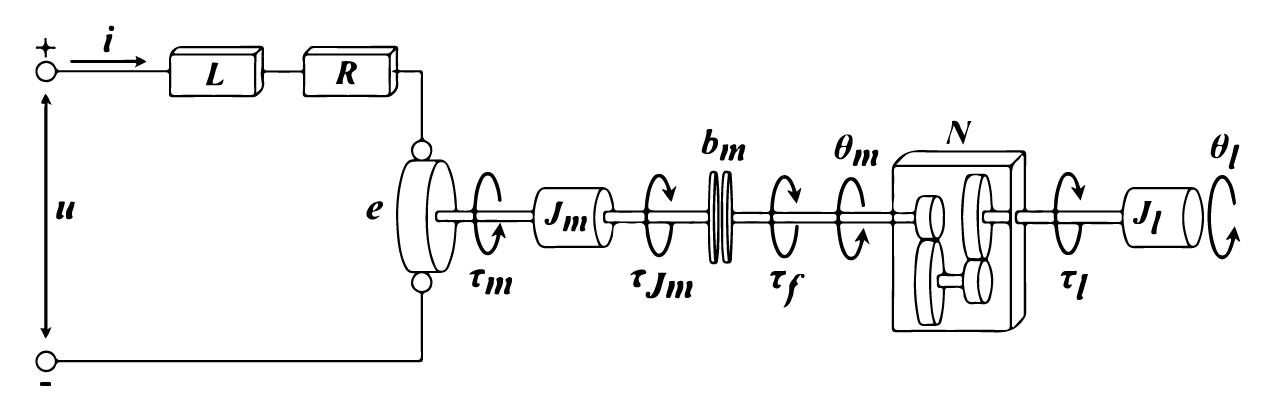
\includegraphics[width=0.8\textwidth]{Servomotor_dynamical_diagram}
    \caption{The electromechanical diagram of a servomotor system}
\end{figure}
 To obtain a transfer function that represents the open-loop dynamics $P(s)$ of a servo motor for a voltage input $U(s)$ and as output the angle of the servo output shaft $\Theta_l(s)$, is given by:

\begin{equation}P(s) = \frac{\Theta_l(s)}{U(s)} = \frac{K_t K_\omega \eta}{(J_{eq}s^2 + b_{eq}s)}
\end{equation}

 where $K_t$ is the motor torque constant, $K_\omega$ is the speed constant, and $\eta$ is the gearbox efficiency factor, $J_{eq} = J_l + J_m\eta N^2$ and $b_{eq} = b_m\eta N^2$. This transfer function characterizes the open-loop behavior of the servo motor.\\
\begin{figure}[h]
    \centering
    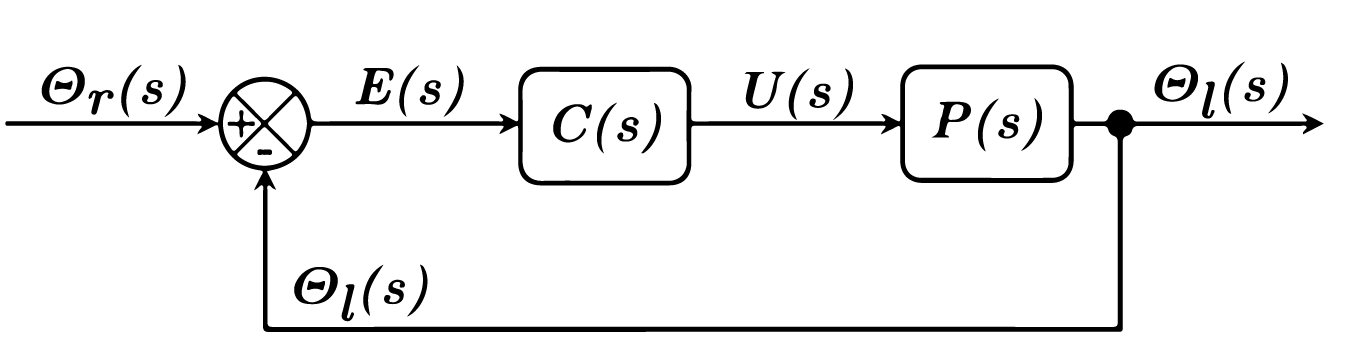
\includegraphics[width=0.6\textwidth]{servomotor_closed_loop_diagram}
    \caption{Diagram illustrating the key parameters in the dynamical model of the servomotor}
\end{figure}
The closed-loop system is shown in Figure 3.7, where the controller $C(s)$ is assumed to use a proportional control with gain $K_P$. The input of the closed-loop control is the commanded angle $\Theta_r(s)$, and the feedback signal is the load output shaft angle $\Theta_l(s)$. The error signal $E(s)$ is defined as the difference between the commanded angle and the actual output angle. The open-loop transfer function $P(s)$, is used to obtain the closed-loop transfer function $G(s)$, which relates the output angle $\Theta_l(s)$ to the commanded angle $\Theta_r(s)$:

\begin{equation} 
G(s) = \frac{\Theta_l(s)}{\Theta_r(s)} = \frac{\eta K_t K_P}{(RJ_{eq}s^2 + (Rb_{eq} + \eta N^2 K_t^2 K_P)s + \eta N K_t K_P)} 
\end{equation}

This transfer function characterizes the closed-loop behavior of the servo motor, taking into account the effects of the proportional control and the feedback loop.
Due to the limited time in our thesis we will use the parameters and transfer function identified in\cite{santanacob} which it uses a very unique method to determine the input and output angles of the servo therefore to be able to use the Matlab system identification toolbox:

\begin{equation} \frac{\Theta_l(s)}{\Theta_r(s)} = \frac{224.8}{s^2 + 22.33s + 225.4} 
\end{equation}
can also be represented in state space formula as:
\begin{equation}
\begin{bmatrix}
\Dot{\Theta_l}\\
\Ddot{\Theta_l}\\
\end{bmatrix}
=
\begin{bmatrix}
1\Dot{\Theta_l}\\
225.4\Theta_l + 22.33\dot{\Theta_l}\\
\end{bmatrix}
+ 
\begin{bmatrix}
0  \\
224.8 \\
\end{bmatrix}
\begin{bmatrix}
\Theta_r  \\
\end{bmatrix}
\end{equation}

\subsection{Linking Plate Inclination and Servo Motion}
There are several different ways to connect the motor to the plate that to convert the rotational move of the servomotor into a simple plate inclination, we have adopted the simplest method, such as the one shown in figure. 3.8, by the requirement of minimum inclination angle and due to the lack of availability of all parts in the market, we were able to obtain and construct the dimension shown in Table. 2 \\
\begin{figure}[h]
    \centering
    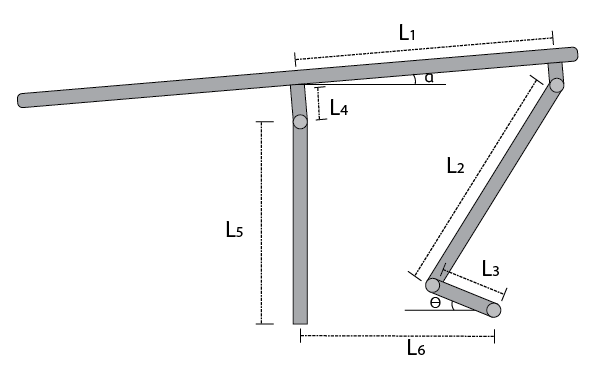
\includegraphics[width=0.8\textwidth]{actutation_platform_geometry.png}
    \caption{geometric illustration of the linkage between actuator and the plate of BPS}
\end{figure}

\begin{table}[h]
  \centering
  \caption{System dimensions in centimeter}
  \begin{tabular}{|c|c c c c c c|}
    \hline
    \hline
     X & L1 & L2 & L3 & L4 & L5 & L6 \\
    \hline
    Value & 9.5 & 24 & 1.5 & 5 & 22 & 13.4 \\
    \hline
    \hline
     Y & L1 & L2 & L3 & L4 & L5 & L6 \\
    \hline
    Value & 10 & 24 & 1.5 & 5 & 22 & 13 \\
    \hline
  \end{tabular}
\end{table}
The relation between the angle of rotation of the plate around the x axis \(\alpha\) and the angle of rotation of servomotor arm L3 \(\Theta\) is:
\begin{equation}
\sin{\Theta} = \frac{L_3}{L_1}\sin{\alpha}
\end{equation}
which can be represented as a constant gain \(K_l= \frac{L_3}{L_1}\), from Table. 2
\begin{equation}
K_{lx} = 0.158 \\\
K_{ly} = 0.150
\end{equation}
but the behaviour of the angles appears a Little different so we decided to map the inclination angle with the servo motor angle and determinee by the linear relationship regression the appropriate gain
the full table and details of mapping method found in Appendix C, and the new gain values we get is:
\begin{equation}
K_{lx} = 0.0445 \\\
K_{ly} = 0.0377
\end{equation}
The overall system equation taking in account the plant equation Eq. (3.39) (3.40) with the linkage gain Eq. (3.47) and the identified servomotor equation Eq. (3.43) can be represented as follows:
\begin{equation}
\frac{x}{\Theta_r}=\frac{70.1}{s^4+22.33s^3+225.4s^2}
\end{equation}
Which after state space transformation:
\begin{equation}
\begin{bmatrix}
\Dot{x_1}\\
\Ddot{x_2}\\
\Dot{x_3}\\
\Ddot{x_4}\\
\end{bmatrix}
=
\begin{bmatrix}
x_1\\
\frac{-5}{7}gx_3\\
x_4\\
-225.4x_x -22.33x_4\\
\end{bmatrix}
+ 
\begin{bmatrix}
0  \\
0 \\
0 \\
70.1
\end{bmatrix}
\begin{bmatrix}
\Theta_r  \\
\end{bmatrix}
\end{equation}
The system in Eq. (3.47)(3.48) is a fourth order transfer function, unstable due to the two poles in the origins as shown fig. 3.9, however it can be considered as a second order system since the other two poles in fig. 3.9 are in the left side far away from the origin so they have a little impact on the system behavior

\begin{figure}[h]
    \centering
    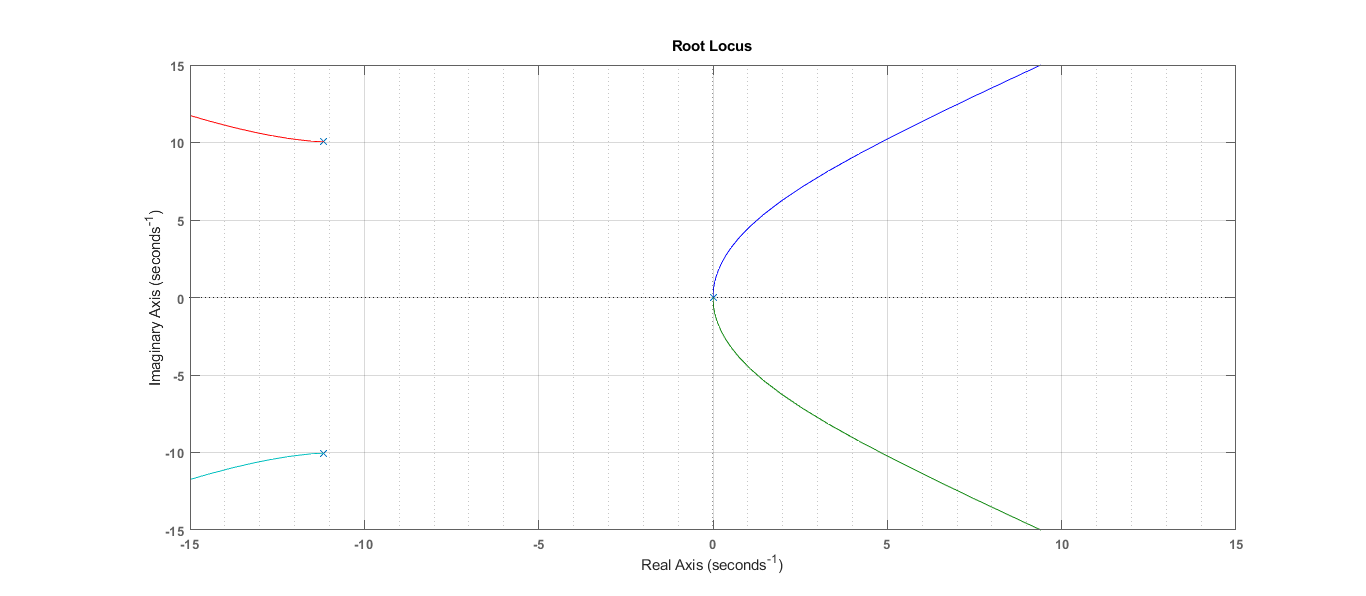
\includegraphics[width=1\textwidth]{RootLocus.png}
    \caption{Root Locus Analysis: Navigating Stability for BPS}
\end{figure}



\chapter{Controller Design Approaches}
\graphicspath{ {Figures/chapter04} }
In this chapter we will focus on designing an appropriate controller theoretically and experimentally 
\section{System Requirements}
Before starting into the evaluation of the controller's performance, certain requirements conditions and specifications have been identified as crucial benchmarks. These prerequisites provide a foundational base  to be able to determine if the controller performs well enough:

\begin{enumerate}
\item the plate to incline only in \(15\deg\) in both coordinates.
\item Settling time less than 5 seconds (\(Ts < 5\))
\item Rise time less or equal to 1 seconds (\(T_r < 0.5\)).
\item A overshoot less than 20\% (\(M < 0.20\)).
\item The static error should be equal to zero or less than 25 pixels (\(e_0 < 0.05\)).
\end{enumerate}
The goal is that the controller will be able to fulfill these demands.

\section{System Controllability and Observerability}
The controllability and observability of the system are crucial aspects in ensuring effective control. In order to have full freedom in the placement of the poles, it is necessary to check the controllability of the system. This is done by determining the controllability matrix $S$ \cite{nise2020control}, which is given by:
\begin{equation}
S = \begin{bmatrix}
B & AB & A^2B & \dots & A^{n-1}B
\end{bmatrix}
\end{equation}
where $n$ is the number of states. If the determinant of the matrix $S$ is non-zero, it indicates that the placement of the poles is not restricted, allowing for the fulfillment of control demands.
Using the overall plant transfer function in Eq. (3.48), The determined controllability matrix:
\begin{equation}
   S = 1.0 \times 10^5 \times
    \begin{bmatrix}
        0 & 0 & 0 & -0.0158 \\
        0 & 0 & -0.0158 & 0.3527 \\
        0 & 0.0023 & 0.0010 & 0.6159 \\
        0.0023 & -0.0503 & 0.6159 & -2.4073 \\
    \end{bmatrix} 
\end{equation}
The rank of the controllability matrix Eq.(4.2) for the linear model is 4, which is full rank meaning the system is completely controllable


Observability is equally important, as the controller needs to have all the information to control the system successfully. The observability of the system can be checked using the observability matrix $O$, defined as:
\begin{equation}
   O = 
\begin{bmatrix}
    C \\
    CA \\
    CA^2 \\
    \vdots \\
    CA^{n-1}
\end{bmatrix}
\end{equation}

Just like in controllability, if the observability matrix Eq.(4.4) is full rank then the system is observable.
\begin{equation}
   O = 
\begin{bmatrix}
    1.0000 & 0 & 0 & 0 \\
    0 & 1.0000 & 0 & 0 \\
    0 & 0 & -7.0071 & 0 \\
    0 & 0 & 0 & -7.0071 \\
\end{bmatrix}
\end{equation}
Since the matrix O is full rank (rank(O) = 4). This
means that we can estimate all the states from the displacement measurement and the system is both observable and controllable

\section{PID Controller design}
The Proportional Integral Derivative (PID) controller is one of the most widely used controllers today. The ideal PID controller is described by the equation:
\begin{equation}
u(t) = K_P e(t) + K_I \int_0^t e(\tau) d\tau + K_D \frac{d}{dt} e(t)
\end{equation}
where \(u\) represents the control signal and \(K_p\) , \(K_I\) and \(K_D\) denote the proportional, integral and derivative gains respectively. Notably large value for \(K_p\) leads to increased speed of the controller. However, it can compromise stability. \(K_I\) 
eliminates static error, but also decreases stability. On the other hand the derivative gain, \(K_D\), decreases the oscillation and leads to stability enhancement 
The closed-loop transfer function of a PID-controlled system is given by: Eq.4.2 where s is the Laplace variable
\begin{equation}
G_c(s) = K_P + \frac{K_I}{s} + K_Ds 
\end{equation}
To enable the PID controller's operation, the error \(e(t)\) is essential. This error is derived by taking the difference between the reference signal \(r(t)\) and the actual system output \(x(t)\)), represented as the variance between the desired position  and the sensed position (as depicted in Fig. 4.1). In this illustration, two feedback loops are evident. The internal loop corresponds to the servomotor's internal controller, managing its own dynamics. Simultaneously,  and the external loop ensures that the PID controller receives the necessary input after error calculation
\begin{figure}[h]
    \centering
    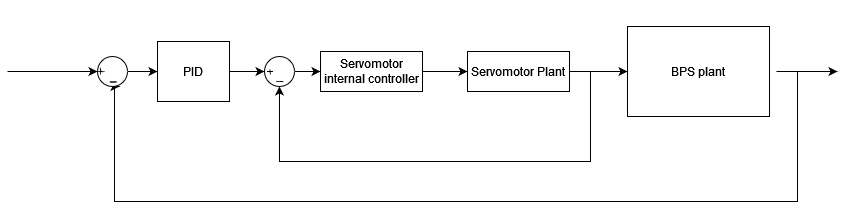
\includegraphics[width=0.95\linewidth]{PID_digram.png}
    \caption{A block diagram illustrates BPS's control mechanism using PID}
    
\end{figure}

In real-world scenarios, achieving an optimal PID controller often involves considering the inherent dynamics and characteristics of the system. Practical tuning methods, such as frequency response analysis or model-based approaches, provide engineers with tools to fine-tune the controller parameters for specific performance criteria. In order to meet our requirements, we utilized the Simulink PID block tuner tool. The block diagram, as depicted in Fig. 4.2, served as the foundation for our tuning process.

\begin{figure}[h]
    \centering
    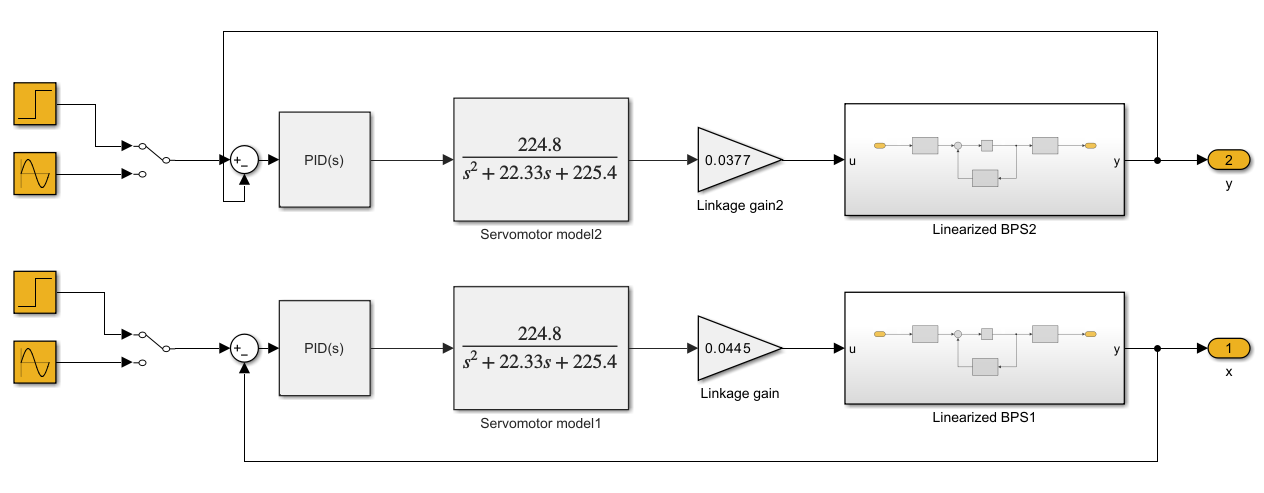
\includegraphics[width=0.95\linewidth]{idealPID.png}
    \caption{the simplified Simulink PID diagram, highlighting its key components and signal pathways}
    
\end{figure}

Although our tuning efforts using the Simulink PID block tuner tool yielded a very good response, we faced some challenges that required attention. The main concern was the PID output,  went beyond the 0 to 180-degree range. This presented a practical issue as the servo couldn't handle values outside its normal operational limits.

Moreover, our sensor provided the ball position through an analog signal ranging from 0 to 1024, making it necessary to make adjustments to the model. To resolve these issues, we implemented a saturation function to limit the PID output within a manageable range. Additionally, we introduced a calibration transformation and filter to the sensor signal. To account for calculation and data transmission delays, we incorporated a delay component into the model.

These adjustments and refinements led us to the development of Fig. 4.3, which represents a more practical and realistic model (a higher quality image can be found in appendix B). This modified model takes into account the limitations and characteristics of both the servo and the sensor and considers the calculation and data transport delay from the computer to the arduino and vice versa.

\begin{figure}
    \centering
    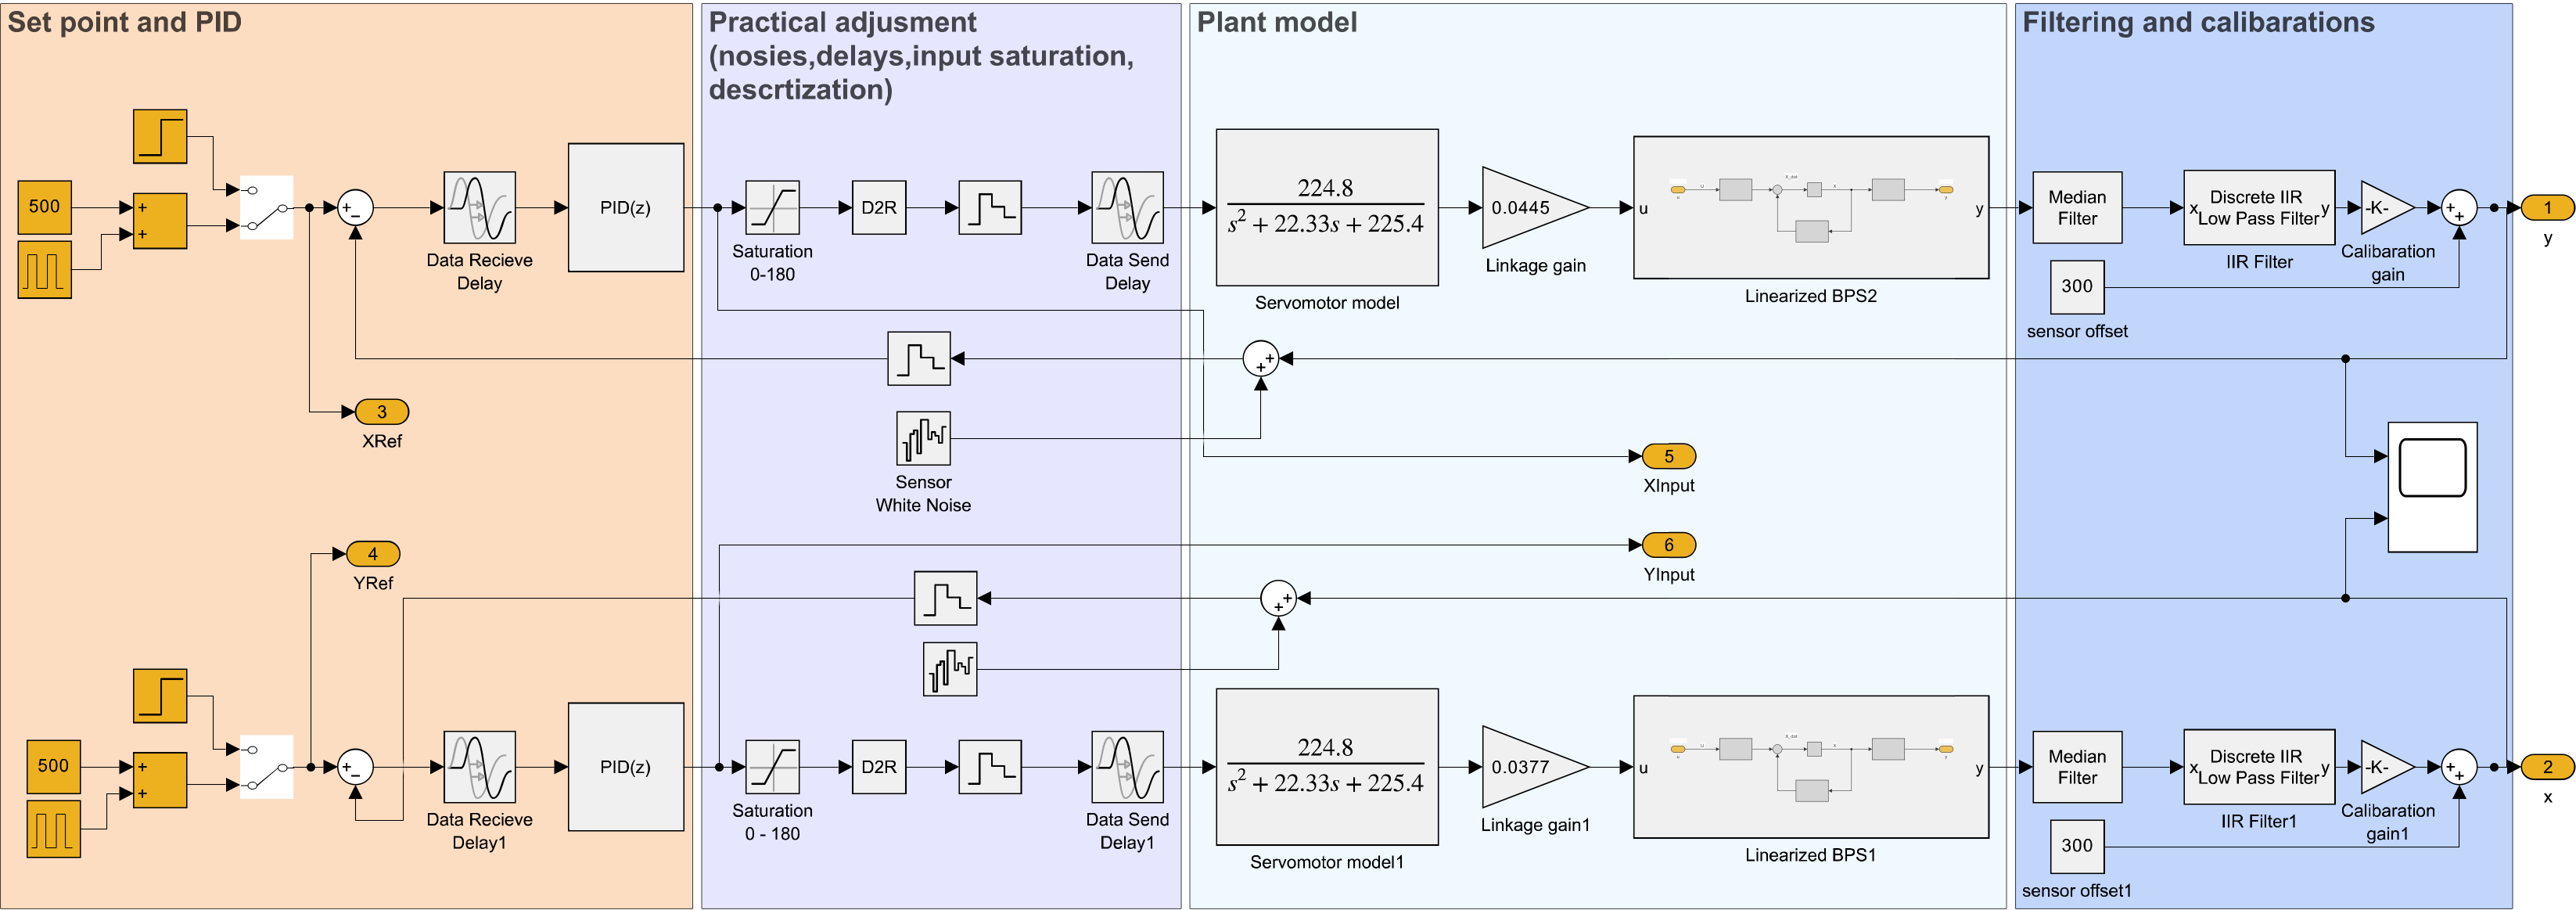
\includegraphics[width=1\textwidth]{practicalPID.png}
    \caption{Refined Simulink Model Illustrating Practical Adjustments}
    
\end{figure}
As a result of these adjustments introduced complexity and non-linearity to the system that surpassed the capabilities of SIMULINK tuning tools. Consequently, we shifted to a manual tuning approach, relying on a trial-and-error method to iteratively fine-tune the parameters for optimal system performance. 
The PID gains, determined through manual tuning using a trial-and-error method, are summarized in Table 1.

\begin{table}[h]
    \centering
    \caption{Tuned PID Parameters}
    
    \begin{tabular}{|c|c|c|c|}
        \hline
        &
        \text{Proportional Gain (\(K_P\))} & 
        \text{Integral Gain (\(K_I\))} & 
        \text{Derivative Gain (\(K_D\))} \\
        \hline
        \hline
        PID X 1 & 
        \text{0.125} &
        \text{0.00184} & 
        \text{0.098} \\
        \hline
        PID Y 1 & 
        \text{0.127} &
        \text{0.00084} & 
        \text{0.088} \\
        \hline
        \hline
        PID X 2 & 
        \text{0.165} &
        \text{0.00085} & 
        \text{0.11} \\
        \hline
        PID Y 2 & 
        \text{0.167} &
        \text{0.00084} & 
        \text{0.105} \\
        \hline
        \hline
        PID X 3 & 
        \text{0.105} &
        \text{0.00084} & 
        \text{0.07} \\
        \hline
        PID Y 3 & 
        \text{0.107} &
        \text{0.00184} & 
        \text{0.069} \\
        \hline
        \hline
    \end{tabular}
\end{table}


\section{PID Controller Implementation}
After the theoretical foundation of the PID controller design, the next crucial step is its practical implementation. This section outlines the real-world application of the PID controller to control the Ball and Plate System (BPS).

\subsection{Real System Implementation}

The PID controller, designed based on the principles discussed earlier, was implemented in the physical BPS. Figure 4.4 showcases the real system setup, highlighting the integration of the PID controller into the overall system.

\begin{figure}[h]
    \centering
    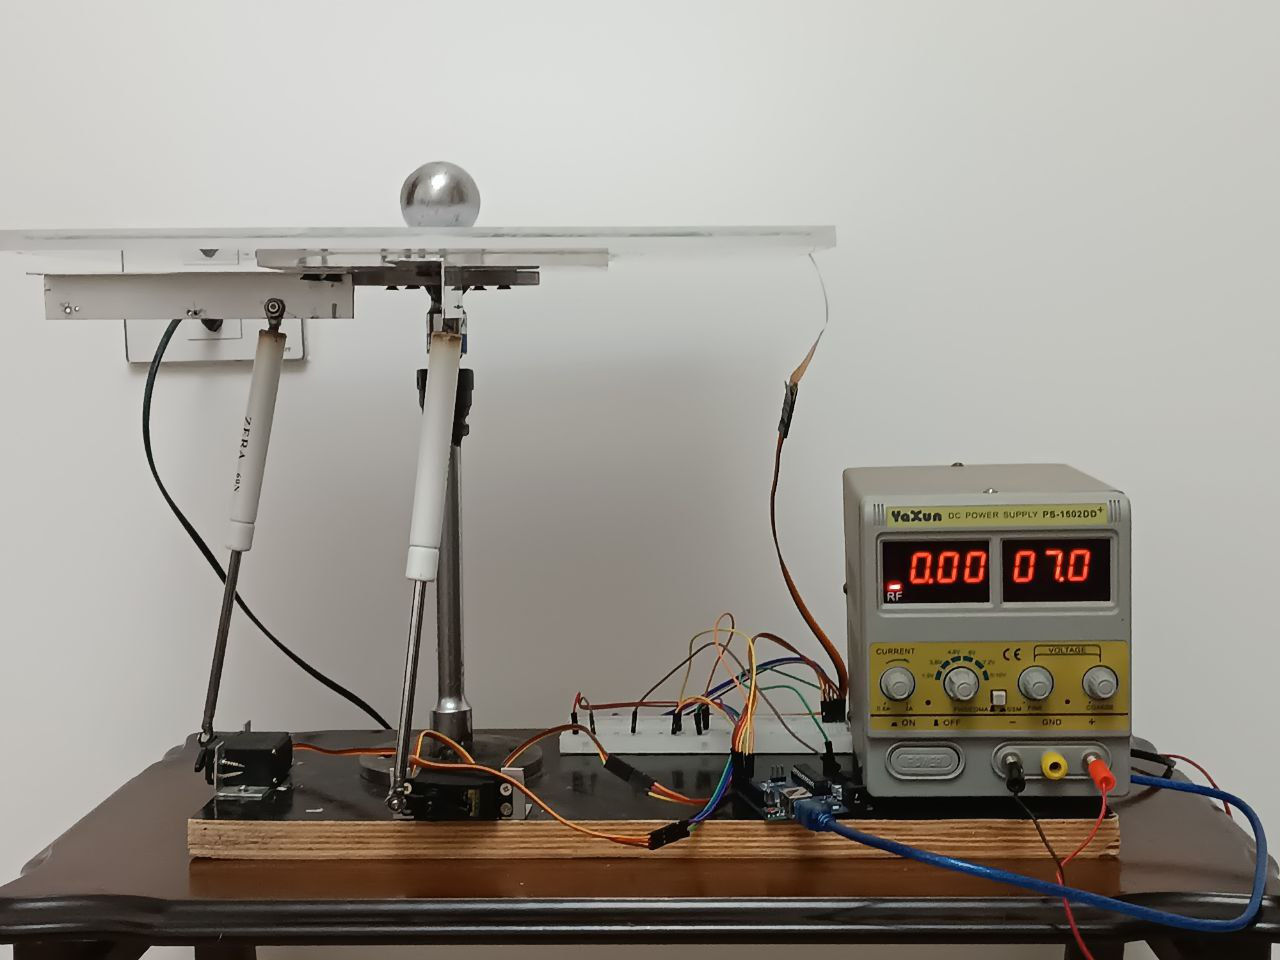
\includegraphics[width=0.95\linewidth]{real_plant.jpg}
    \caption{Real System Implementation with PID Controller}
    \label{fig:real-system-implementation}
\end{figure}

In this configuration, the PID controller interacts with the servomotors to adjust the position of the plate in response to the sensed ball position. The physical setup involves the Arduino Uno, servomotors, resistive touch screen, and the mechanical structure of the BPS.

\subsection{Simulink Model for PID Control}

To facilitate a seamless interaction between the PID controller and the real system, a Simulink model was developed. Figure 4.5 illustrates the Simulink model responsible for PID control (a higher quality image can be found in appendix B), incorporating the practical adjustments discussed earlier.

\begin{figure}[h]
    \centering
    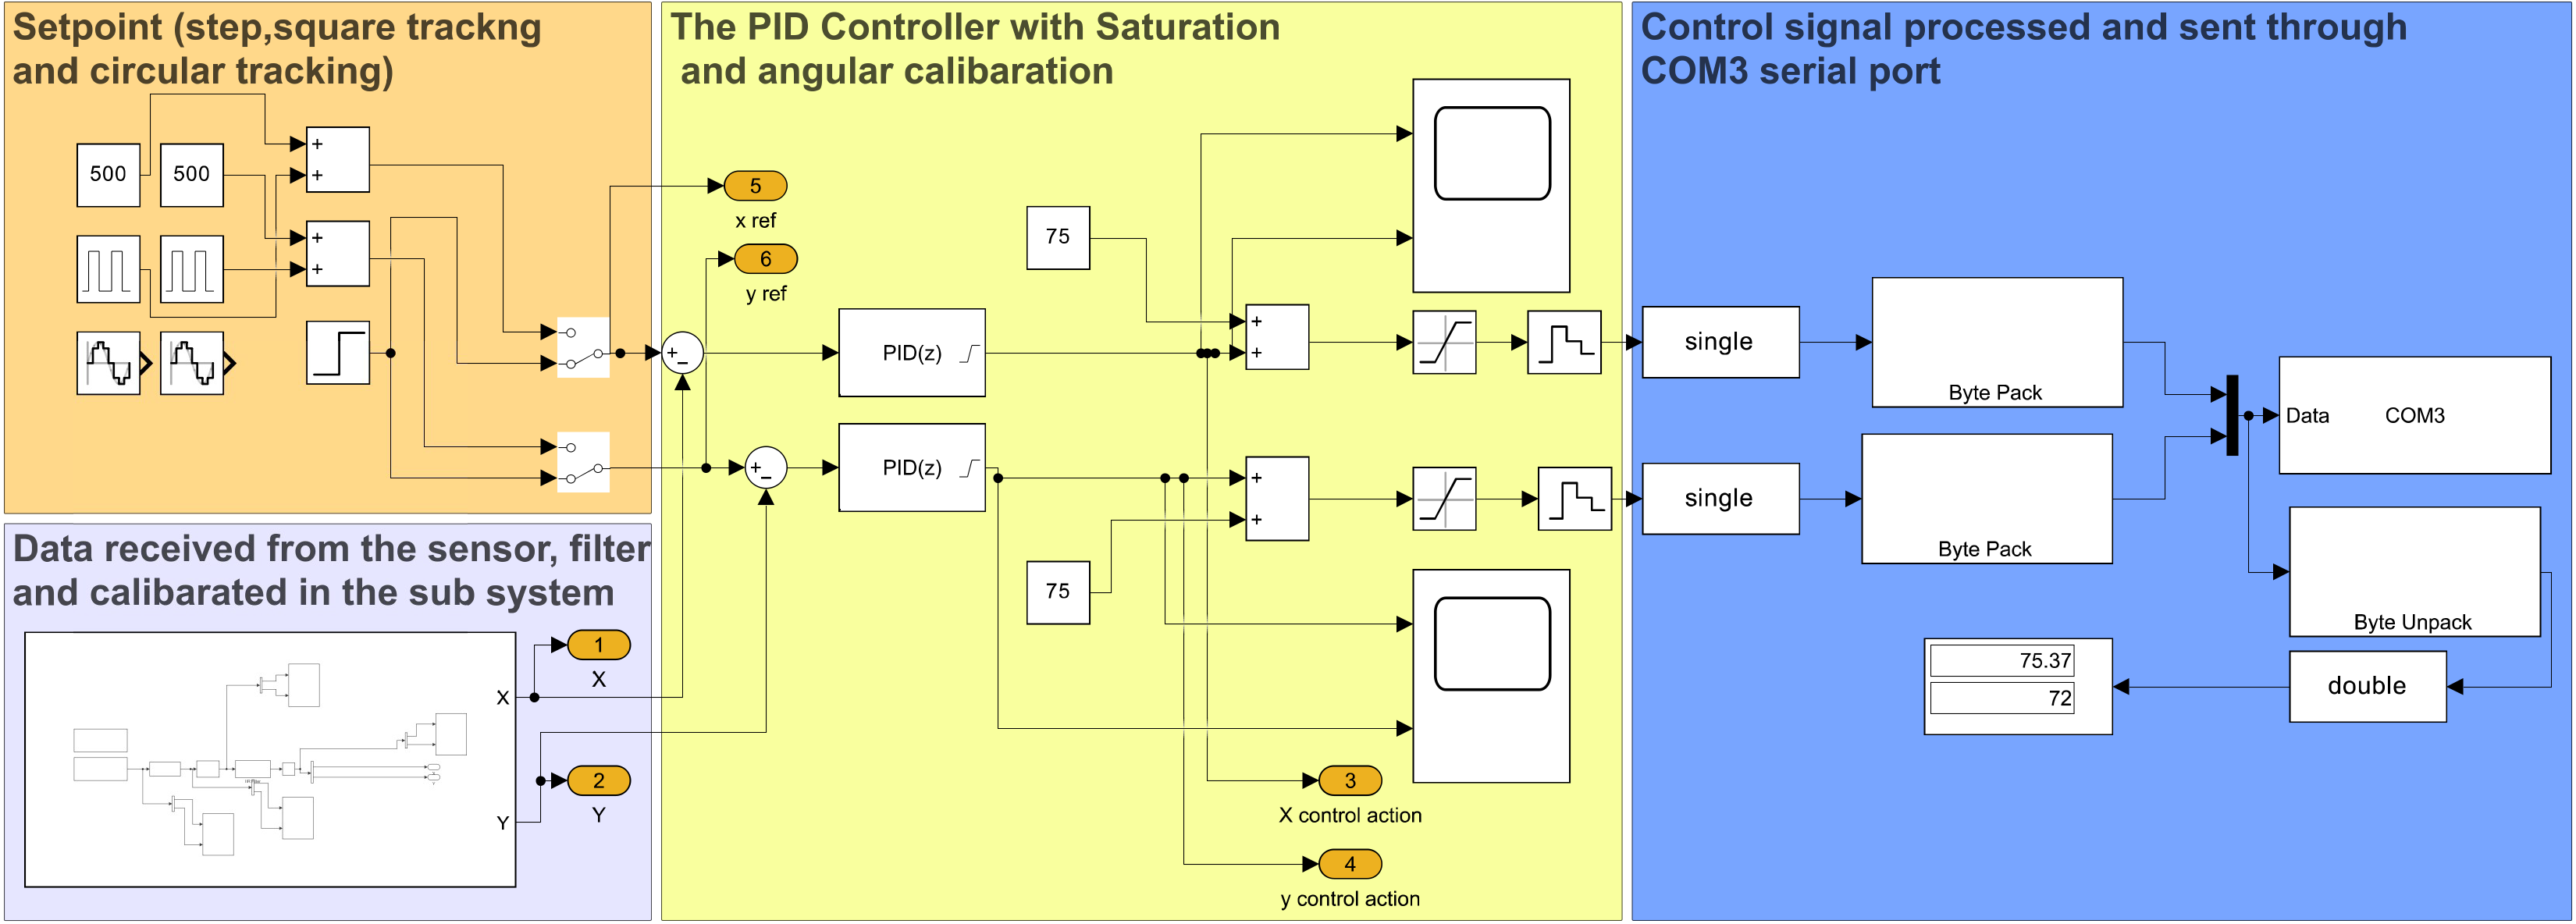
\includegraphics[width=0.95\linewidth]{simulink_real_system_pid_model.png}
    \caption{Simulink Model for PID Control Implementation}
    \label{fig:simulink-pid-model}
\end{figure}

The Simulink model integrates the PID block with the plant model, representing the dynamics of the BPS. Additionally, it includes the saturation function, calibration transformation, and filters to ensure compatibility with the real-world limitations of the servo and sensor.

The communication between the Simulink model and the real system is established through the Arduino via COM3 serial pot, which serves as the intermediary for data exchange. This bidirectional communication allows the Simulink model to receive real-time data from the system and send control signals back for continuous adjustment.

\subsection{Challenges and Manual Tuning}

Despite the theoretical foundation and simulation-based tuning, the real-world implementation presented challenges. 

One of the initial challenges was determining the appropriate time sampling for the PID controller to ensure compatibility with the Arduino. An approximate time sample for the Arduino was estimated, considering its processing capabilities, and additional delay factors were incorporated. After an iterative experimentation, it became evident that a time sample of 0.08 seconds provided the best response.the chosen time sampling is crucial for the overall responsiveness of the PID controller in the real system. It plays a pivotal role in balancing the need for rapid adjustments with the Arduino's processing constraints. This optimization contributes to achieving a smooth and stable control mechanism for the Ball and Plate System.
\begin{onehalfspacing}
Another significant challenge encountered during the real-time implementation was associated with the differential part of the PID controller. In instances where the ball experienced sudden and significant movements, resulting in rapid changes in its position, the differential component of the controller exhibited a behavior known as "differential kicks" presented in Fig. 4.6. These sudden kicks or spikes in Fig. 4.6 had a detrimental impact on the stability of the ball on the plate.


\begin{figure}[h]
    \centering
    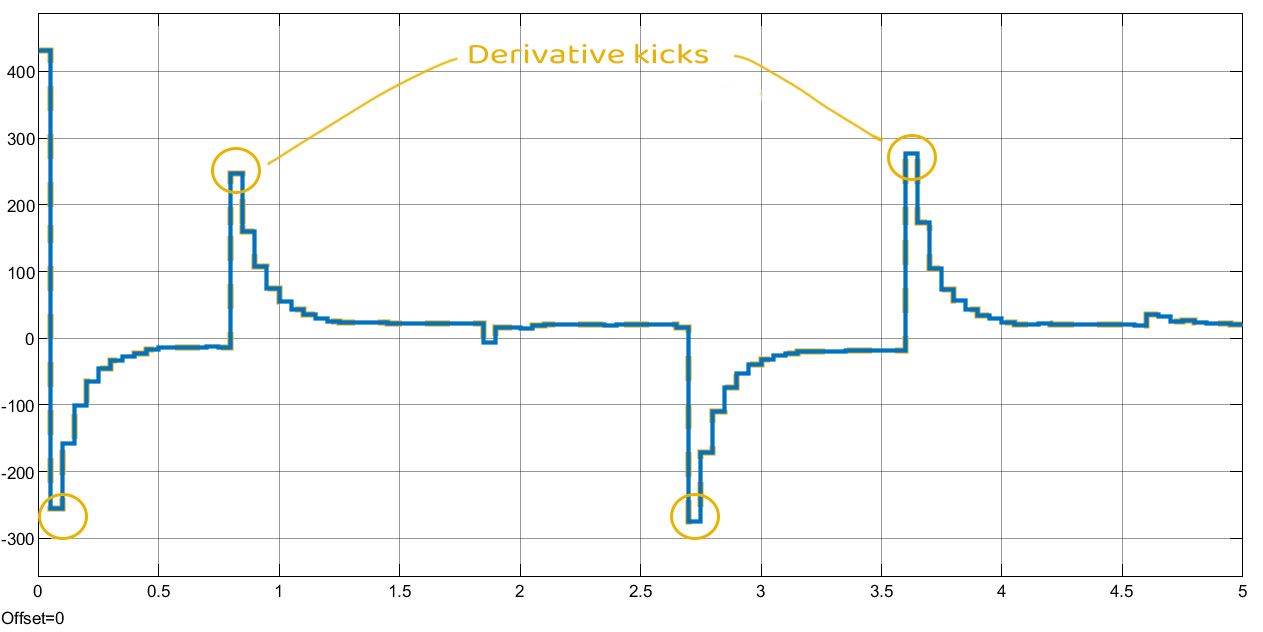
\includegraphics[width=0.75\linewidth]{Derivative_kicks.jpg}
    \caption{Illustratiion of the "Differential Kicks" Phenomenon }
    \label{fig:enter-label}
\end{figure}
To solve this issue an median filter was applied. This filter smoothed out the extreme and abrupt changes in the controller signal, ensuring a more controlled response. By computing the average controller signal over a 3 time window, this approach struck a balance between responsiveness and stability, enhancing the adaptability of the control system.
\end{onehalfspacing}


%Table 1 summarizes the tuned PID parameters obtained through manual tuning for each of the three PID controllers controlling the X and Y axes.

%\begin{table}[h]
%    \centering
%    \caption{Tuned PID Parameters for Real System Implementation}
%    \begin{tabular}{|c|c|c|c|}
%        \hline
%        & \text{Proportional Gain (\(K_P\))} & \text{Integral Gain (\(K_I\))} & \text{Derivative Gain (\(K_D\))} \\
%        \hline
%        \hline
%        PID X & 0.2 & 0.0005 & 0.1 \\
%        \hline
%        PID Y & 0.15 & 0.0003 & 0.08 \\
%        \hline
%    \end{tabular}
%\end{table}


\chapter{Results and Discussion}
\graphicspath{ {Figures/chapter05} }
\section{Introduction}
In this chapter, we'll show and confirm the outcomes of our modeling efforts, examining both the linear and non-linear states of the model. We'll compare these models with the real-world implementation and Simscape simulations. Next, we'll evaluate the performance of the PID controller we designed earlier in the previous chapter by comparing simulated results with our system actual outcomes.
\section{Open Loop Step Response of Linear and Non-linear Models against Real Implementation}
To ensure our model's accuracy, we conducted a step response comparison under Open Loop conditions, as depicted in Figure 5.1.
\begin{figure}[h]
    \centering
    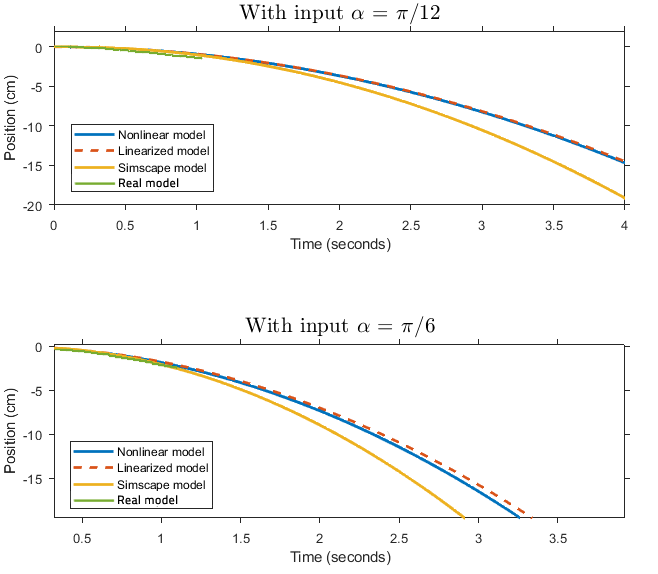
\includegraphics[width=1\linewidth]{Linearization_validation.png}
    \caption{open loop response comparison between the real plant, nonlinear model, linearized model, simscape model}
    \label{fig:enter-label}
\end{figure}
The Figure 5.1 indicate a clear instability in the system, particularly noticeable as the input angle rises. A noticeable difference arises between the linearized and non-linear systems. The observed difference can be traced back to our simplification assumption,  limiting the input plate inclination angle to the range of -15 to +15 degrees.Any variations beyond this specified range result in increased disparities between the linear and non-linear responses.

Moreover, our model assumes an infinite plate space, depicting a scenario where the ball neither falls nor bounces. This abstraction diverges from reality, introducing challenges and complexities in the practical implementation of the system

As a final test, the response of the real system to an angle of pi/12 is depicted in the figure 5.1. Notably, the response aligns reasonably well with our linear model, suggesting a certain level of reliability in our linearized representation

\section{Closed Loop Validation of PID Controller Performance}
In the tuning stage of our PID controller, achieving system stability was impossible  using only a P or PI controllers, The ball exhibited endless rolling or even falling off the plate.
therefore tuning a full PID controller was necessary, after  manual tuning process characterized by trial and error the parameter derived was  as shown in table 4.1. The resulting  experimental step responses of the three PIDs tuned parameters are depicted in Figure 5.2, and details of these responses characteristics are presented in Table 5.1, The experimental step responses in Figure 5.2 reveal distinct behaviors under the influence of PID1, PID2, and PID3. PID2, characterized by a 100\% overshoot and a relatively shorter rise time of 0.55 seconds, demonstrates a more aggressive response compared to PID1 and PID3.
\begin{table}[ht]
    \centering
    \caption{PID Controller Characteristics}
    \label{tab:pid-parameters}
    \begin{tabular}{|c|c|c|c|}
        \hline
        \textbf{Controller} & \textbf{Overshoot (\%)} & \textbf{Rise Time (s)} \\
        \hline
        PID1 & 20 & 0.65 \\
        PID2 & 100 & 0.55 \\
        PID3 & 28 & 0.65 \\
        \hline
    \end{tabular}
\end{table} 

the resulting simulation and experimental response and controller output for all three PIDs is in the figure 5.3, 5.4, and 5.5 a and b respectively, Between the two responses a and b of each figure there are subtle differences. This variance can be caused by factors such as the neglected friction, vibrations from the servomotor or plate, time delays caused by the filtering or data transmission, and the non-symmetry in the shape of the ball. These real-world complexities introduce nuances that impact the system's behavior.

\begin{figure}[h]
     \centering
     \begin{subfigure}[b]{0.95\textwidth}
         \centering
         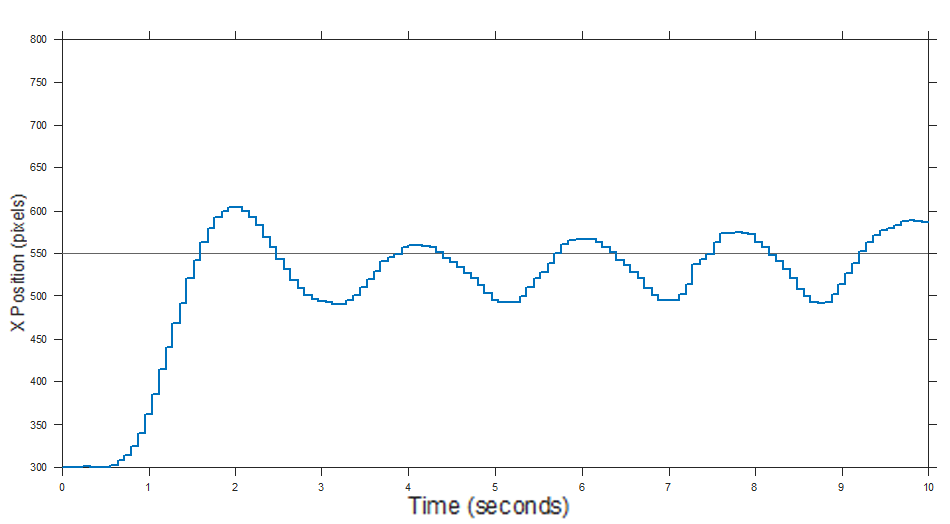
\includegraphics[width=\textwidth]{Step_response_PID1_Expiremental_x}
         \caption{PID Controller 1}
         \label{fig:y equals x}
     \end{subfigure}
     \hfill
     \begin{subfigure}[b]{0.95\textwidth}
         \centering
         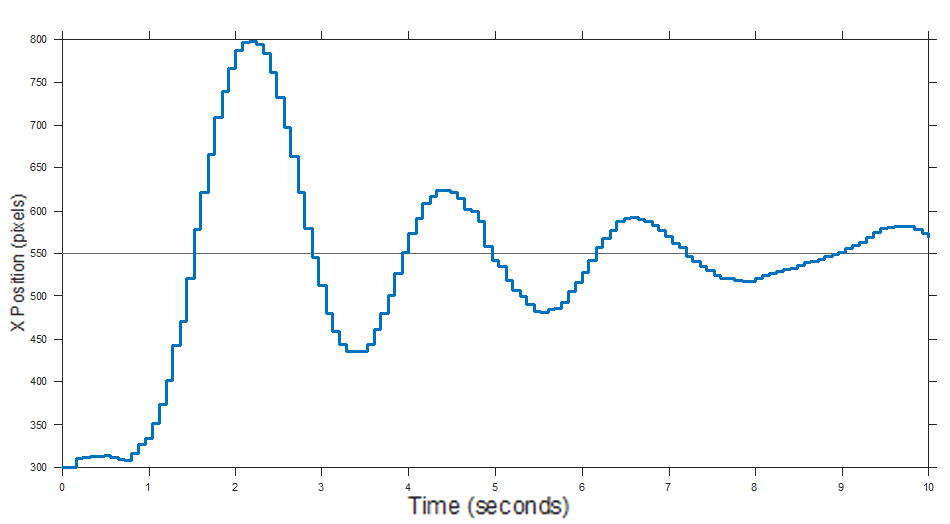
\includegraphics[width=\textwidth]{Step_response_PID2_Expiremental_x}
         \caption{PID Controller 2}
         \label{fig:three sin x}
     \end{subfigure}
     \hfill
     \begin{subfigure}[b]{0.95\textwidth}
         \centering
         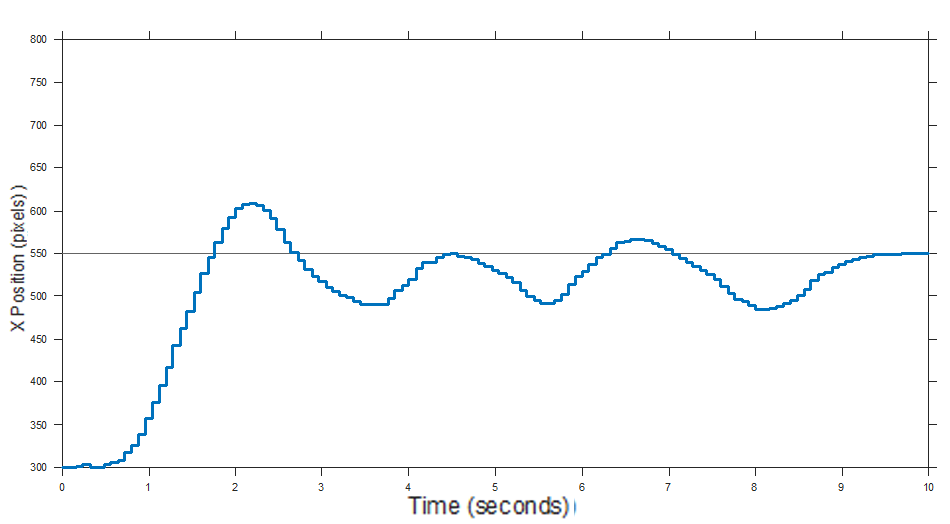
\includegraphics[width=\textwidth]{Step_response_PID3_Expiremental_x}
         \caption{PID Controller 3}
         \label{fig:five over x}
     \end{subfigure}
        \caption{Experimental Step Response and Control Output of the  BPS.}
        \label{fig:three graphs}
\end{figure}

\begin{figure}[h]
     \centering
     \begin{subfigure}[b]{1\textwidth}
         \centering
         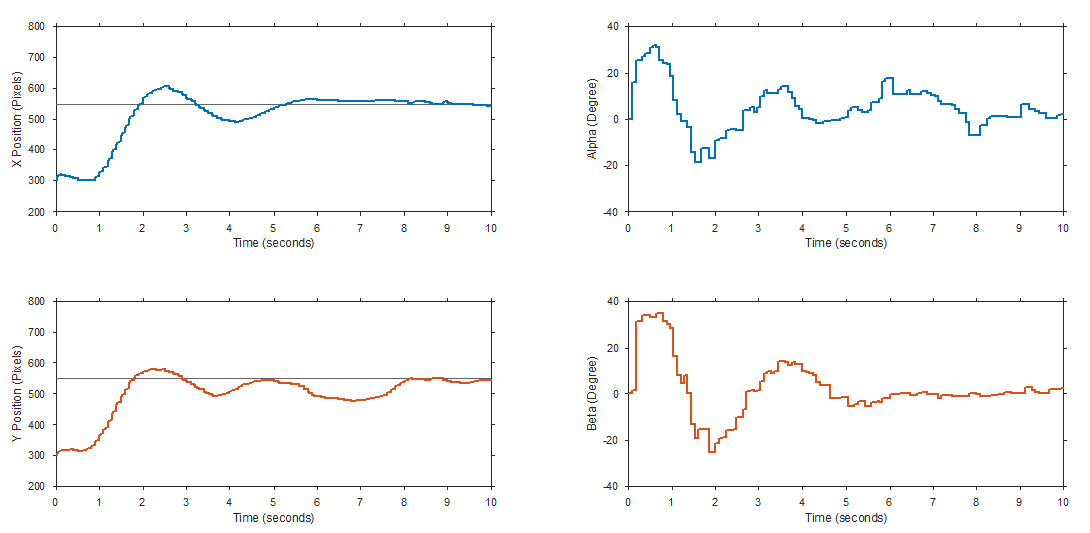
\includegraphics[width=\textwidth]{Figures/chapter05/Step_response_PID1_Expiremental.png}
         \caption{Experimental results}
         \label{fig:y equals x}
     \end{subfigure}
     \hfill
     \begin{subfigure}[b]{1\textwidth}
         \centering
         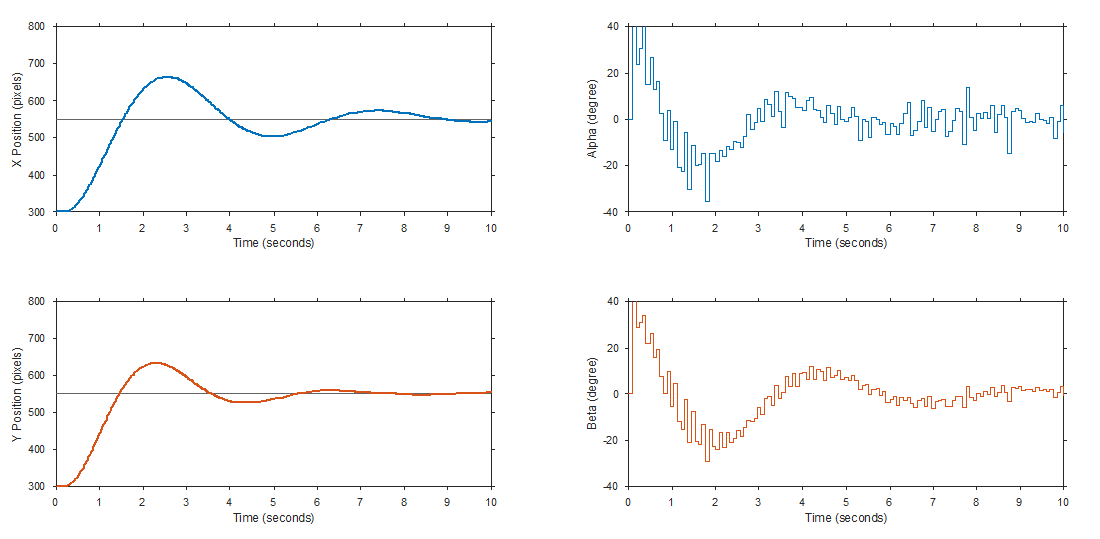
\includegraphics[width=\textwidth]{Figures/chapter05/Step_response_PID1_Simulation.png}
         \caption{Simulation result}
         \label{fig:three sin x}
     \end{subfigure}
        \caption{Step Response and Control Output of the  BPS under parameters of PID 1.}
        \label{fig:three graphs}
\end{figure}
\begin{figure}[h]
     \centering
     \begin{subfigure}[b]{1\textwidth}
         \centering
         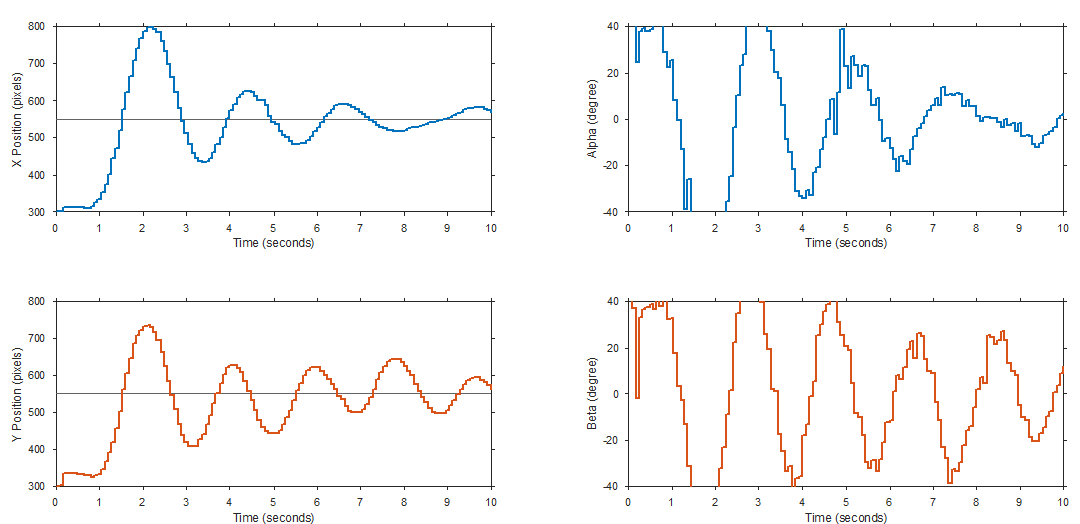
\includegraphics[width=\textwidth]{Figures/chapter05/Step_response_PID2_Expiremental.png}
         \caption{Experimental results}
         \label{fig:y equals x}
     \end{subfigure}
     \hfill
     \begin{subfigure}[b]{1\textwidth}
         \centering
         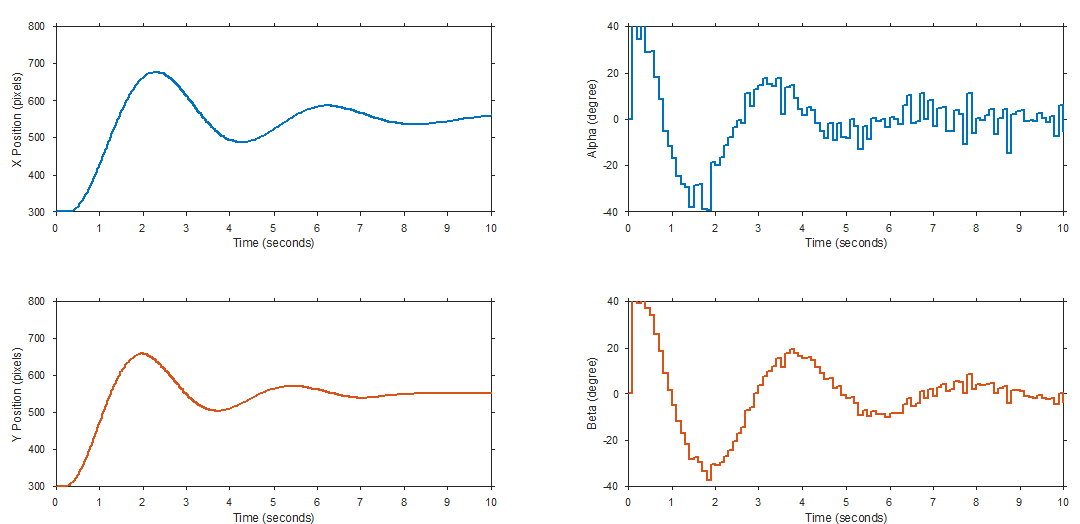
\includegraphics[width=\textwidth]{Figures/chapter05/Step_response_PID2_Simulation.png}
         \caption{Simulation result}
         \label{fig:three sin x}
     \end{subfigure}
        \caption{Step Response and Control Output of the BPS under parameters of PID 2.}
        \label{fig:three graphs}
\end{figure}
\begin{figure}[h]
     \centering
     \begin{subfigure}[b]{1\textwidth}
         \centering
         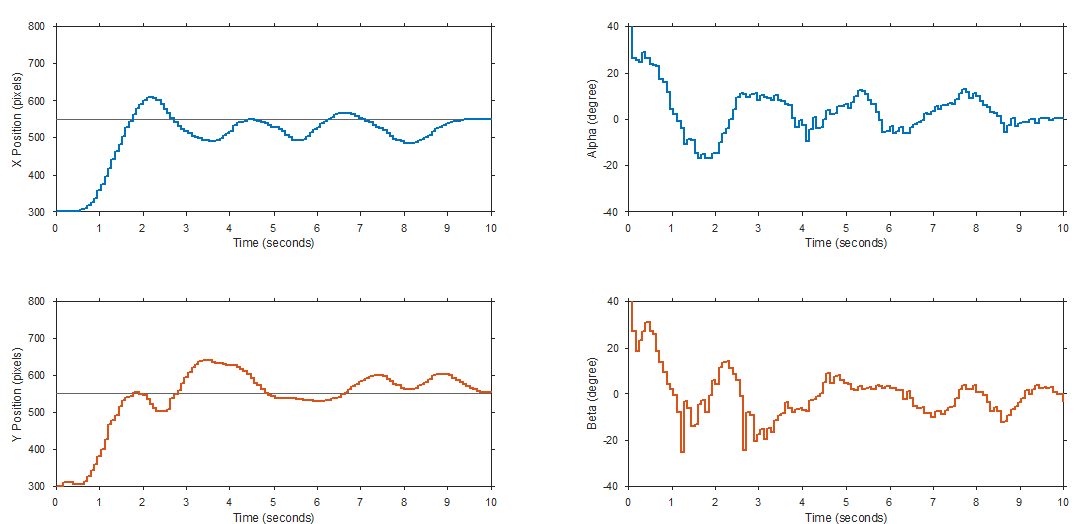
\includegraphics[width=\textwidth]{Figures/chapter05/Step_response_PID3_Expiremental.png}
         \caption{Experimental results}
         \label{fig:y equals x}
     \end{subfigure}
     \hfill
     \begin{subfigure}[b]{1\textwidth}
         \centering
         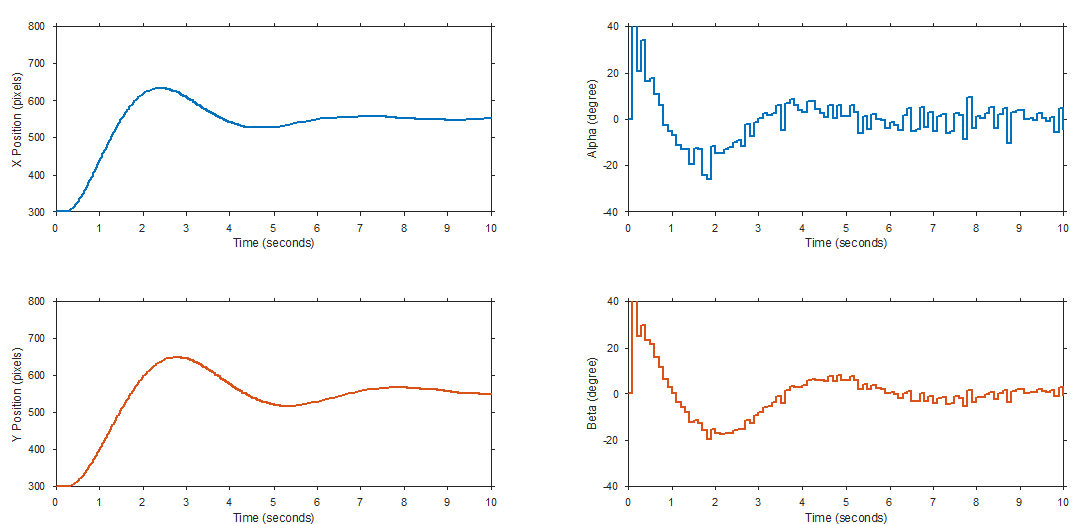
\includegraphics[width=\textwidth]{Figures/chapter05/Step_response_PID3_Simulation.png}
         \caption{Simulation result}
         \label{fig:three sin x}
     \end{subfigure}
        \caption{Step Response and Control Output of the  BPS under parameters of PID 3.}
        \label{fig:three graphs}
\end{figure}

The integral action in our controller can effectively eliminate steady-state errors, but the presence of steady-state error in the response caused by the static friction, When the ball gets close to the desired position, small tilting the plate might not be enough to overcome static friction. This can cause the ball to briefly get stuck, leading to a steady-state error that persists for a short time.
\begin{figure}[h]
     \centering
     \begin{subfigure}[b]{1\textwidth}
         \centering
         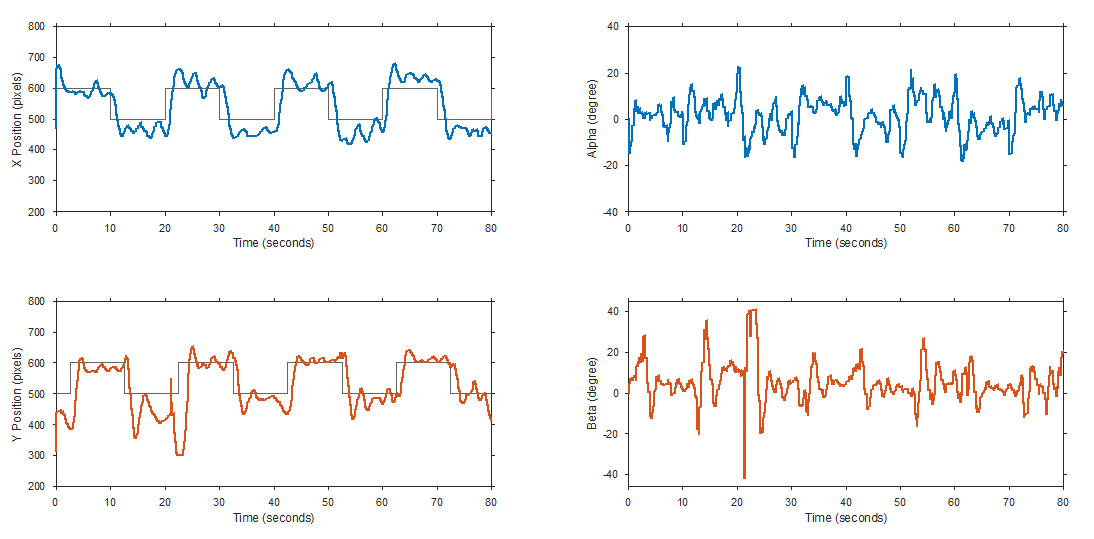
\includegraphics[width=\textwidth]{Figures/chapter05/square_tracking_PID1_Expiremental.png}
         \caption{Experimental results}
         \label{fig:y equals x}
     \end{subfigure}
     \hfill
     \begin{subfigure}[b]{1\textwidth}
         \centering
         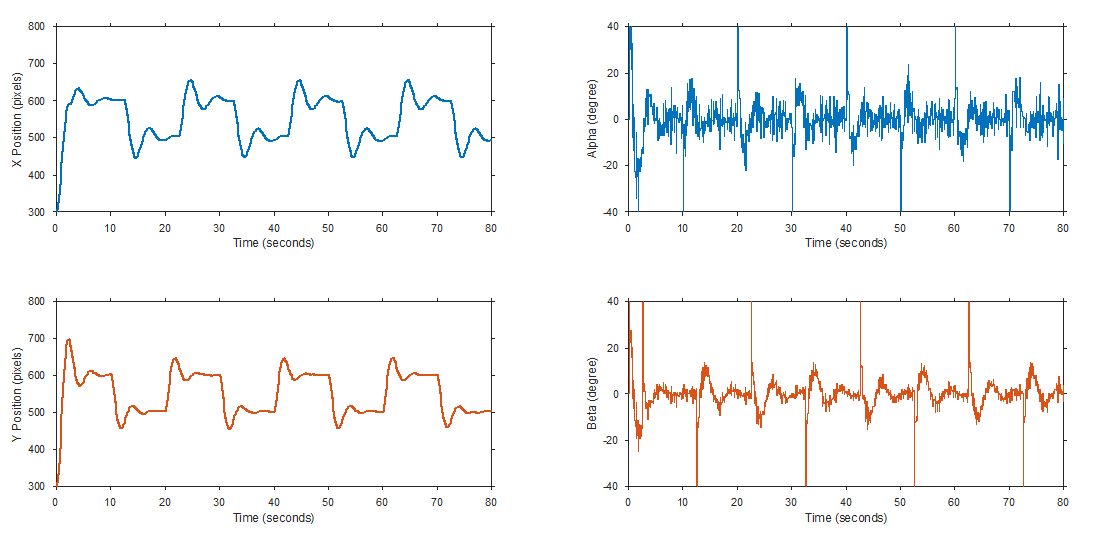
\includegraphics[width=\textwidth]{Figures/chapter05/square_tracking_PID1_simulation.png}
         \caption{Simulation result}
         \label{fig:three sin x}
     \end{subfigure}
        \caption{Square trajectory Response and Control Output of the  BPS under parameters of PID 1.}
        \label{fig:three graphs}
\end{figure}
\begin{figure}[h]
     \centering
     \begin{subfigure}[b]{1\textwidth}
         \centering
         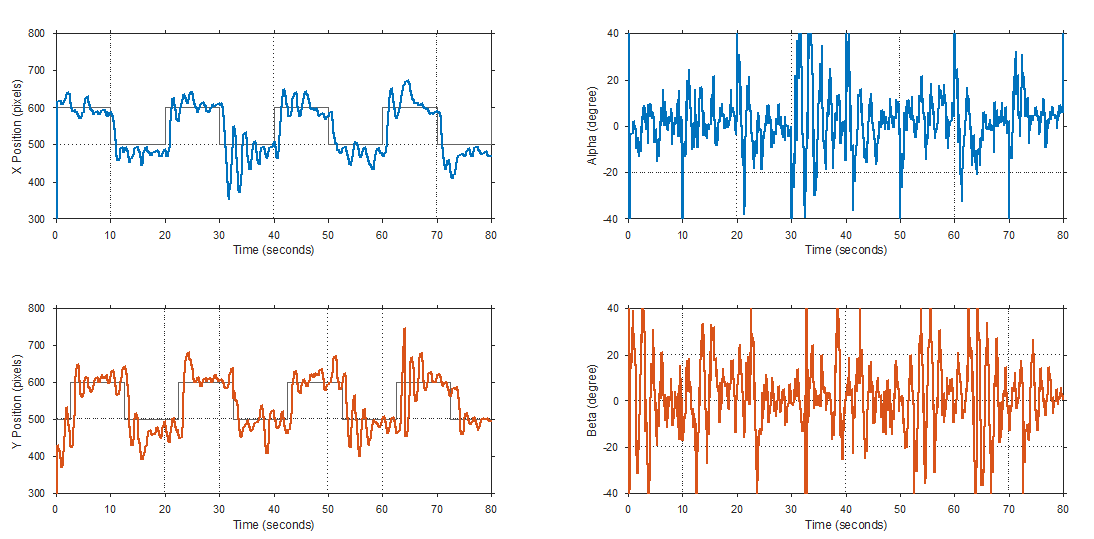
\includegraphics[width=\textwidth]{Figures/chapter05/square_tracking_PID2_Expiremental.png}
         \caption{Experimental results}
         \label{fig:y equals x}
     \end{subfigure}
     \hfill
     \begin{subfigure}[b]{1\textwidth}
         \centering
         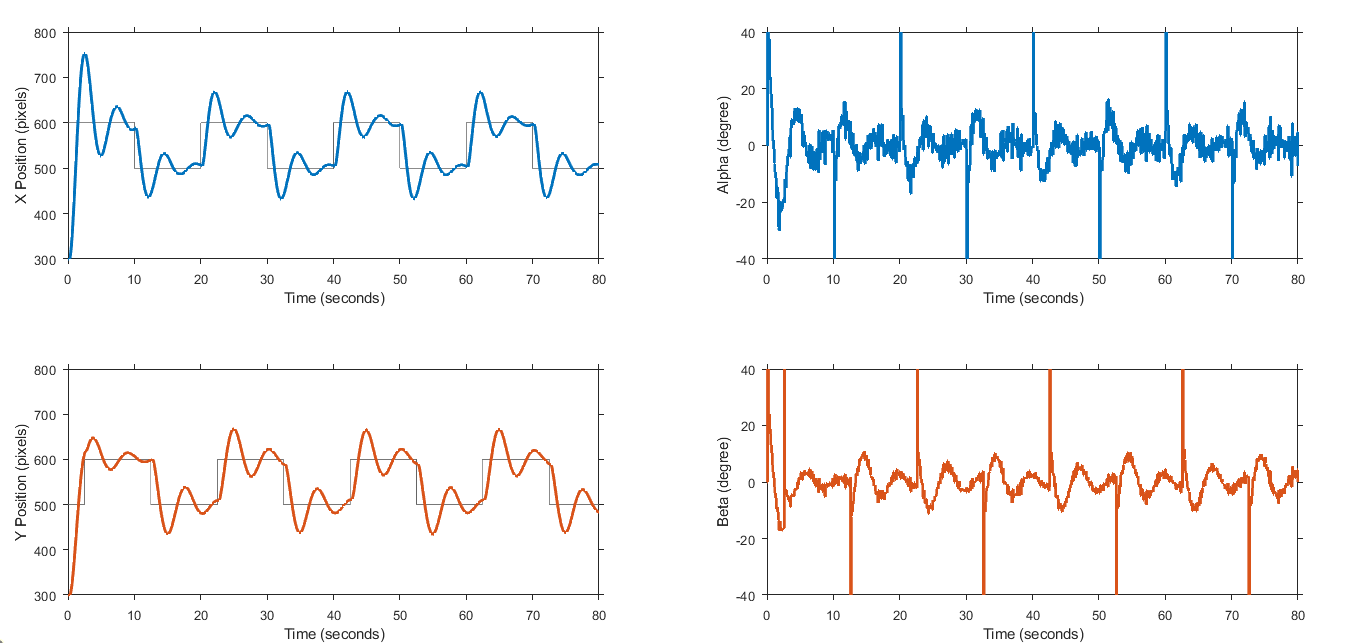
\includegraphics[width=\textwidth]{Figures/chapter05/square_tracking_PID2_simulation.png}
         \caption{Simulation result}
         \label{fig:three sin x}
     \end{subfigure}
        \caption{Square trajectory Response and Control Output of the  BPS under parameters of PID 2.}
        \label{fig:three graphs}
\end{figure}
\begin{figure}[h]
     \centering
     \begin{subfigure}[b]{1\textwidth}
         \centering
         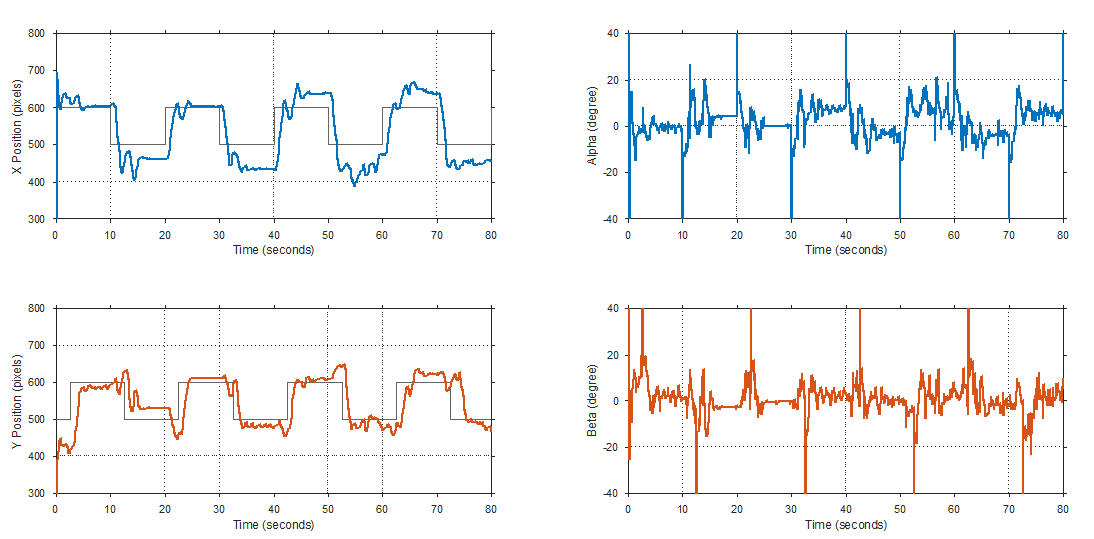
\includegraphics[width=\textwidth]{Figures/chapter05/square_tracking_PID3_Expiremental.png}
         \caption{Experimental results}
         \label{fig:y equals x}
     \end{subfigure}
     \hfill
     \begin{subfigure}[b]{1\textwidth}
         \centering
         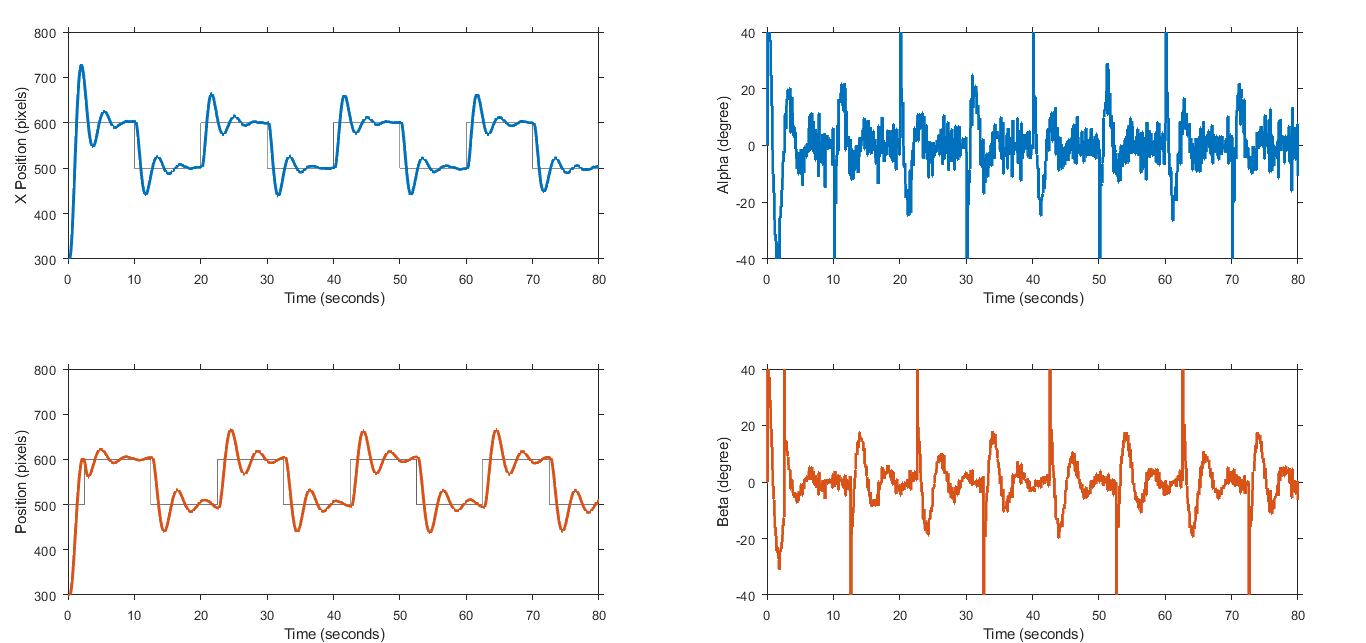
\includegraphics[width=\textwidth]{Figures/chapter05/square_tracking_PID3_simulation.png}
         \caption{Simulation result}
         \label{fig:three sin x}
     \end{subfigure}
        \caption{Square trajectory Response and Control Output of the  BPS under parameters of PID 3.}
        \label{fig:three graphs}
\end{figure}
The step response is always good to clearly see the quality of the controller’s performance, however, the plant should be able to track any reference given to it. The tracking of a square wave reference is shown in fig 5.6, 5.7, 5.8 a and b.
The issue of derivative kick is cearly shown in the control output of the figures when the angle of the controller goes extreme due to a sudden change in the input and it represent a major defect in PIDs controllers






\chapter{Conclusion and Future Work}

\section{Conclusions}
\begin{itemize}
    \item The theoretical Ball-and-Plate System (BPS) model were established and simulated, they shown promising results. The experimental implementation and testing, were less quality by the lack of adequate hardware, mainly the rods and actuators, however it still do a very good functional work 
    
    \item The BPS presents an ideal platform for control engineering students to experiment with and validate control methodologies. This is attributed to the system's cost-effectiveness and the ease with which the response can be visually observed, making it a practical and insightful tool for educational purposes.

    \item Software and programming for controlling any system is as important as theoretical control analysis, which can be an issue when approaching the challenge of building a system from an exclusive theoretical background.

    \item PID controllers remain one of the most widely employed feedback controllers. They operate by calculating an error value, representing the difference between a measured process variable and a desired set point. The controller aims to minimize this error by making adjustments to the process control inputs. However, it's important to note that PID controllers have limitations when it comes to rapidly stabilizing and mitigating the impact of disturbances  
\end{itemize}

\section{Future Work}
Numerous ways for enhancing both the plant design and controller performance are available for exploration

\begin{itemize}
    \item While the study relied on the resistive touchscreen for data acquisition, integrating a top camera could offer a more suitable solution. The touch screen, despite filtering efforts, exhibited intolerable noise and discontinuities in readings. Transitioning to a camera-based approach presents a promising alternative for precise ball position determination.

    \item  More advanced control algorithms can be explored such as Model Predictive Control (MPC), Optimal Control (LQR) or  Adaptive Control, to potentially achieve superior system stability and performance.


\end{itemize}

\begin{singlespace}
\appendix
\chapter{ِArduino code}
\begin{lstlisting}[language=C++ , caption= Arduino  full code for controlling the system by internal PID]
/*
 * Program:
 *  5_Wire_Read_servomotor_write_PID_calculate
 * Created by:
 *  Mohammed S. baayou
 * On date:
 *  2023-8-5
 * 
 * Description: This program controls a ball and plate system using a 5-wire touch panel,
 *              servo motors, and PID control to maintain the ball's position at the center.
 * Function:
 *      1. Detects ball placement on the plate using a 5-wire resistive touch panel.
 *      2. Reads ball position coordinates using a state machine approach.
 *      3. Filters sensor readings to reduce noise.
 *      4. Calibrates readings for accurate position determination.
 *      5. Implements PID control to calculate precise servo adjustments.
 *      6. Controls servo motors to tilt the plate and keep the ball balanced.
 *      7. Transitions between states to manage system behavior.
 *      8. Enters standby mode when the ball is not present to conserve energy.
 * Plan:
 *  Clean extraneous code
 */

//~~~~~~~~
//~~~~~~~~~~~~~~~~
//~~~~~~~~~~~~~~~~~~~~~~~~~~~~~~~~
//~~~~~~~~~~~~~~~~~~~~~~~~~~~~~~~~~~~~~~~~~~~~~
// LIBRARIES
//~~~~~~~~~~~~~~~~~~~~~~~~~~~~~~~~~~~~~~~~~~~~~
#include <Filters.h>
#include <Servo.h>
#include <PID_v1.h>

//~~~~~~~~~~~~~~~~~~~~~~~~~~~~~~~~~~~~~~~~~~~~~
// Variables
//~~~~~~~~~~~~~~~~~~~~~~~~~~~~~~~~~~~~~~~~~~~~~
int temp;

//~~~~~~~~~~~~~~~~~~~~~~~~~~~~~~~~
// State variables
//~~~~~~~~~~~~~~~~~~~~~~~~~~~~~~~~
int state;
unsigned long state_time;
#define STATE_STANDBY 0
#define STATE_START 1


//~~~~~~~~~~~~~~~~~~~~~~~~~~~~~~~~
// PID Variables
//~~~~~~~~~~~~~~~~~~~~~~~~~~~~~~~~
double SetpointX, InputX, OutputX;
double SetpointY, InputY, OutputY;

float xKp = 4.4;
float xKi = 0.01;
float xKd = 0.8;

//stable
//float yKp = 2.5;
//float yKi = 0.005;
//float yKd = 1.260;
float yKp = 4.2;
float yKi = 0.005;
float yKd = 0.80;

int Ts = 15;

PID myPIDX(&InputX, &OutputX, &SetpointX, xKp, xKi, xKd,
DIRECT);
PID myPIDY(&InputY, &OutputY, &SetpointY, yKp, yKi, yKd,
DIRECT);

//~~~~~~~~~~~~~~~~~~~~~~~~~~~~~~~~
// Touch panel variables
//~~~~~~~~~~~~~~~~~~~~~~~~~~~~~~~~
#define PIN_TR 2
#define PIN_TL 1
#define PIN_S  A1
#define PIN_SD 5
#define PIN_BL 4
#define PIN_BR 3
#define SETTLE_TIME 5


float x_pos, y_pos;
float pre_pos = 810;
unsigned long panel_time;
int standByValue = 0 ;
unsigned int noTouchCount = 0;

//Caliboration
float Caliboration_Xscale = 800/34;
float Caliboration_Yscale = 800/34;
float Xoffset = 550;
float Yoffset = 550;
//~~~~~~~~~~~~~~~~~~~~~~~~~~~~~~~~
// low pass filters variables
//~~~~~~~~~~~~~~~~~~~~~~~~~~~~~~~~
 float filterFrequencyX= 5;
 float filterFrequencyY= 4;
 int InputXfiltered, InputYfiltered;

 // Initializing a one pole (RC) lowpass filter
 FilterOnePole lowpassFilterX( LOWPASS, filterFrequencyX );
 FilterOnePole lowpassFilterY( LOWPASS, filterFrequencyY );


//~~~~~~~~~~~~~~~~~~~~~~~~~~~~~~~~
// Servo.h Instllation 
//~~~~~~~~~~~~~~~~~~~~~~~~~~~~~~~~
Servo myservoX;
Servo myservoY;

double angleX;
double angleY;

double flatAngleX = 72;
double flatAngleY = 75;

int stableCount = 0;

#define PIN_X 9
#define PIN_Y 8

void setup()
{ 
  //~~~~~~~~~~~~~~~~~~~~~~~~~~~~~~~~
  // Establish pin modes
  //~~~~~~~~~~~~~~~~~~~~~~~~~~~~~~~~
  // Touch panel
  pinMode(PIN_TR, OUTPUT);
  pinMode(PIN_TL, OUTPUT);
  pinMode(PIN_BL, OUTPUT);
  pinMode(PIN_BR, OUTPUT);
  digitalWrite(PIN_TR, LOW);
  digitalWrite(PIN_TL, LOW);
  digitalWrite(PIN_BL, LOW);
  digitalWrite(PIN_BR, LOW);
  pinMode(PIN_S, INPUT);

  //~~~~~~~~~~~~~~~~~~~~~~~~~~~~~~~~
  // Initialize variables
  //~~~~~~~~~~~~~~~~~~~~~~~~~~~~~~~~
  // State Machine
  state = 0;

  //~~~~~~~~~~~~~~~~~~~~~~~~~~~~~~~~
  // Servo Motors
  //~~~~~~~~~~~~~~~~~~~~~~~~~~~~~~~~
  // Attach Servo motors to pins
  myservoX.attach(PIN_X);
  myservoY.attach(PIN_Y);

  OutputX = flatAngleX;
  OutputY = flatAngleY;

  myservoX.write(OutputX);
  myservoY.write(OutputY);

// Setting starting parameters for PID
  myPIDX.SetMode(AUTOMATIC);
  myPIDY.SetMode(AUTOMATIC);
  InputX = 0;
  InputY = 0;

  SetpointX = 0.00;
  SetpointY = 0.00;

  // Setting limiting parameters for servo motors
  myPIDX.SetOutputLimits(flatAngleX-85, flatAngleX+85);
  myPIDY.SetOutputLimits(flatAngleY-85, flatAngleY+85);

  myPIDX.SetSampleTime(Ts);
  myPIDY.SetSampleTime(Ts);

  angleX = flatAngleX;
  angleY = flatAngleY;

  



  //~~~~~~~~~~~~~~~~~~~~~~~~~~~~~~~~
  // Begin Serial Communication
  //~~~~~~~~~~~~~~~~~~~~~~~~~~~~~~~~
  Serial.begin(9600);
}

void loop()
{
  switch(state)
  {
    case 0: //standby mode
      pinMode(PIN_TR, OUTPUT);
      pinMode(PIN_TL, OUTPUT);
      pinMode(PIN_BL, OUTPUT);
      pinMode(PIN_BR, OUTPUT);
      digitalWrite(PIN_TR, LOW);
      digitalWrite(PIN_TL, LOW);
      digitalWrite(PIN_BL, LOW);
      digitalWrite(PIN_BR, LOW);

      pinMode(PIN_S, INPUT_PULLUP );
      delay(10);

      standByValue = analogRead(PIN_S);
      //Serial.println(noTouchCount);
      //Serial.print("\t");
      if(standByValue < 800){
        state = 1;
        myservoX.attach(PIN_X);
        myservoY.attach(PIN_Y);
        noTouchCount = 0; 
      }
      else{
        noTouchCount++;

          myservoX.write(OutputX); 
          myservoY.write(OutputY); 
        if(noTouchCount > 100) //if there is no ball on plate longer
        {

          OutputX=flatAngleX; //make plate flat
          OutputY=flatAngleY;
          myservoX.write(OutputX); 
          myservoY.write(OutputY); 
          delay(1000);   
          myservoX.detach(); //detach servos
          myservoY.detach();   
          break;  
        }

      }
      //state=1;
      break;


    case 1: // Set up X read mode
      //~~~~~~~~~~~~~~~~
      // Set up X read
      //~~~~~~~~~~~~~~~~
      // Set TR and BR high
      digitalWrite(PIN_TR, LOW);
      digitalWrite(PIN_BR, LOW);
      // Set TL and BL low
      digitalWrite(PIN_TL, HIGH);
      digitalWrite(PIN_BL, HIGH);

      //~~~~~~~~~~~~~~~~
      // Move to next state
      //~~~~~~~~~~~~~~~~
      // Record the time
      panel_time = millis();
      // Switch to waiting for the panel to settle
      state = 2;
      break;
    
    case 2: // Reading X position mode
      // How long has it been since the panel changed configuration?
      temp = millis() - panel_time;
      // Has it been long enough?
      if (temp >= SETTLE_TIME)
      { // If it has...
        pre_pos = x_pos; 
        x_pos = analogRead(PIN_S);
        //filtering no touch spikes
        if (x_pos > 900){
          x_pos = pre_pos;
        }
        // Switch to the Read X state
        state = 3;
      } // Otherwise, do nothing.
      break;

    case 3: // Set up Y read mode
      //~~~~~~~~~~~~~~~~
      // Set up Y read
      //~~~~~~~~~~~~~~~~
      // Set TR and TL high
      digitalWrite(PIN_TR, HIGH);
      digitalWrite(PIN_TL, HIGH);
      // Set BL and BR low
      digitalWrite(PIN_BL, LOW);
      digitalWrite(PIN_BR, LOW);

      //~~~~~~~~~~~~~~~~
      // Move to next state
      //~~~~~~~~~~~~~~~~
      // Record the time
      panel_time = millis();
      // Switch to waiting for the panel to settle
      state = 4;

      break;
      
    case 4: // Reading Y position mode
      // How long has it been since the panel changed configuration?
      temp = millis() - panel_time;
      
      // Has it been long enough?
      if (temp >= SETTLE_TIME)
      { // If it has...
        // Read the sensor voltage (Y position)
        pre_pos = y_pos; 
        y_pos = analogRead(PIN_S);
        if (y_pos > 800){
          y_pos = pre_pos;
        }
          state = 5;
      } // Otherwise, do nothing.
      break;
    

    case 5: // testing & filtering coordinates mode
      //----------------------------------
      //Serial.print(x_pos);
      //Serial.print("\t");
      //Serial.print(y_pos);
      //Serial.print("\t");
      
      // Filtering touchpanel signal
      x_pos = lowpassFilterX.input(x_pos);
      y_pos = lowpassFilterY.input(y_pos);

      // Write the coordinates to Serial for debuging
      //Serial.print("filtered coordinates  ");
      //Serial.print(x_pos);
      //Serial.print("\t");
      //Serial.print(y_pos);
      //Serial.print("\n");

      state = 6;
      //--------------------------------
      break;

    case 6: // Caliboration & checking if the ball in the center
      InputX = (x_pos - Xoffset) / Caliboration_Xscale;
      InputY = (y_pos - Yoffset) / Caliboration_Yscale;
      //Serial.print("Caliborated position  ");
      Serial.print("\t");
      Serial.print(InputX);
      Serial.print("\t");
      Serial.print(InputY);
      //Serial.print("\n");

      if(InputX <= SetpointX + 0.85 && InputX >= SetpointX - 0.85 && InputY <= SetpointY + 1.25 && InputY >= SetpointY - 1.25 ){
        stableCount++;
      }
      else{
        stableCount =- 2;
      }
        
      if(stableCount > 150){
        myservoX.write(flatAngleX); 
        myservoY.write(flatAngleY);
        //delay(1000);
        state = 8;
        break;
      }
      state = 7;
      break;

    case 7: // setting PID outputs


      myPIDX.Compute();  //action control X compute
      myPIDY.Compute();  //   action control  Y compute  

      myservoX.write(OutputX); 
      myservoY.write(OutputY);

      //Serial.print("servos angle  ");
      //Serial.print("\t");
      //Serial.print(OutputX);
      //Serial.print("\t");
      //Serial.print(OutputY);
      Serial.println("\n");

      state = 8;
      break;


    case 8: // Turn off the panel
      // Turn off the panel
      digitalWrite(PIN_TR, LOW);
      digitalWrite(PIN_TL, LOW);
      digitalWrite(PIN_BL, LOW);
      digitalWrite(PIN_BR, LOW);

      // Switch to button debounce state
      state = 9;
      break;


    case 9: // End state
      
      // Send message through Serial
      //Serial.println("Panel read finished");
      delay(20);

      // Switch to the waiting state
      state = 0;
      break;
      
    default: // Error
      Serial.println("Something has gone terribly wrong.");
      break;
    }
  }
\end{lstlisting}

\begin{lstlisting}[language=C++ , caption= Arduino full code for controlling the system by a simulink controller]
/*
 * Program:
 *  5_Wire_Read_servomotor_write_PID_calculate
 * Created by:
 *  Mohammed S. baayou
 * On date:
 *  2023-8-5
 * 
 * Description: This program controls a ball and plate system using a 5-wire touch panel,
 *              servo motors, and PID control to maintain the ball's position at the center.
 * Function:
 *      1. Detects ball placement on the plate using a 5-wire resistive touch panel.
 *      2. Reads ball position coordinates using a state machine approach.
 *      3. Filters sensor readings to reduce noise.
 *      4. Calibrates readings for accurate position determination.
 *      5. Implements PID control to calculate precise servo adjustments.
 *      6. Controls servo motors to tilt the plate and keep the ball balanced.
 *      7. Transitions between states to manage system behavior.
 *      8. Enters standby mode when the ball is not present to conserve energy.
 * Plan:
 *  Clean comments and extraneous code
 */

//~~~~~~~~
//~~~~~~~~~~~~~~~~
//~~~~~~~~~~~~~~~~~~~~~~~~~~~~~~~~
//~~~~~~~~~~~~~~~~~~~~~~~~~~~~~~~~~~~~~~~~~~~~~~
// LIBRARIES
//~~~~~~~~~~~~~~~~~~~~~~~~~~~~~~~~~~~~~~~~~~~~~~
#include <Servo.h>
//~~~~~~~~~~~~~~~~~~~~~~~~~~~~~~~~~~~~~~~~~~~~~~
// Variables
//~~~~~~~~~~~~~~~~~~~~~~~~~~~~~~~~~~~~~~~~~~~~~~
int temp;

//~~~~~~~~~~~~~~~~~~~~~~~~~~~~~~~~
// State variables
//~~~~~~~~~~~~~~~~~~~~~~~~~~~~~~~~
int state;
unsigned long state_time;
#define STATE_STANDBY 0
#define STATE_START 1


int Ts = 15;



//~~~~~~~~~~~~~~~~~~~~~~~~~~~~~~~~
// Touch panel variables
//~~~~~~~~~~~~~~~~~~~~~~~~~~~~~~~~
#define PIN_TR 3
#define PIN_TL 2
#define PIN_S  A1
#define PIN_SD 6
#define PIN_BL 5
#define PIN_BR 4
#define SETTLE_TIME 5


float x_pos, y_pos;
float pre_pos = 810;
unsigned long panel_time;
int standByValue = 0 ;
unsigned int noTouchCount = 0;
char header;

//~~~~~~~~~~~~~~~~~~~~~~~~~~~~~~~~
//Caliboration
//~~~~~~~~~~~~~~~~~~~~~~~~~~~~~~~~
float Caliboration_Xscale = 800/34;
float Caliboration_Yscale = 800/28;
float Xoffset = 550;
float Yoffset = 550;

//~~~~~~~~~~~~~~~~~~~~~~~~~~~~~~~~
// Servo.h Instllation 
//~~~~~~~~~~~~~~~~~~~~~~~~~~~~~~~~
Servo myservoX;
Servo myservoY;
double angleX;
double angleY;
double flatAngleX = 72;
double flatAngleY = 75;
//int outputX = flatAngleX;
//int outputY = flatAngleY;
#define PIN_X 9
#define PIN_Y 8

int stableCount = 0;

typedef union{
  float number;
  uint8_t bytes[4];
} FLOATUNION_t;

FLOATUNION_t sendX1;
FLOATUNION_t sendY2;

FLOATUNION_t xValue;
FLOATUNION_t yValue;

void setup()
{ 
  //~~~~~~~~~~~~~~~~~~~~~~~~~~~~~~~~
  // Establish pin modes
  //~~~~~~~~~~~~~~~~~~~~~~~~~~~~~~~~
  // Touch panel
  pinMode(PIN_TR, OUTPUT);
  pinMode(PIN_TL, OUTPUT);
  pinMode(PIN_BL, OUTPUT);
  pinMode(PIN_BR, OUTPUT);
  digitalWrite(PIN_TR, LOW);
  digitalWrite(PIN_TL, LOW);
  digitalWrite(PIN_BL, LOW);
  digitalWrite(PIN_BR, LOW);
  pinMode(PIN_S, INPUT);

  //~~~~~~~~~~~~~~~~~~~~~~~~~~~~~~~~
  // Initialize variables
  //~~~~~~~~~~~~~~~~~~~~~~~~~~~~~~~~
  // State Machine
  state = 0;


//~~~~~~~~~~~~~~~~~~~~~~~~~~~~~~~~
  // Servo Motors
  //~~~~~~~~~~~~~~~~~~~~~~~~~~~~~~~~
  // Attach Servo motors to pins
  myservoX.attach(PIN_X);
  myservoY.attach(PIN_Y);

  xValue.number = flatAngleX;
  yValue.number = flatAngleY;
  angleX = flatAngleX;
  angleY = flatAngleY;

  myservoX.write(flatAngleX);
  myservoY.write(flatAngleY);



  //~~~~~~~~~~~~~~~~~~~~~~~~~~~~~~~~
  // Begin Serial Communication
  //~~~~~~~~~~~~~~~~~~~~~~~~~~~~~~~~
  Serial.begin(9600);
}

void loop()
{
  switch(state)
  {
    case 0: //standby mode
      pinMode(PIN_TR, OUTPUT);
      pinMode(PIN_TL, OUTPUT);
      pinMode(PIN_BL, OUTPUT);
      pinMode(PIN_BR, OUTPUT);
      digitalWrite(PIN_TR, LOW);
      digitalWrite(PIN_TL, LOW);
      digitalWrite(PIN_BL, LOW);
      digitalWrite(PIN_BR, LOW);

      pinMode(PIN_S, INPUT_PULLUP );
      delay(10);

      standByValue = analogRead(PIN_S);

      if(standByValue < 800){
        state = 1;
        myservoX.attach(PIN_X);
        myservoY.attach(PIN_Y);
        noTouchCount = 0; 
      }
      else{
        noTouchCount++;
        myservoX.write(angleX); 
        myservoY.write(angleY); 
        if(noTouchCount > 100) //if there is no ball on plate longer
        {
          myservoX.write(flatAngleX); 
          myservoY.write(flatAngleY); 
          delay(1000);   
          myservoX.detach(); //detach servos
          myservoY.detach();   
          break;          }

      }
      break;


    case 1: // Set up X read mode
      //~~~~~~~~~~~~~~~~
      // Set up X read
      //~~~~~~~~~~~~~~~~
      // Set TR and BR high
      digitalWrite(PIN_TR, LOW);
      digitalWrite(PIN_BR, LOW);
      // Set TL and BL low
      digitalWrite(PIN_TL, HIGH);
      digitalWrite(PIN_BL, HIGH);

      //~~~~~~~~~~~~~~~~
      // Move to next state
      //~~~~~~~~~~~~~~~~
      // Record the time
      panel_time = millis();
      // Switch to waiting for the panel to settle
      state = 2;
      break;
    
    case 2: // Reading X position mode
      // How long has it been since the panel changed configuration?
      temp = millis() - panel_time;
      // Has it been long enough?
      if (temp >= SETTLE_TIME)
      { // If it has...
        pre_pos = x_pos; 
        x_pos = analogRead(PIN_S);
        //filtering no touch spikes
        if (x_pos > 900){
          x_pos = pre_pos;
        }
        // Switch to the Read X state
        state = 3;
      } // Otherwise, do nothing.
      break;

    case 3: // Set up Y read mode
      //~~~~~~~~~~~~~~~~
      // Set up Y read
      //~~~~~~~~~~~~~~~~
      // Set TR and TL high
      digitalWrite(PIN_TR, HIGH);
      digitalWrite(PIN_TL, HIGH);
      // Set BL and BR low
      digitalWrite(PIN_BL, LOW);
      digitalWrite(PIN_BR, LOW);

      //~~~~~~~~~~~~~~~~
      // Move to next state
      //~~~~~~~~~~~~~~~~
      // Record the time
      panel_time = millis();
      // Switch to waiting for the panel to settle
      state = 4;

      break;
      
    case 4: // Reading Y position mode
      // How long has it been since the panel changed configuration?
      temp = millis() - panel_time;
      
      // Has it been long enough?
      if (temp >= SETTLE_TIME)
      { // If it has...
        // Read the sensor voltage (Y position)
        pre_pos = y_pos; 
        y_pos = analogRead(PIN_S);
        if (y_pos > 800){
          y_pos = pre_pos;
        }
          state = 5;
      } // Otherwise, do nothing.
      break;
    

    case 5: // packeting & sending coordinates via serial communication
    
      //----------------------------------
      //x_pos = (x_pos - Xoffset) / Caliboration_Xscale;
      //y_pos = (y_pos - Yoffset) / Caliboration_Yscale;
      //----------------------------------
      sendX1.number = x_pos;
      sendY2.number = y_pos;
      if( x_pos > 0 && y_pos > 0){

        Serial.print("A");

        for (int i=0; i<4; i++){
          Serial.write(sendX1.bytes[i]); 
        }

        for (int i=0; i<4; i++){
          Serial.write(sendY2.bytes[i]); 
        }

        Serial.print("\n");
        delay(50);

        state = 6;
        //--------------------------------
        break;
      }
      state = 0;
      break;


    case 6: // recieving servo angles

      if (Serial.available() >= 8) {
        xValue.number = getFloat();
        angleX = xValue.number;
        yValue.number = getFloat();
        angleY = yValue.number;
      }

      if(isnan(angleX) || isnan(angleY) || angleY == 0 || angleX == 0){
        //Serial.flush();
        state = 7;
        break;
      }

      myservoX.write(angleX); 
      myservoY.write(angleY);

      state = 7;
      break;
    
    
    case 7: // Turn off the panel
      // Turn off the panel
      digitalWrite(PIN_TR, LOW);
      digitalWrite(PIN_TL, LOW);
      digitalWrite(PIN_BL, LOW);
      digitalWrite(PIN_BR, LOW);

      // Switch to button debounce state
      state = 0;
      break;
      
    default: // Error
      Serial.println("Something has gone terribly wrong.");
      break;
    }
  }

float getFloat(){
    int cont = 0;
    FLOATUNION_t f;
    while (cont < 4 ){
        f.bytes[cont] = Serial.read() ;
        cont = cont +1;
    } 
    return f.number;
}
\end{lstlisting}


\chapter{Simulink Block diagram}
\begin{figure}[h]
    \centering
    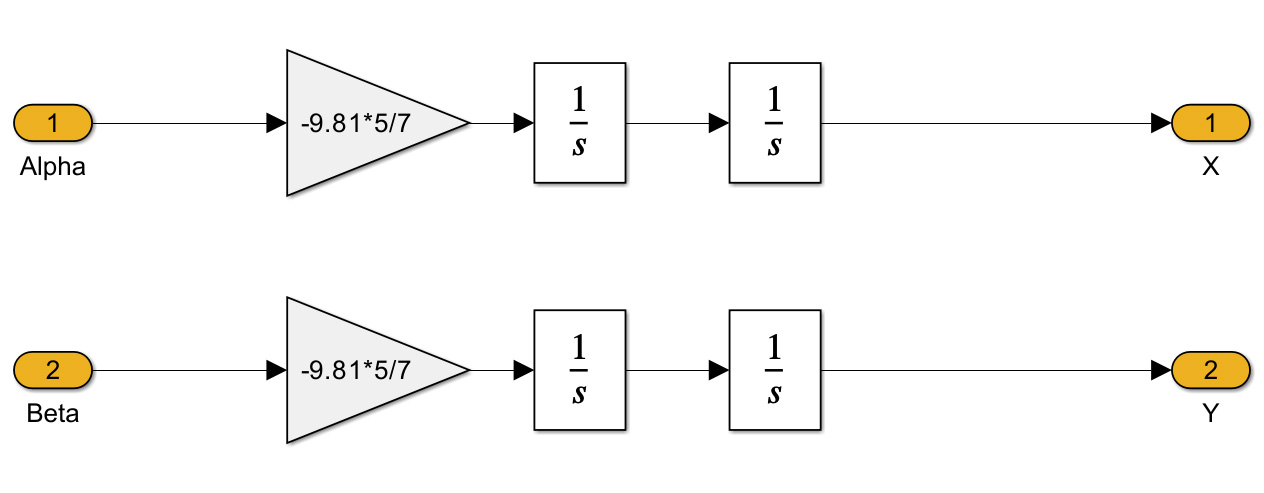
\includegraphics[width=1\linewidth]{Figures/chapter03/Linear_BPS_Simulink_Model_inTransferFunction.jpg}
    \caption{Linear simulation model of the Ball and Plate System in a transfer function form}

\end{figure}
\begin{figure}
    \centering
    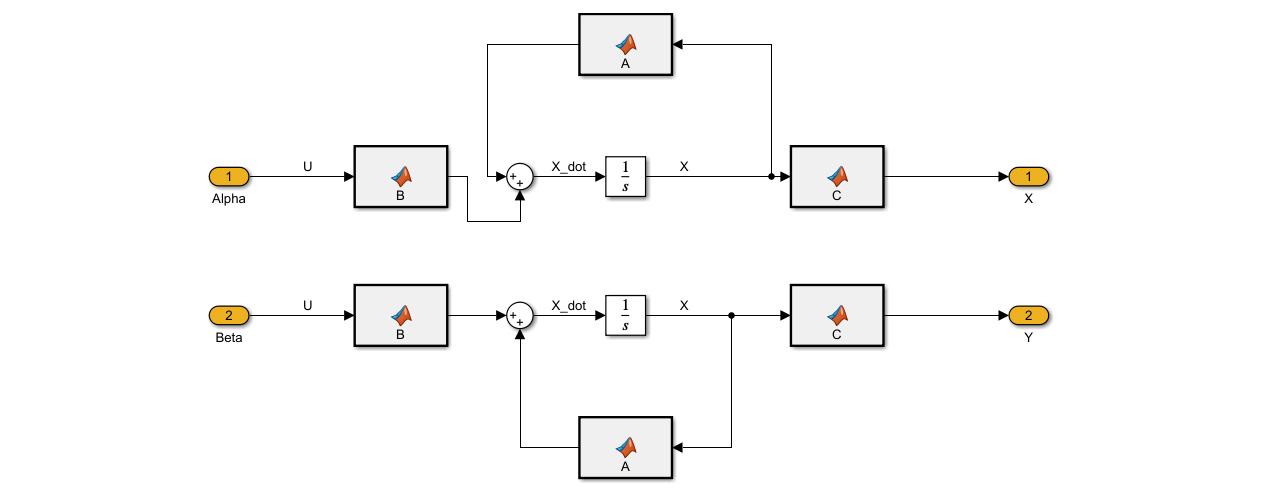
\includegraphics[width=1\linewidth]{Figures/chapter03/Linear_BPS_Simulink_Model_inStateSpace.jpg}
    \caption{Linear simulation model of the Ball and Plate System in state-space form}
\end{figure}

\begin{sidewaysfigure}
\centering
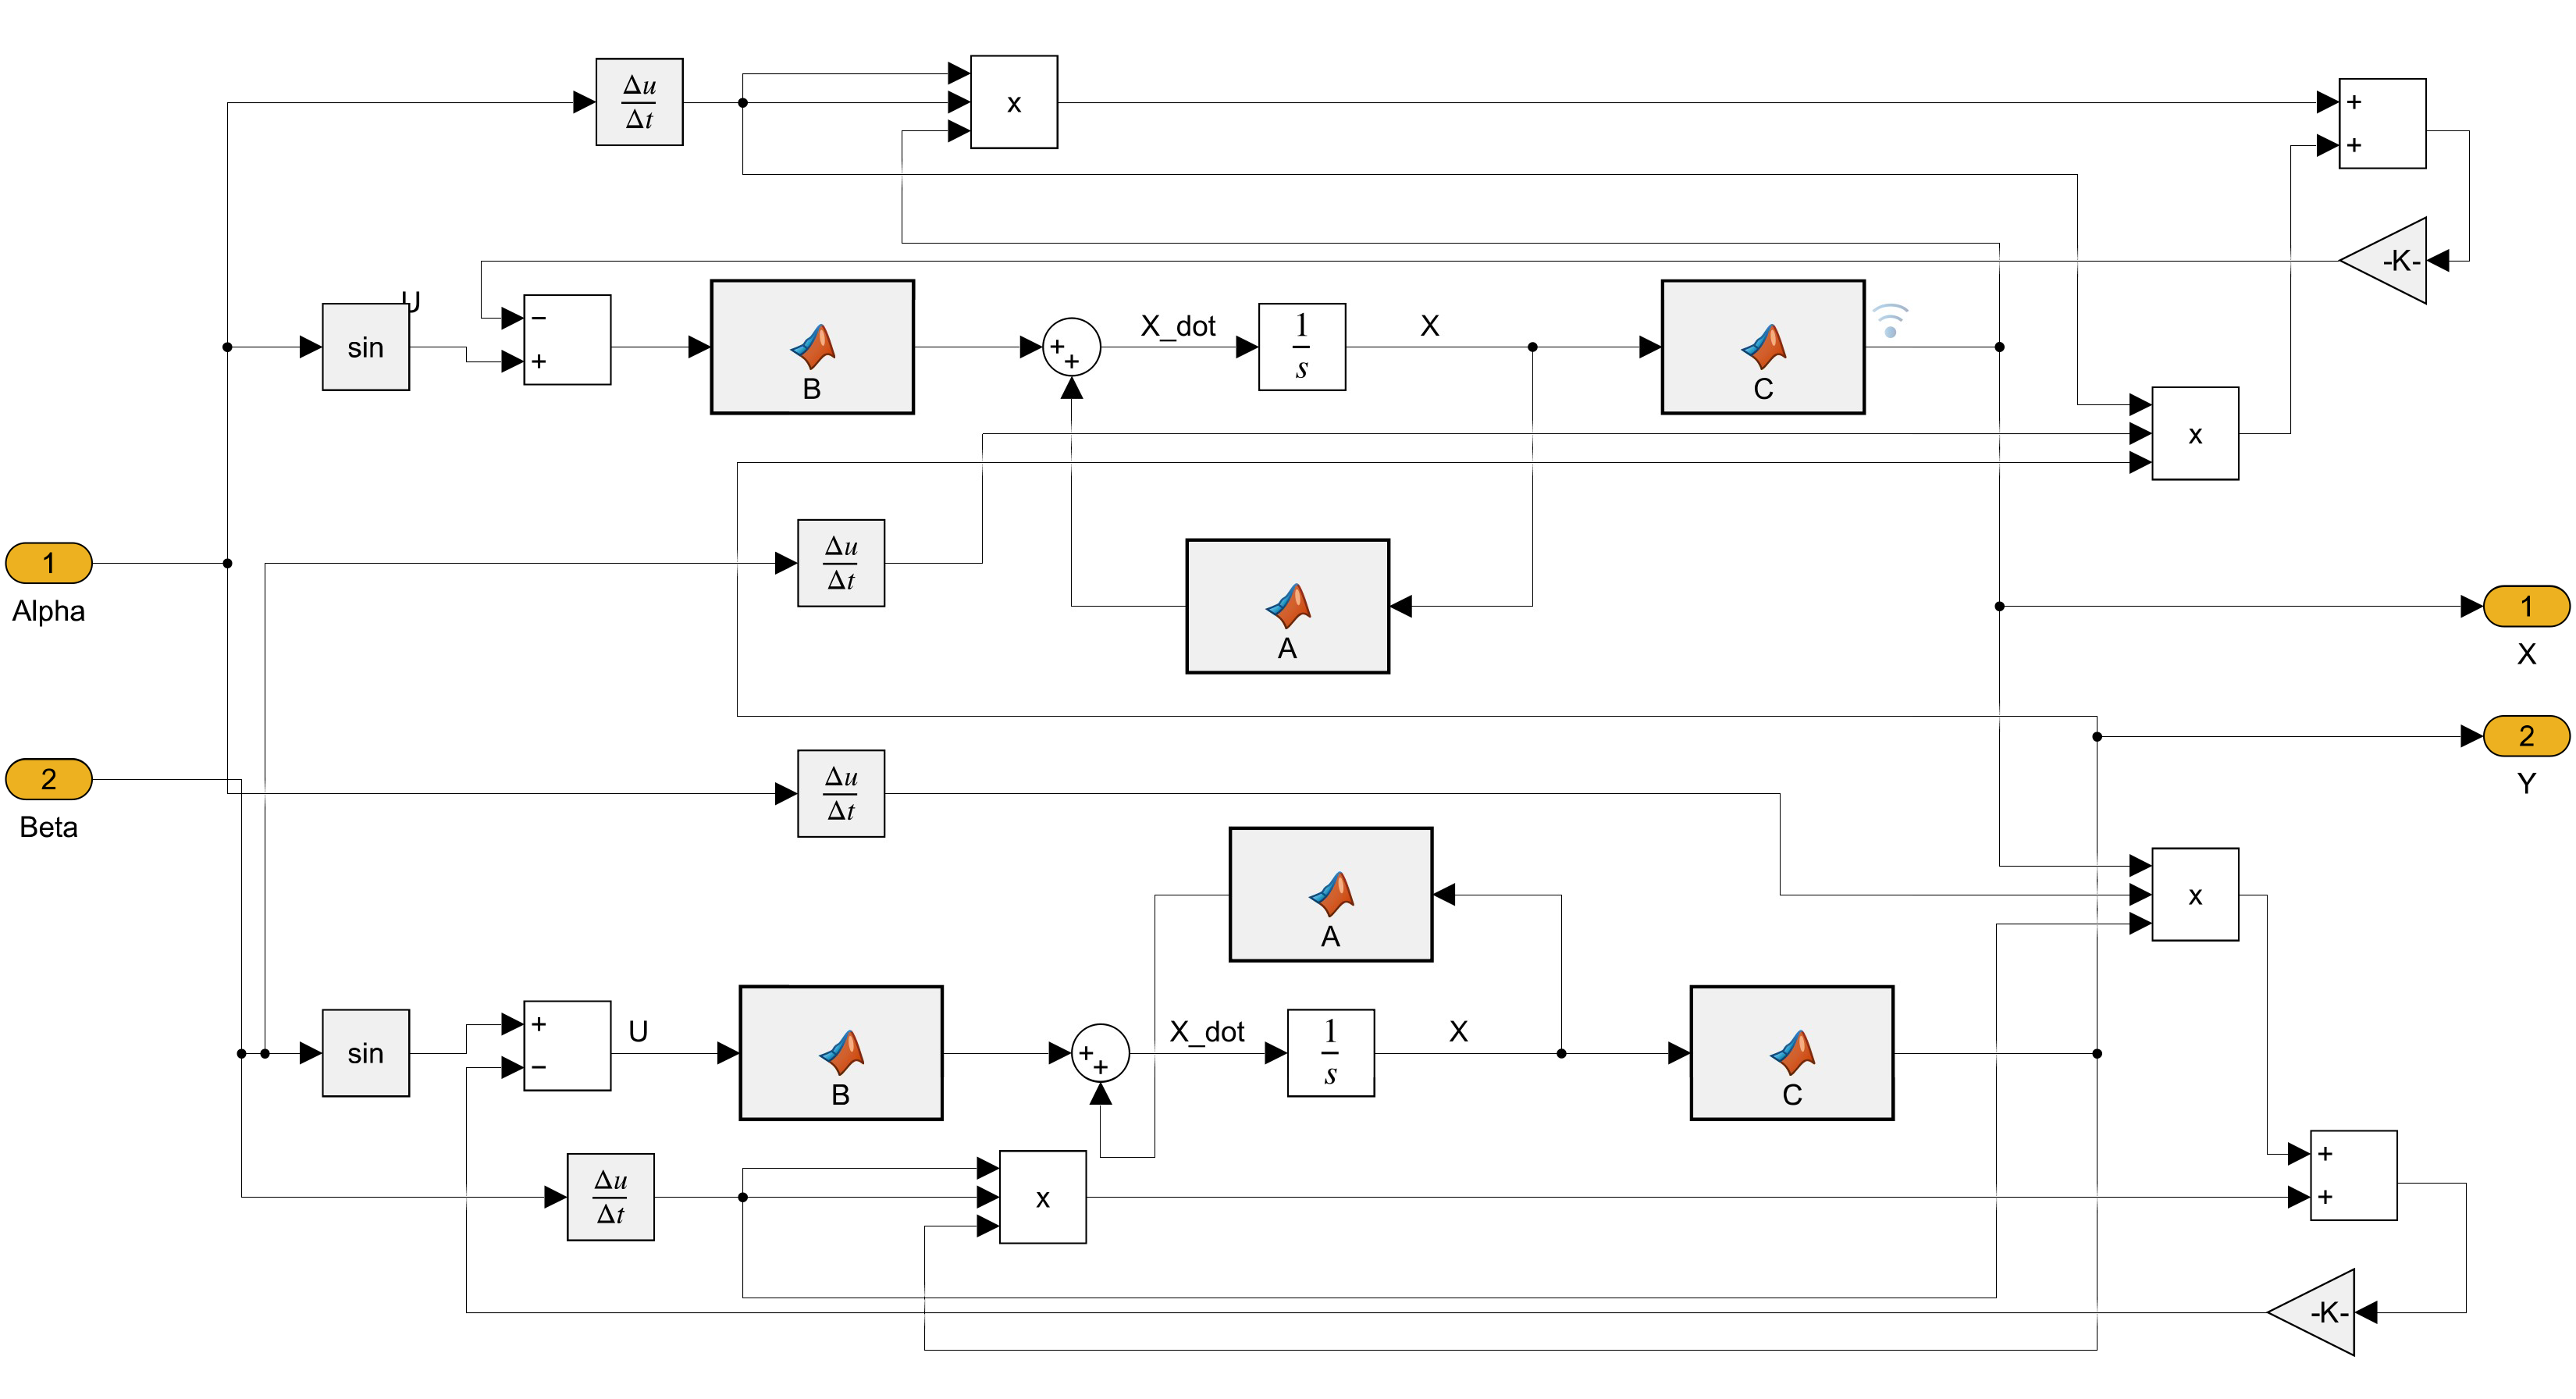
\includegraphics[width=0.95\textheight]{Figures/chapter03/nonlinear.png}
\caption{Approximated representation of the non-linear BPS dynamics in a Simulink model}
\label{fig:IMs matrix correlation}
\end{sidewaysfigure}

\begin{sidewaysfigure}
\centering
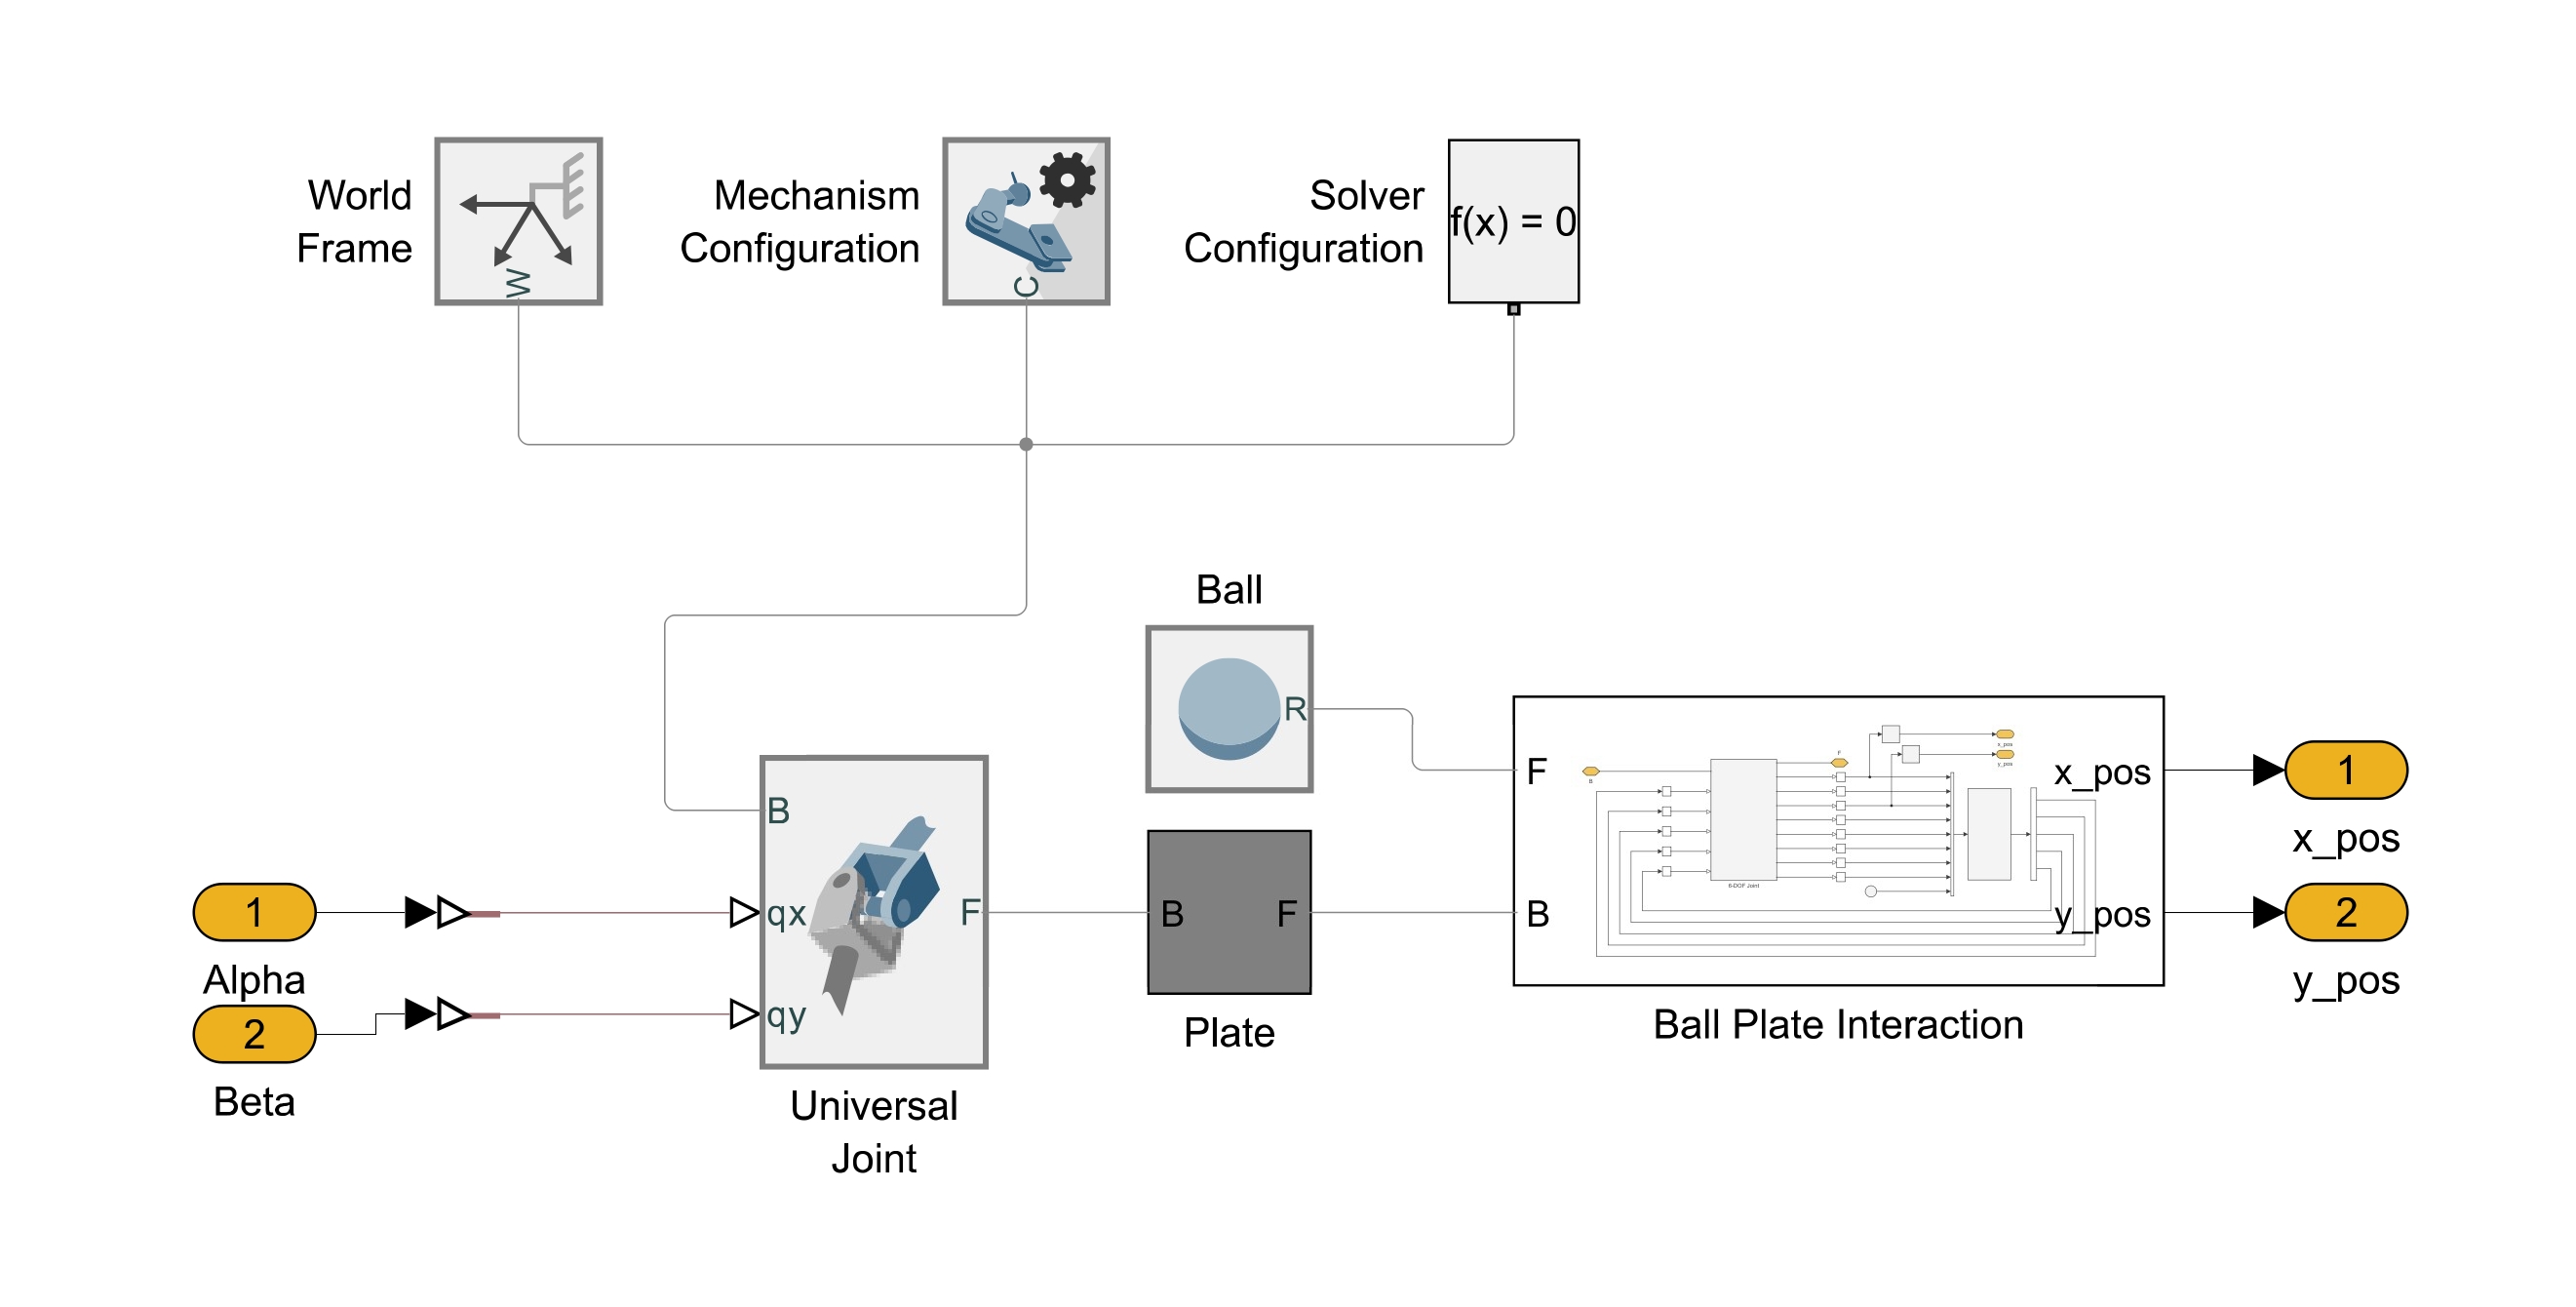
\includegraphics[width=0.95\textheight]{Figures/chapter03/simscape.png}
\caption{Dynamic simulation of the non-linear Ball and Plate System using Simscape}
\label{fig:IMs matrix correlation}
\end{sidewaysfigure}

\begin{sidewaysfigure}
\centering
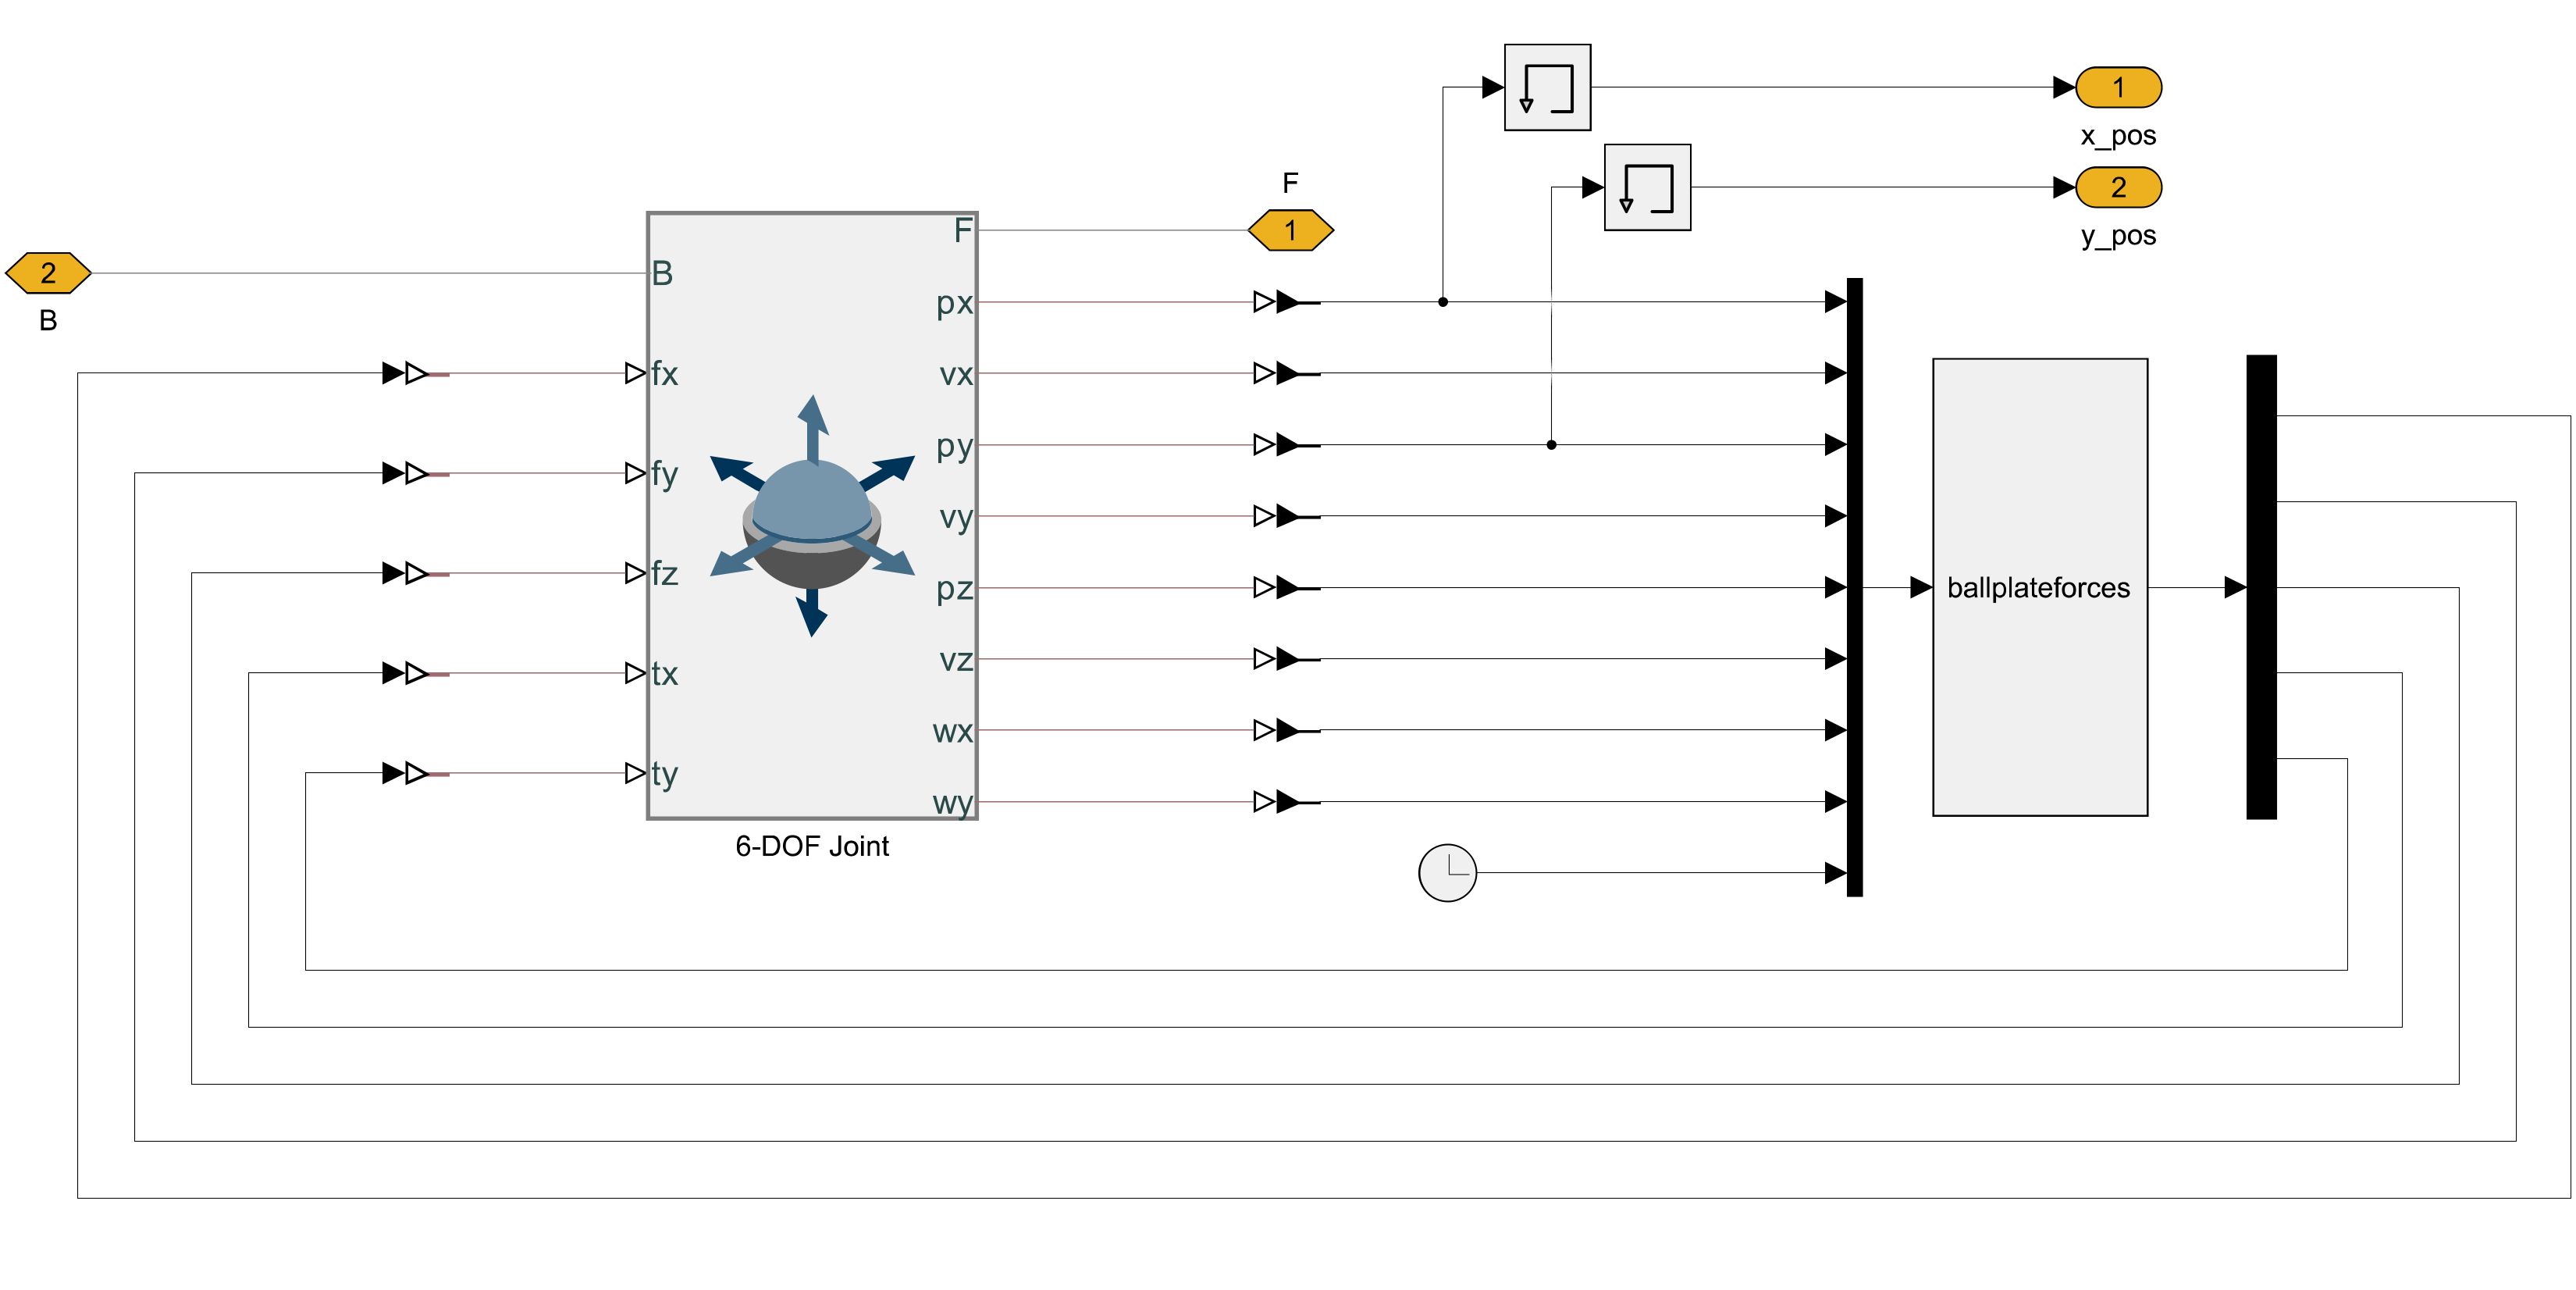
\includegraphics[width=0.95\textheight]{Figures/chapter03/BPinteration.png}
\caption{BPS interaction subsystem}
\label{fig:IMs matrix correlation}
\end{sidewaysfigure}

\begin{sidewaysfigure}
\centering
\includegraphics[width=0.95\textheight]{Figures/chapter04/practicalPID.png}
\caption{PID Simulink Model Illustrating Practical Adjustments: saturation, calibration, white noises, communication delays}
\label{fig:IMs matrix correlation}
\end{sidewaysfigure}

\begin{sidewaysfigure}
\centering
\includegraphics[width=0.95\textheight]{Figures/chapter04/simulink_real_system_pid_model.png}
\caption{Simulink Model used for Controlling the real system}
\label{fig:IMs matrix correlation}
\end{sidewaysfigure}

\begin{sidewaysfigure}
\centering
\includegraphics[width=0.85\textheight]{Figures/chapter04/simulink_real_system_pid_model_subsys.png}
\caption{Simulink Block used for receiving the feedback data}
\label{fig:IMs matrix correlation}
\end{sidewaysfigure}

\chapter{Method of mapping the angles}

In this section, the angular mapping method is utilized to establish the relationship between the input angles and the corresponding output angles of the servomotors. The measurements were obtained using a smartphone, and the linear gains for the mapping were determined as \(k_x = 0.0445\) and \(_y = 0.0377\) by the following matlab code:
\begin{lstlisting}[language=Matlab , caption= matlab code for polynomial fits ]
input = [0,5,10,15,20,25,30,
35,40,45,50,55,60,65,70,75,
80,85,90,95,100,105,110,115,
120,125,130,135,140,145,150,
155,160,165,170,175,180];
output = [-7.9,-7.8,-7.6,-7.2,
-6.9,-6.4,-6,-5.1,-4.6,-3.8,-3,-2.1,-1.4,-0.5, 0.1,0.1,0.5,0.8,1.3,2,2.8,3.6,4.4,5,5.7,6.4,
7,7.6,8.1,9,9.6,9.8,9.9,10.1,10.3,10.4,10.5];
degree = 1;
% polyfit(input,output,degree);
gx = output/input
inputy = [0,5,10,15,20,25,30,35,40,45,
50,55,60,65,70,75,80,85,90,95,100,
105,110,115,120,125,130,135,140,145,150];
outputy=  [7.3,7,6.8,6.6,6.2,5.8,5.3,
4.6,4,3.4,2.7,2.1,1.5,0.7,0.2,0,
-0.9,-1.7,-2.3,-2.9,-3.8,-4.6,-5.3,
-5.8,-6.5,-7,-7.7,-8,-8.6,-9,-9.1];
gy = outputy/inputy
\end{lstlisting}

{\large \textbf{Mapping Values}}

The following table presents the measured input and output angles along with the calculated gains.
\newcolumntype{P}[1]{>{\centering\arraybackslash}p{#1}}
\begin{table}[h]
    \centering
    \begin{tabular}{|P{0.25\linewidth}| P{0.25\linewidth} | P{0.25\linewidth}|}
        \hline
        \textbf{Servomotor Angle (degrees)} & \textbf{Inclination Angle X (degrees)} & \textbf{Inclination  Angle Y (degrees)} \\
        \hline
        0    & -7.9 & 7.3   \\
        5    & -7.8 & 7.0   \\
        10   & -7.6 & 6.8  \\
        15   & -7.2 & 6.6  \\
        20   & -6.9 & 6.2  \\
        25   & -6.4 & 5.8  \\
        30   & -6.0 & 5.3  \\
        35   & -5.1 & 4.6  \\
        40   & -4.6 & 4.0  \\
        45   & -3.8 & 3.4  \\
        50   & -3.0 & 2.7  \\
        55   & -2.1 & 2.1  \\
        60   & -1.4 & 1.5  \\
        65   & -0.5 & 0.7  \\
        70   & -0.1 & 0.2  \\
        75   & 0.1  & 0.0  \\
        80   & 0.5  & -0.9 \\
        85   & 0.8  & -1.7 \\
        90   & 1.3  & -2.3 \\
        95   & 2.0  & -2.9 \\
        100  & 2.8  & -3.8 \\
        105  & 3.6  & -4.6 \\
        110  & 4.4  & -5.3 \\
        115  & 5.0  & -5.8 \\
        120  & 5.7  & -6.5 \\
        125  & 6.4  & -7.0 \\
        130  & 7.0  & -7.7 \\
        135  & 7.6  & -8.0 \\
        140  & 8.1  & -8.6 \\
        145  & 9.0  & -9.0 \\
        150  & 9.6  & -9.1 \\
        155  & 9.8  &  \\
        160  & 9.9  &   \\
        165  & 10.1 &   \\
        170  & 10.3 &   \\
        175  & 10.4 &   \\
        180  & 10.5 &   \\
        \hline
    \end{tabular}
    \caption{Mapping values for input and output angles to calculate the gains.}
    \label{tab:mapping_values}
\end{table}


\end{singlespace}
\bibliographystyle{ieeetr}
\bibliography{myBib}

\end{document}
